\chapter{Corrections to the raw yield}
\label{chap:aCorrection}
\minitoc
\myepigraph{I'll take a drive to Beverly Hills\\
Just before dawn\\
An' knock the little jockeys\\
Off the rich people's lawn\\
An' before they get up\\
I'll be gone, I'll be gone\\
Before they get up\\
I'll be knocking the jockeys off the lawn}{Frank Zappa,
in~\textit{Uncle Remus, Apostrophe (')}}

\externaldocument{pQuarkonia}

\section{Monte Carlo based corrections}
\subsection{Introduction}
As described in Chapter~\ref{chap:pquarkonia}, the \PgU\ production
rate is a rather abundant process at LHC energies, that is detected in CMS by the
means of its dimuon decay, with the help of the muon detectors. Although
the production mechanisms at play are still to settle, we know that
there are three separate resonances, the \PgUa,\PgUb\ and \PgUc\
mesons, each of which decay into two muons in a somewhat standard
QED annihilation process, easily identifiable in the dimuon invariant
mass spectrum produced by $e^{+}e^{-}$, lepton-hadron, hadron-hadron and heavy-ion colliders. The width
of such 'electromagnetic probes' is usually very small with respect to
the current detector resolution, hence a distinct peak can be
measured. Their production rate is estimated by repeating the collision enough
times to record a statistically significant measurement. 

Section~\ref{chap:ayield} established such a rate, that I have called
the~\textit{raw yields}, for our $pp$ and PbPb
samples. Measuring these raw yields was the first step towards estimating two important quantities:
\begin{itemize}
\item[-] The \PgU(nS) production rates in proton-proton collisions, called cross sections, $\sigma\left( pp\rightarrow
\PgU(nS)X\right)$,
\item[-] The corrected invariant yields for \PgU(nS) states in PbPb, $N\left( AA\rightarrow
 \PgU(nS)X\right)$.
\end{itemize}

These two quantities are to be properly normalised in order to obtain
the nuclear modification factor from a direct comparison. This will be
our third step, covered in Chapter~\ref{chap:aupsilon}.

The second step is covered here and consists of translating the raw yields into the
actual number of events produced in the total number of collision
events, whether they were detected or not. This is done by expressing our understanding of what
can alter the \PgU's decay in two muons up to the final step of offline
reconstruction. Indeed, some candidate events are falling out of
the detector sensitive material, and we should account for this, and
some are simply not reconstructed.

Trying to cover the major sources of alteration in the
signal, I have already mentioned the magnetic field, curving slow muons
away from the outer muon chambers, and the \pt\ cuts applied to
the individual muons. These two effects act in the same manner: the total
accessible yield is constrained, reduced. The fraction of dimuon
events that subsisted is defined as the \textit{acceptance}, which
I will detail in Section~\ref{sec:acceptance}. The acceptance is computed in
this case with a simple Monte Carlo simulation, and in principle does
not require the use of detector level quantities, only generator level
quantities, as we shall see.

Another source of alteration in the measurement is the reconstruction
chain. It consists of three main sources, that can be taken as a
common one
for now. This includes the trigger performances, the global muon
reconstruction, and the offline cleaning cuts applied. These effects
are studied from detector based quantities, and for this reason I will
treat them separately from the acceptance (although it is not
unconceivable to see them as only one transfer function). Again,
Monte Carlo simulations are used, this time to estimate the
\textit{efficiency} of triggering, reconstructing, and filtering
offline. The efficiency will be covered in Section~\ref{sec:eff}.

Finally, we will see that both definitions suffer from some
assumptions regarding the simulated sample. The systematic
uncertainties associated to the generated shapes and to the centrality
determination will be treated in Section~\ref{sec:acceff_syst}. In
Section~\ref{sec:data_mc}, the accuracy of the detector simulation
will be tested, and
will open to second order corrections, obtained via a Tag and Probe
method.

\subsection{Acceptance}
\label{sec:acceptance}
The raw \PgU\ yields need to be corrected for the loss of events, caused by the kinematic cuts on the
single muon $\eta$ and $\pt$ that are used in the analysis.
Events are accepted if both muons are in the geometrical acceptance of the
detector, i.e. within $|\eta^{\mu}|<2.4$. The single muon $\pt$ cuts for
\PgUa\ are looser than for \PgUb\ and \PgUc, as was presented in Section~\ref{sec:sigext_fits}.

The acceptance is calculated as:



\begin{equation}
  \alpha(\pt,y) =
  \frac{N^{\mu^{+}\mu^{-}}_{\textrm{detectable},M}(\pt,\y)}{N^{\mu^{+}\mu^{-}}_{\textrm{GEN}\,\in\,\vert\y\vert\,<\,
      2.4}(\pt,\y)},
  \label{eq:acc}
\end{equation}

where the numerator $N^{\mu^{+}\mu^{-}}_{\textrm{detectable},M}$ is
the number of generated events passing the
%$\left(\pt^{\mu^{+}},\pt^{\mu^{-}};\eta^{\mu^{+}},\eta^{\mu^{-}}\right)$
kinematical cuts, and $N^{\mu^{+}\mu^{-}}_{\textrm{GEN}\,\in\,\vert\y\vert\,<\, 2.4}(\pt,\y)$
is the number of events generated, in the (\pt, $y$) analysis bin under consideration, within the coverage of the CMS muon stations.
\\
The acceptance then depends on the single muon $\pt^{\mu}$ cuts applied to the analysis
selection, which are recalled in Table~\ref{tab:kincuts}.
\\
\begin{table}[h]
\begin{center}
  \begin{tabular}{p{2.3cm}p{2.5cm}p{3.2cm}p{3.2cm}}
    \hline
    \PgUa & ``loose cut'' & p$_{T}^{\mu_1} > 3.5$~GeV/$c$ & p$_{T}^{\mu_2} > 4$~GeV/$c$ \\ 
    \PgUb, \PgUc & ``tight cut'' & p$_{T}^{\mu_1} > 4$~GeV/$c$ & p$_{T}^{\mu_2} > 4$~GeV/$c$ \\
    \hline        
  \end{tabular}
  \caption{Denominations and definitions of the cuts used in the \PgUa\ analysis and in
    the \PgUb\ and \PgUc\ analysis.}
  \label{tab:kincuts}
\end{center}
\end{table}


Since a non-zero quarkonium polarisation would impact the angular
dimuon distributions, previous analyses~\cite{atlasUpsilon7tev,cmsUpsi1} used to study the effect of
various polarisation configurations on the acceptance. Hence,
Equation~\ref{eq:acc} should also exhibit a dependence on a
polarisation anisotropy parameter $\lambda_{\vartheta}$, itself depending on a choice of
polarisation frame.  We have seen in Chapter~\ref{chap:pquarkonia} the effect of
various polarisation scenarii, in Figure~\ref{fig:atlasNNLO} (the
light blue band corresponding to various \textit{spin alignment
  configurations}, as quoted
in~\cite{atlasUpsilon7tev}).~\cite{cmsUpsi1} reports that in the
phase space of this analysis (low \PgU\ \pt, and $\vert\eta\vert <
2.4$), 
anisotropies of $\pm 0.25, \pm 0.5$ and
$\pm 1$ would vary the obtained ($pp$) cross sections by about  $\pm
5\%, \pm 10\%, \pm 20\%$, respectively.



However, it has been recently measured in~\cite{CMSupsipol} that the
\PgU\ polarisation in the phase space covered by CMS is small, up to a
higher \pt\ range than what is covered in this analysis. For this
reason, the acceptance is not accounting for other possibilities than
the non-observed polarisations of \PgUa, \PgUb, \PgUc.


If the polarisation were to change in heavy ion collisions, this would
be an effect of the underlying physics in the medium in which the
quarkonia are produced. Different polarisations between $pp$ and PbPb
would mean different angular distributions for single muons in the laboratory
frame. Having the same single muon cuts in $pp$ and PbPb, a
polarisation modification should hence reflect itself in the nuclear
modification factor \RAA, that we shall present in
Chapter~\ref{chap:aupsilon}. 



The acceptance being a quantity computed with generator-based number
of events, we
assume it is independent on the collision system\footnote{Unless the
 different collision systems are asymmetric, as in the case of p-A collisions. In such cases, the acceptance needs to be recomputed
 separately, the centre of mass of the collision not being at rest in
 the laboratory frame.}. Hence, there is only one acceptance
computation for each state. \PgU\ mesons are generated using official CMS
configuration files for PYTHIA~\cite{Sjostrand:2006za} particle
generation. After making sure there is no
kinematic filter in the generation, I have generated 1 million events for each state.%  The specifics of the generation
% are gathered in Table~\ref{tab:GenSamples}.
% \begin{table}[h]
% \begin{centering}
% \begin{tabular}{|c|c|}                                      
% \hline
% Generation software & Pythia 6.4\\
% $\sqrt{s}$ & 2.76 TeV \\
% Decay modes & $\mu^{+}\mu^{-}$ only\\
% %\multiline{2}{l}{number of events}
% \hline
% \end{tabular}
% \caption{Generation parameters used for our simulation samples}  
% \label{tab:GenSamples}
% \end{centering}
% \end{table}



The acceptance is computed separately for each \PgU\ state, and its value
is by definition a number between 0 and 1, dependent on the
considered portion of the ($\pt(\PgU)$, $\vert\y(\PgU)\vert$) plane. In
Figure~\ref{fig:fineBins}, a smooth distribution of the generated
\PgUa\ events is shown before and after applying the kinematic cuts of
the analysis (left and right, respectively). I have removed the
binning of the analysis in both panels, to get a better sense of how
the events are distributed along \pt\ and rapidity. The z-axis is
identical, to illustrate the loss in
statistics after applying the acceptance cut.
\begin{figure}[h]
\begin{centering}  
  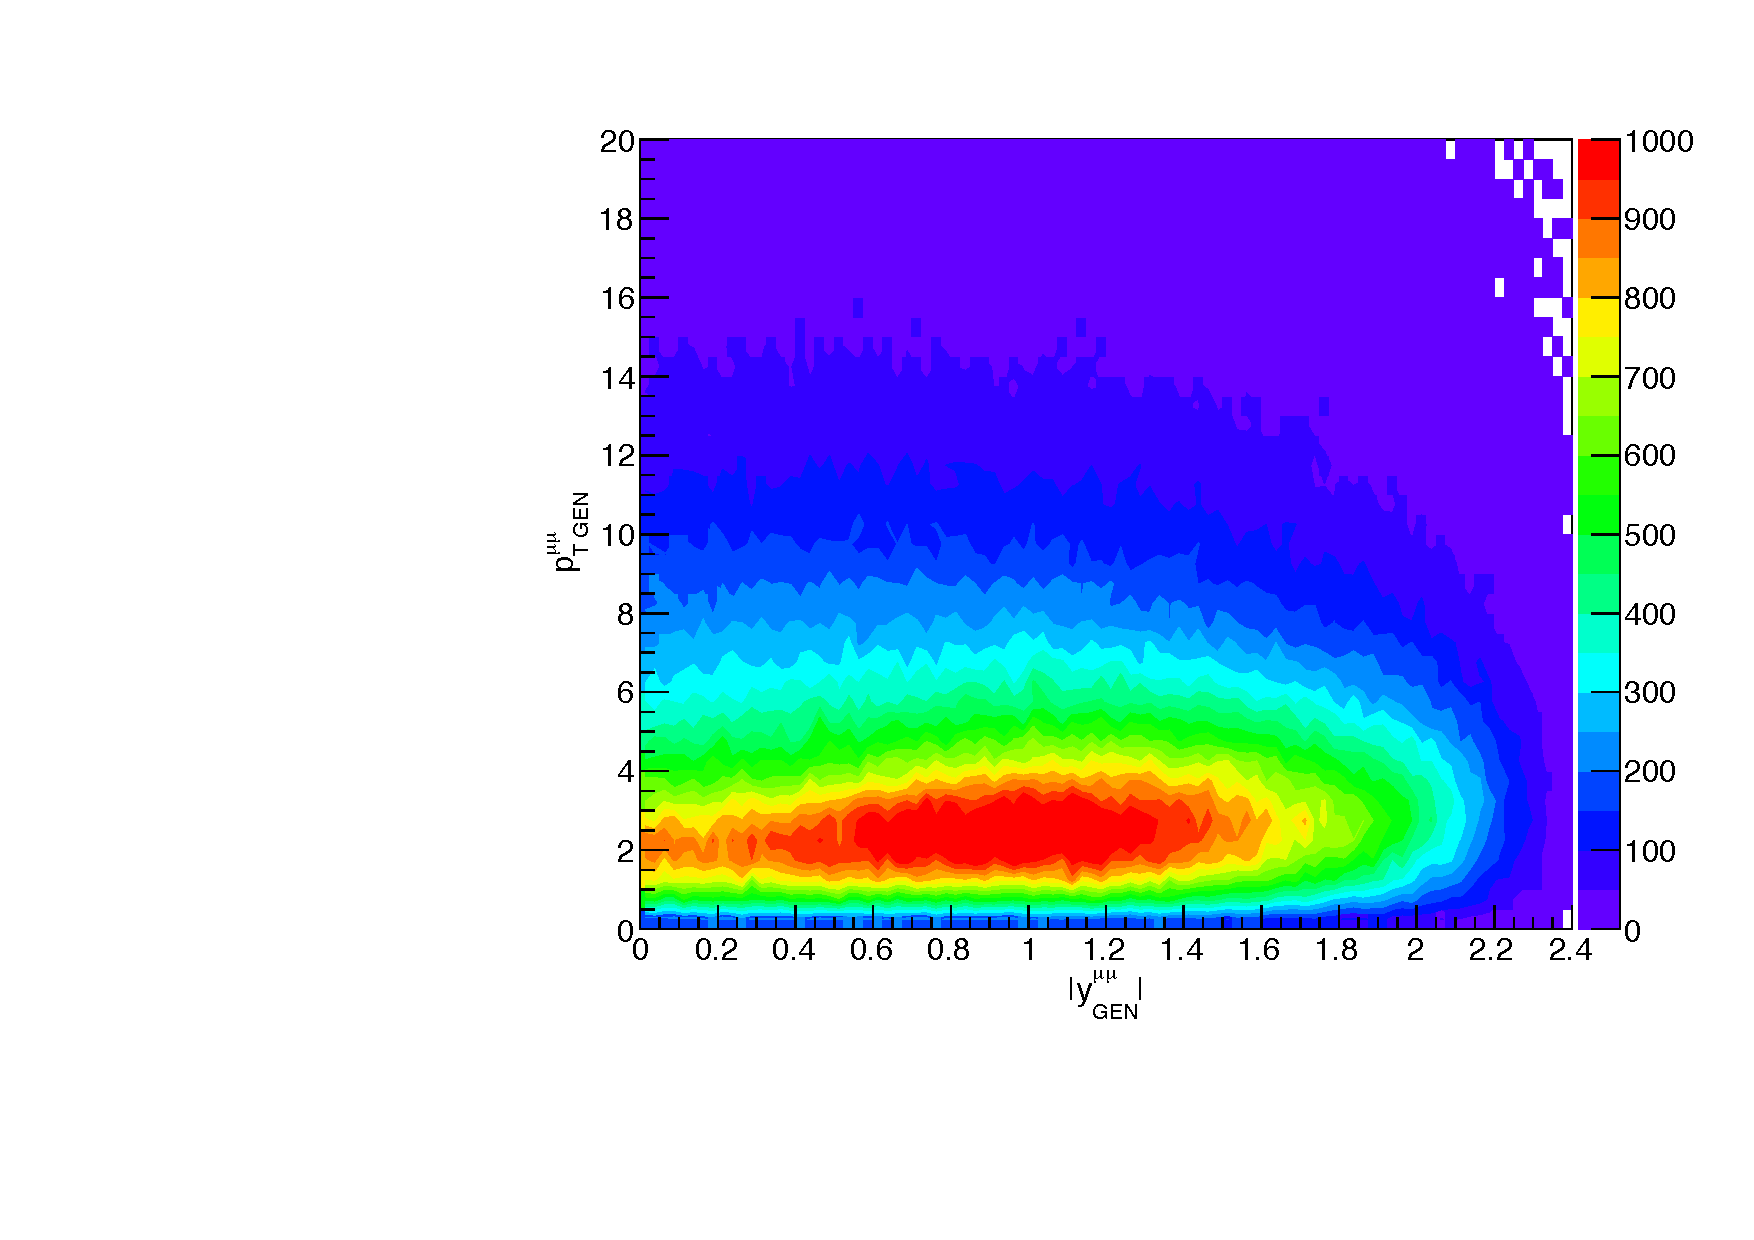
\includegraphics[width=0.49\textwidth]{Chapters/aCorrection/simple_yPt.pdf}
  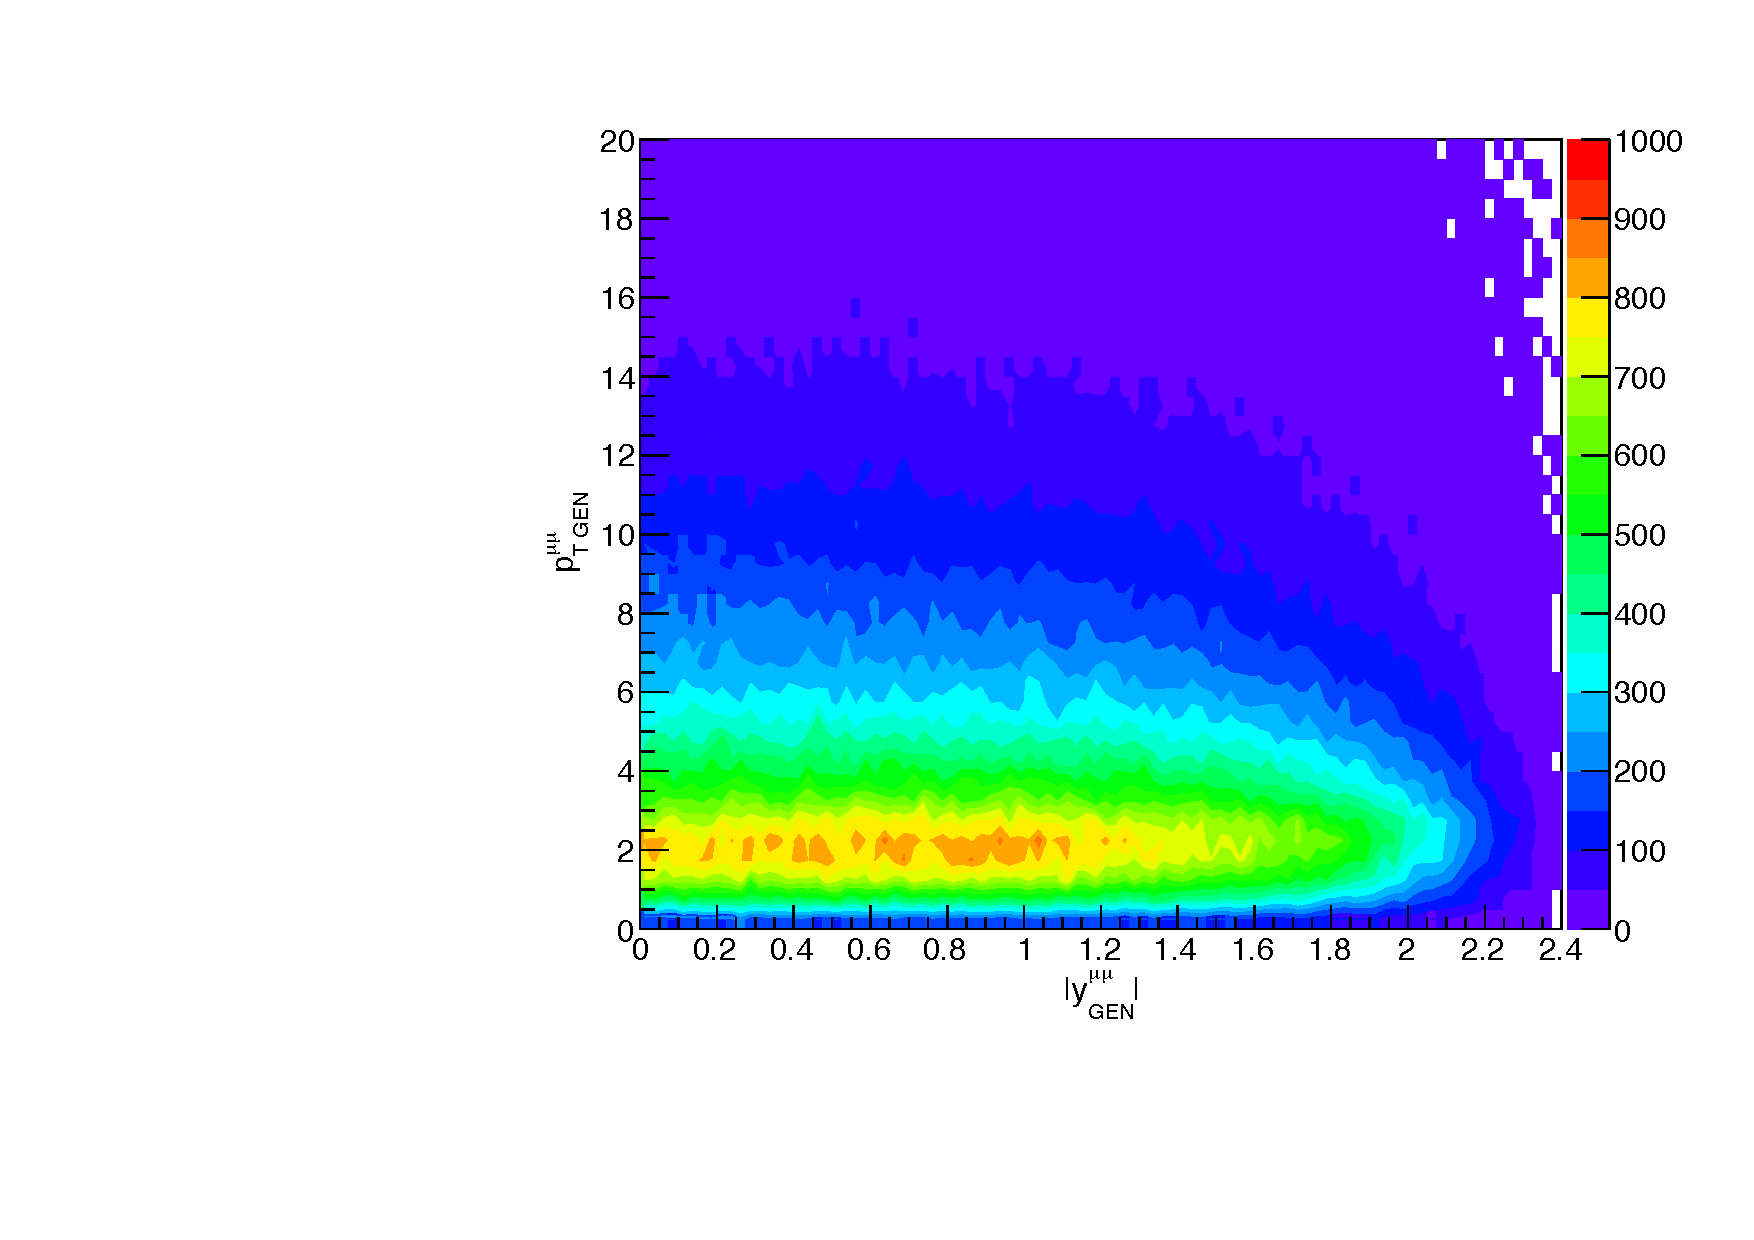
\includegraphics[width=0.49\textwidth]{Chapters/aCorrection/Acc_yPt.pdf}
  \caption{Phase space maps of the \PgUa\ generation sample: left, no
    cut applied; right, loose acceptance cut applied. A smooth
    contour drawing option is used.}
  \label{fig:fineBins} 
\end{centering}  
\end{figure}


The denominator of acceptance is represented by the
left-hand-side plot, and the numerator appears to the right.
%  of
% Figure~\ref{fig:fineBins}, while 
The (\pt,$\vert y\vert$) binning presented in
Section~\ref{sec:sigext_yield} is used to extract the acceptance
corrections for the \pt- and \y-differential analyses of each \PgU\
state. The binned results for \acc(\pt,y) are presented for \PgUa\ in Table~\ref{tab:acceptance1} with
their statistical uncertainties (small since the MC
samples used are very large).



\begin{table}
\begin{center}
\begin{tabular}{|c|c||c|c|}
\hline
\pt [\GeVc]& \acc[1S](\pt)      & $\vert\y\vert$     &      \acc[1S](\y) \\
% \hline
% 0.000-5.000     &0.357 $\pm$ 0.001   &  \\
% 5.000-12.000    & 0.309 $\pm$ 0.001  &  \\
% 12.000-20.000   & 0.513 $\pm$ 0.005  &  \\
\hline                                       
0-2.5             &  0.456 $\pm$ 0.002  & 0-0.4   & 0.393 $\pm$ 0.002  \\
2.5-5             &  0.298 $\pm$ 0.001  & 0.4-0.8 & 0.392 $\pm$ 0.002  \\
5-8               &  0.277 $\pm$ 0.001  & 0.8-1.2 & 0.393 $\pm$ 0.002  \\
8-12              &  0.374 $\pm$ 0.002  & 1.2-1.6 & 0.389 $\pm$ 0.002  \\
12-20             &  0.513 $\pm$ 0.005  & 1.6-2   & 0.338 $\pm$ 0.002\\
\cline{1-2}
\textbf{0-100}             &  \textbf{0.353 $\pm$ 0.001}  & 2-2.4   & 0.145 $\pm$ 0.001  \\
\hline                          
\end{tabular}
\caption{Acceptance correction factors as a function of \pt\ and \y\ for
  $\Upsilon$(1S). The left hand side contains the results for a \pt\
  dependent binning. The right hand side contains the results for a
  rapidity-dependent binning. On the left hand side, the last entry at
the bottom (boldfaced) corresponds to the integrated result.}
\label{tab:acceptance1}
\end{center}
\end{table}


The excited states, as we have seen in Table~\ref{tab:kincuts},
are analysed with a tighter cut. Furthermore, the
strong suppression seen in PbPb collisions for the excited states did
not allow for such a fine binning as used for the $pp$
yields. Coincidentally, Table~\ref{tab:acceptance2} has the
acceptance for \PgUb\ in two different sets of bins: the fine ones
are used in the \PgUb\ pp cross section, while coarser ones are
used for the PbPb invariant yields. 

\begin{table}
  \begin{center}
    \begin{tabular}{|c|c||c|c|}
      \hline
      \pt [\GeVc]& \acc[2S](\pt)      & $\vert\y\vert$   &      \acc[2S](\y) \\
      \hline                                       
      0-2.5             & 0.375 $\pm$ 0.002  & 0-0.4   &  0.310 $\pm$ 0.002 \\
      2.5-5             & 0.217 $\pm$ 0.001  & 0.4-0.8 &  0.310 $\pm$ 0.002 \\
      5-8               & 0.218 $\pm$ 0.002  & 0.8-1.2 &  0.307 $\pm$ 0.002 \\
      8-12              & 0.309 $\pm$ 0.003  & 1.2-1.6 &  0.308 $\pm$ 0.002 \\
      12-20             & 0.467 $\pm$ 0.007  & 1.6-2   &  0.271 $\pm$
      0.002 \\
\cline{1-2}
      \textbf{0-100}             &  \textbf{0.279 $\pm$ 0.001} & 2-2.4   &  0.117 $\pm$ 0.001 \\
      \hline
      0-5              & 0.357 $\pm$ 0.001  & 0-1.2   &  0.309 $\pm$ 0.001 \\
      5-12             & 0.309 $\pm$ 0.001  & 1.2-2.4 &  0.241 $\pm$ 0.001 \\
      12-20            & 0.513 $\pm$ 0.005  &      -  &   -         \\
      \hline                           
    \end{tabular}
    \caption{Acceptance correction factors as a function of \pt\ and \y\ for
      $\Upsilon$(2S). The left hand side contains the results for a \pt\
      dependent binning. The right hand side contains the results for a
      rapidity-dependent binning. Bold font is used for the integrated
      result. The bottom panel has a coarser binning, corresponding to the
      PbPb analysis.}
    \label{tab:acceptance2}
  \end{center}
\end{table}

% Since the \PgUc\ state is not observed in PbPb collisions, the
% acceptance values are only needed in the pp cross section
% computation. Acceptance corrections cancel in the ratio
%  used to compute the
% confidence interval on \PgUc\ suppression.

As we have seen in Chapter~\ref{chap:ayield}, the \PgUc\ yield is
unobserved in PbPb. As a result, a confidence interval on the
suppression of \PgUc\ will be presented later in
Chapter~\ref{chap:aupsilon}, in which acceptance corrections would
cancel in the ratio \NFitThreeS|$_{\textrm{PbPb}}$/\NFitThreeS|$_{pp}$. For this reason, the \PgUc\ acceptance presented in
Table~\ref{tab:acceptance3} only applies to the $pp$ \PgUc\ cross
section.

\begin{table} [h]
  \begin{center}
    \begin{tabular}{|c|c||c|c|}
      \hline
      \pt [\GeVc]& \acc[3S](\pt)      & $\vert\y\vert$     &      \acc[3S](\y) \\
      \hline                                       
      0-2.5             & 0.455 $\pm$ 0.001  & 0-0.4   & 0.367 $\pm$ 0.001  \\
      2.5-5             & 0.273 $\pm$ 0.001  & 0.4-0.8 & 0.366 $\pm$ 0.001  \\
      5-8               & 0.249 $\pm$ 0.001  & 0.8-1.2 & 0.366 $\pm$ 0.001  \\
      8-12              & 0.330 $\pm$ 0.001  & 1.2-1.6 & 0.361 $\pm$ 0.001  \\
      12-20             & 0.471 $\pm$ 0.002  & 1.6-2   & 0.312 $\pm$
      0.001  \\
\cline{1-2}
      \textbf{0-100}             &  \textbf{0.329 $\pm$ 0.000} & 2-2.4   & 0.136 $\pm$ 0.001  \\
      \hline                           
    \end{tabular}
    \caption{Acceptance correction factors as a function of \pt\ and \y\ for
      $\Upsilon$(3S). The left hand side contains the results for a \pt\
      dependent binning. The right hand side contains the results for a
      rapidity-dependent binning. Bold font is used for the integrated
      result. These factors are only used in the $pp$ cross section calculation.}
    \label{tab:acceptance3}
  \end{center}
\end{table}



\vspace{1.2cm}
Looking at the values obtained for \acc\ in all three states, we see
that acceptances vary over the \pt\ and rapidity range studied. For
example, let me compare the acceptance of \PgUa\ as a function of
its transverse momentum, to the integrated value, $\acc(\PgUa) = 0.353
\pm 0.001$. 

While it is approximately $30 \%$ higher in the lowest
\pt\ bin ($\acc(\pt \in [0.,2.5] \GeVc) = 0.456 \pm 0.002$), \acc(\PgUa)
decreases when $5 < \pt < 8~\GeVc$, to rise again at higher
momenta. This can be understood when judging the kinematics of the
$\PgU \to \mu\mu$ decay:

\begin{itemize}
\item[-] When the resonance is produced almost at rest, the rest
  energy is of the order of the quarkonium's rest mass, $E \sim
  m_{\PgU}$. In this case, it will often occur that both muons will
  carry an energy of about
  $E_{\mu} \sim m_{\PgU}/2 \approx 5~\unitMass$, which is enough to
  reach the muon stations (i.e. `fall in the acceptance of the
  detector');
\item[-] When the resonance rest frame is boosted with respect to the
  laboratory frame, the decay will appear asymmetric to the observer, with one muon
  carrying a larger fraction of the available decay momemtun than the
  other. Then, if the \PgU\ is produced at a moderate \pt, say,
  between 3 and 8
  \GeVc, it is likely that one of the muons will have a momentum
  $p^{\mu}_{LAB}$ such that $\pt^{\mu} < \pt(\rm{cut})$. In this case
  the event does not pass the kinematic cut, and is lost;
\item[-] Finally reaching higher quarkonium momenta, both muons carry
  a large momentum and the acceptance increases again.
\end{itemize}

\fbox{
  \parbox{0.9\textwidth}
  {\textsf{In this paragraph I have presented the acceptance, a
      computation of the number of \PgU\ events passing the
      kinematical selection. This answered the question: ``after producing $X$ events of
      interest, what is \acc\ such that $\acc X$ is the fraction of
      detectable events?''. As we shall see in Section~\ref{sec:acceff_syst}, the number $X$ is not
      taken arbitrarily, as the kinematics of the
      production assumed by PYTHIA are varied to extract a systematic
      uncertainty on \acc.}
  }
}

\vfill~\\

\subsection{Efficiency}
\label{sec:eff}
The efficiency has been introduced above, saying that this correction
accounts for all the other selection steps, namely: the trigger, the
actual reconstruction chain that makes global dimuon pairs, and the
offline quality and muon identification cuts. I have asserted that these sources can be treated in only one black box,
with a single correction factor \eff. Let me anticipate and say that
although it is true at first order, a study has been done to assess the
second order of this correction. This study has the advantage of being
data-driven, so it also allows to gauge the level of understanding of
our simulation of the detector. This so called \textit{Tag and Probe}
study is covered in Section~\ref{sec:tnp}.




The dimuon efficiency \eff\ is defined as
\begin{eqnarray}
\varepsilon(\pt,y,\textrm{cent.}) & = &
\frac{N^{\mu^{+}\mu^{-}}_{\textrm{Reco.}, M \in [R]}(\pt,y,\textrm{cent.})}{N^{\mu^{+}\mu^{-}}_{\textrm{detectable},M}(\pt,\y)}. 
\label{eq:efficiency}
\end{eqnarray}


%{fig:fineBins} 
Comparing with Equation~\ref{eq:acc}, it is important to note that the
denominator of \eff, $N^{\mu^{+}\mu^{-}}_{\textrm{detectable},M}$, is
the numerator of \acc, as defined above. This is the number of events
that passed the kinematical cuts, i.e. falling in the acceptance of
the detector.

The numerator of \eff,
$N^{\mu^{+}\mu^{-}}_{\textrm{Reco.}, M \in [R]}$, is the number of
dimuon events reconstructed in the (\pt, \y, cent.)-bin under
consideration. These events have passed all selection criteria of the
analysis, namely:
\begin{itemize}
\item[-]Two muons have fired the emulated version of the L1 trigger
 \verb?L1DoubleMuOpen?, further filtered at HLT for \verb?_HighQ?,
 which requests a confirmed signal from two combinations of RPC, CSC
 and DT subdetectors, as defined in Section~\ref{sec:evtsel};
\item[-]The muons have deposited enough hits in the muon stations to form
  \textit{standalone muons},
\item[-]These standalones could be matched to tracker tracks forming
  \textit{global muon} refitted objects,
\item[-]Each global muon have passed the series of tracker and global
  quality cuts defined in Section~\ref{sec:muonID},
\item[-]The combination of these global muons has resulted in a dimuon candidate
  falling in the \PgU\ mass region [$R$].
\end{itemize}

% The generated dimuons must have both single muons generated within the
% acceptance cuts discussed above.
% Considering the mass interval [$R$], one can either define it being
% the mass interval around the resonance peak, wide enough (typically to
% or three times the peak width) to two ways have been envisioned:
% either cutting at the 
The dimuons are counted in the mass interval [$R_{1S}$] $\equiv$ [8.0, 10.5] \GeVc for $\Upsilon$(1S),
in [$R_{2S}$] $\equiv$ [8.5, 11] \GeVc  for $\Upsilon$(2S) and in [$R_{3S}$]
$\equiv$ [8.8, 11.3] \GeVc for $\Upsilon$(3S). Although the mass
regions do overlap, there is no cross talk, since each state was
simulated separately.

The numerator $N^{\mu^{+}\mu^{-}}_{\textrm{Reco.}, M \in [R]}$ can also
depend on the centrality of the heavy ion event. The HYDJET events are
generated flat in centrality, and there is one PYTHIA \PgU\ embedded
in every event. I have thus removed the
centrality dependence in the denominator of Equation~\ref{eq:acc},
which is a generation level quantity, as
well as in Equation~\ref{eq:efficiency}. However, the heavy ion multiplicity
environment may have an impact on the reconstruction or triggering
performances, inducing a multiplicity dependence. As a result, the
$pp$ and PbPb efficiencies are not equal, and are computed separately for each collision
setup.


The \pt- and \y-dependent results for \PgUa\ are reported in
Table~\ref{tab:Y1Seff}. The heavy ion efficiencies
\eff$_{\rm PbPb}$ are slightly outperformed by the pp reconstruction
efficiency \eff$_{pp}$, especially at low \pt, where there is an
approximately 10 \% difference.


\begin{table}
\begin{center}
\begin{tabular}{|c|c|c||c|c|c|}
\hline
\pt [\GeVc]&\eff[1S]$_{pp}$&\eff[1S]$_{\rm PbPb}$&
|\y|    &  \eff[1S]$_{pp}$&\eff[1S]$_{\rm PbPb}$\\
\hline                                                            
0-2.5             &0.659 $\pm$ 0.002   & 0.589 $\pm$ 0.005  & 0-0.4   & 0.709 $\pm$ 0.003   &0.611 $\pm$ 0.005\\
2.5-5             &0.648 $\pm$ 0.002   & 0.588 $\pm$ 0.005  & 0.4-0.8 & 0.711 $\pm$ 0.003   &0.639 $\pm$ 0.006\\
5-8               &0.686 $\pm$ 0.003   & 0.651 $\pm$ 0.006  & 0.8-1.2 & 0.713 $\pm$ 0.003   &0.674 $\pm$ 0.006\\
8-12              &0.716 $\pm$ 0.004   & 0.712 $\pm$ 0.005  & 1.2-1.6 & 0.674 $\pm$ 0.003   &0.656 $\pm$ 0.006\\
12-20             &0.757 $\pm$ 0.005   & 0.753 $\pm$ 0.005  & 1.6-2
& 0.615 $\pm$ 0.003   &0.611 $\pm$ 0.007\\
\cline{1-3}
\textbf{0-100}             &\textbf{0.679 $\pm$ 0.001}&\textbf{0.633 $\pm$ 0.003}& 2-2.4   & 0.500 $\pm$ 0.004   &0.521 $\pm$ 0.010\\
\hline                           
\end{tabular}
\caption{Efficiency correction factors as a function of \pt\ and \y\ for
  $\Upsilon$(1S). From left to right, in order of appearance: \pt
  binning, $pp$ efficiency \vs. \pt, PbPb efficiency \vs. \pt, rapidity binning, $pp$
  efficiency \vs. \y, PbPb efficiency \vs. \y. In bold font appears the
  integrated result for \eff[1S]$_{pp}$ (left) and
  \eff[1S]$_{\rm{PbPb}}$ (right). }
\label{tab:Y1Seff}
\end{center}
\end{table}

% We also need a centrality dependent measurement of the efficiency in
% PbPb, to compute the nuclear modification as a function of the
% collision centrality.
The centrality dependent efficiency
\eff$_{\textrm{PbPb}}$ for \PgUa\ is presented in
Table~\ref{tab:centeff}. There, one can notice that the efficiency does
not vary with the event centrality by more than 8\%, from the most
peripheral to the most central events.


\begin{table}
\begin{center}
\begin{tabular}{|c|c|}
\hline
   Centrality & \eff[1S](Cent.)$_{\rm PbPb}$ \\
\hline
0\%-5\%   & 0.606 $\pm$ 0.007  \\
5\%-10\%  & 0.626 $\pm$ 0.008  \\
10\%-20\% & 0.636 $\pm$ 0.006  \\
20\%-30\% & 0.646 $\pm$ 0.006  \\
30\%-40\% & 0.648 $\pm$ 0.006  \\
40\%-50\% & 0.651 $\pm$ 0.006  \\
50\%-70\% & 0.657 $\pm$ 0.004  \\
70\%-100\%& 0.656 $\pm$ 0.004  \\
\hline
\end{tabular}
\caption{$\Upsilon$(1S) reconstruction efficiency as a function of centrality in
  PbPb. Increasing centrality percentiles correspond to lower
  multiplicities (e.g., the first line reads as the efficiency for the
  5\% most central events).}
\label{tab:centeff}
\end{center}
\end{table}


Table~\ref{tab:2Sppeff} sums up the efficiencies \eff[2S]$_{pp}$ used
in \pt- and rapidity dependent $pp$ cross sections. As mentioned
earlier, the PbPb analysis of \PgUb\ makes use of a different binning; For this reason,
Table~\ref{tab:2SppPbPbeff} contains PbPb efficiencies \vs. \pt\ and
\y\ along with the corresponding $pp$ efficiencies recomputed to reflect the proper binning.


\begin{table}
\begin{center}
\begin{tabular}{|c|c||c|c|}
\hline
\pt [\GeVc]&\eff[2S](\pt)$_{pp}$&|\y|    &  \eff[2S](\y)$_{pp}$\\
\hline                                                            
0-2.5             &  0.721 $\pm$ 0.002 & 0-0.4   & 0.791 $\pm$ 0.004 \\
2.5-5             &  0.729 $\pm$ 0.003 & 0.4-0.8 & 0.795 $\pm$ 0.004 \\
5-8               &  0.744 $\pm$ 0.004 & 0.8-1.2 & 0.781 $\pm$ 0.004 \\
8-12              &  0.758 $\pm$ 0.005 & 1.2-1.6 & 0.726 $\pm$ 0.004 \\
12-20             &  0.784 $\pm$ 0.007 & 1.6-2   & 0.643 $\pm$ 0.004
\\
\cline{1-2}
\textbf{0-100}             & \textbf{0.743 $\pm$ 0.002}  & 2-2.4   & 0.519 $\pm$ 0.005 \\
\hline                   
\end{tabular}
\caption{Efficiency correction factors of \PgUb\ in $pp$, as a function of \pt\ and \y. From left to right, in order of appearance: \pt
  binning, efficiency \vs. \pt, rapidity binning, efficiency
  \vs. \y. The integrated result \eff[2S]$_{pp}$ is in bold.}
\label{tab:2Sppeff}
\end{center}
\end{table}

In Table~\ref{tab:2SppPbPbeff}, it can again be seen that the pp
efficiencies are slightly higher than the PbPb ones. The
centrality dependent efficiencies of the \PgUb\ PbPb analysis are
shown in Table~\ref{tab:2Scenteff}.


\begin{table}[h]
\begin{center}
\begin{tabular}{|c|c|c||c|c|c|}
\hline
\pt [\GeVc]&\eff[2S](\pt)$_{pp}$&\eff[2S](\pt)$_{PbPb}$&
|\y|    &  \eff[2S](\y)$_{pp}$&\eff[2S](\y)$_{PbPb}$\\
\hline                                                            
0-5             & 0.726 $\pm$ 0.002  & 0.692 $\pm$ 0.005  & 0-1.2   &0.789 $\pm$ 0.002 & 0.747 $\pm$ 0.004 \\
5-12            & 0.750 $\pm$ 0.003  & 0.741 $\pm$ 0.005  & 1.2-2.4
&0.666 $\pm$ 0.002 & 0.681 $\pm$ 0.005 \\
\cline{4-6}
12-20           & 0.784 $\pm$ 0.007  & 0.789 $\pm$ 0.004  & \textbf{0-2.4}  & \textbf{0.743 $\pm$ 0.002} &  \textbf{0.722 $\pm$ 0.003}\\
\hline               
\end{tabular}
\caption{Efficiency correction factors of \PgUb\ in $pp$ and PbPb, as a function of \pt\ and \y\ for, in bins of the PbPb analysis.  
 From left to right, in order of appearance: \pt
  binning, $pp$ efficiency \vs. \pt, PbPb efficiency \vs. \pt, rapidity binning, $pp$
  efficiency \vs. \y, PbPb efficiency \vs. \y. In bold font appears
  the integrated results for \eff[2S]$_{pp}$ (left) and
  \eff[2S]$_{\rm{PbPb}}$ (right).}
\label{tab:2SppPbPbeff}
% \end{center}
% \end{table}
\vspace{0.3cm}
% \begin{table}[h]
% \begin{center}
\begin{tabular}{|c|c|}
\hline
   Centrality & \eff[2S](Cent.)$_{\rm PbPb}$ \\
\hline
0\%-10\%  & 0.698 $\pm$ 0.008 \\
10\%-30\% & 0.724 $\pm$ 0.005 \\
30\%-50\% & 0.734 $\pm$ 0.005 \\
50\%-100\%& 0.742 $\pm$ 0.004 \\
\hline
\end{tabular}
\caption{Reconstruction efficiency as a function of centrality for
  $\Upsilon$(2S) in PbPb collisions.}
\label{tab:2Scenteff}
\end{center}
\end{table}


Table~\ref{tab:3Sppeff} sums up the efficiencies \eff[3S]$_{pp}$ used
in \pt- and rapidity dependent $pp$ cross sections. Given the fact
that \PgUc\ was not observed in PbPb, we did not decide to generate a
large sample to estimate the \PgUc\ reconstruction
efficiency.

However, an estimation of what would be the efficiency for \PgUc\ in PbPb can be computed,
assuming that the ratio of $pp$ and PbPb efficiencies stays the same
for \PgUc\ as it is for \PgUb:
\begin{equation}
\frac{\eff[3S]_{\rm{PbPb}}}{\eff[3S]_{pp}} \approx
\frac{\eff[2S]_{\rm{PbPb}}}{\eff[2S]_{pp}} = 0.972
\label{eq:eff3S}
\end{equation}
Using this scaling factor and the integrated efficiency in
$pp$,  \eff[3S]$_{pp}$ = 0.752 $\pm$ 0.001, we get an efficiency \eff[3S]$_{\rm{PbPb}}$ = 0.731, that will
be used in the computation of the upper limit on \PgUc\ suppression in PbPb.

\begin{table}
\begin{center}
\begin{tabular}{|c|c||c|c|}
\hline
\pt [\GeVc]&\eff[3S](\pt)$_{pp}$&
|\y|    &  \eff[3S](\y)$_{pp}$\\
\hline                                                            
0-2.5            &  0.731 $\pm$ 0.003 & 0-0.4    & 0.804 $\pm$ 0.003\\
2.5-5            &  0.732 $\pm$ 0.002 & 0.4-0.8  & 0.804 $\pm$ 0.003\\
5-8              &  0.751 $\pm$ 0.003 & 0.8-1.2  & 0.787 $\pm$ 0.003\\
8-12             &  0.769 $\pm$ 0.003 & 1.2-1.6  & 0.734 $\pm$ 0.003\\
12-20            &  0.795 $\pm$ 0.004 & 1.6-2    & 0.649 $\pm$ 0.003\\
\textbf{0-100}           & \textbf{ 0.752 $\pm$ 0.001} & 2-2.4    & 0.522 $\pm$ 0.005\\
\hline                   
\end{tabular}
\caption{Efficiency correction factors of \PgUc\ in $pp$, as a function of \pt\ and \y. From left to right, in order of appearance: \pt
  binning, efficiency \vs. \pt, rapidity binning, efficiency \vs. \y. In bold font appears
  the integrated results for \eff[3S]$_{pp}$.}
\label{tab:3Sppeff}
\end{center}
\end{table}


% This paragraph and the previous one were meant to introduce the
% corrections to apply to get the physical yield of \PgU\ passing
% through the detector.
\vspace{0.3cm}
\fbox{
  \parbox{0.9\textwidth}
  {\textsf{The question answered at the end of the
      acceptance paragraph can be directly extended to acceptance times efficiency: ``after producing $X$ events of
      interest, out of which \acc$X$ were detectable, what is \eff\ such that \acc\eff$X$ is the fraction of
      detected events?''. The importance of the assumed spectrum for $X$ has
      been mentioned already, and impacts both \acc\ and \eff. The next
      paragraph will test the various assumptions on generated shapes and thus
      will provide an estimate of the systematic uncertainty coming from
      these assumptions.}
  }
}



\subsection{Systematic uncertainties}
\label{sec:acceff_syst}
\subsubsection*{From the generated \texorpdfstring{\PgU}{y} spectrum}
% In Section~\ref{sec:acceptance}, I have mentioned that the generated
% sample for \PgU\ was from a Pythia 6.4 simulation, including no
% underlying event, and using a HYDJET embedding only for the purpose of
% studying the effect of the heavy-ion
% multiplicity on the overall dimuon reconstruction, hence not impacting
% the results at the level of the acceptance.

 To validate the strategy used for acceptance and efficiency,
I have compared the generated spectra of \PgU\ states (in other words,
the physical spectrum that PYTHIA assumes as 'true') to the final pp cross
section results, obtained after signal extraction and applying all
corrections, including the Tag and Probe presented in the next Section. The differences seen in \PgUa,\PgUb\ and \PgUc\ \pt\
distributions between PYTHIA and pp data can be seen in the following
Figure~\ref{fig:pythia_data}, alongside with their respective ratios
(Data/PYTHIA). These ratios seem to increase linearly with
\pt, so this trend was fitted to a straight line to obtain a
re-weighting of the generated spectra. The same procedure was applied
to rapidity-differential cross sections.% The final cross section used here is in fact presented in
% Section~\ref{sec:results_pp}. The comparison between 'MC truth' and
% 'physics' is reported.

\begin{figure}
\begin{centering}  
  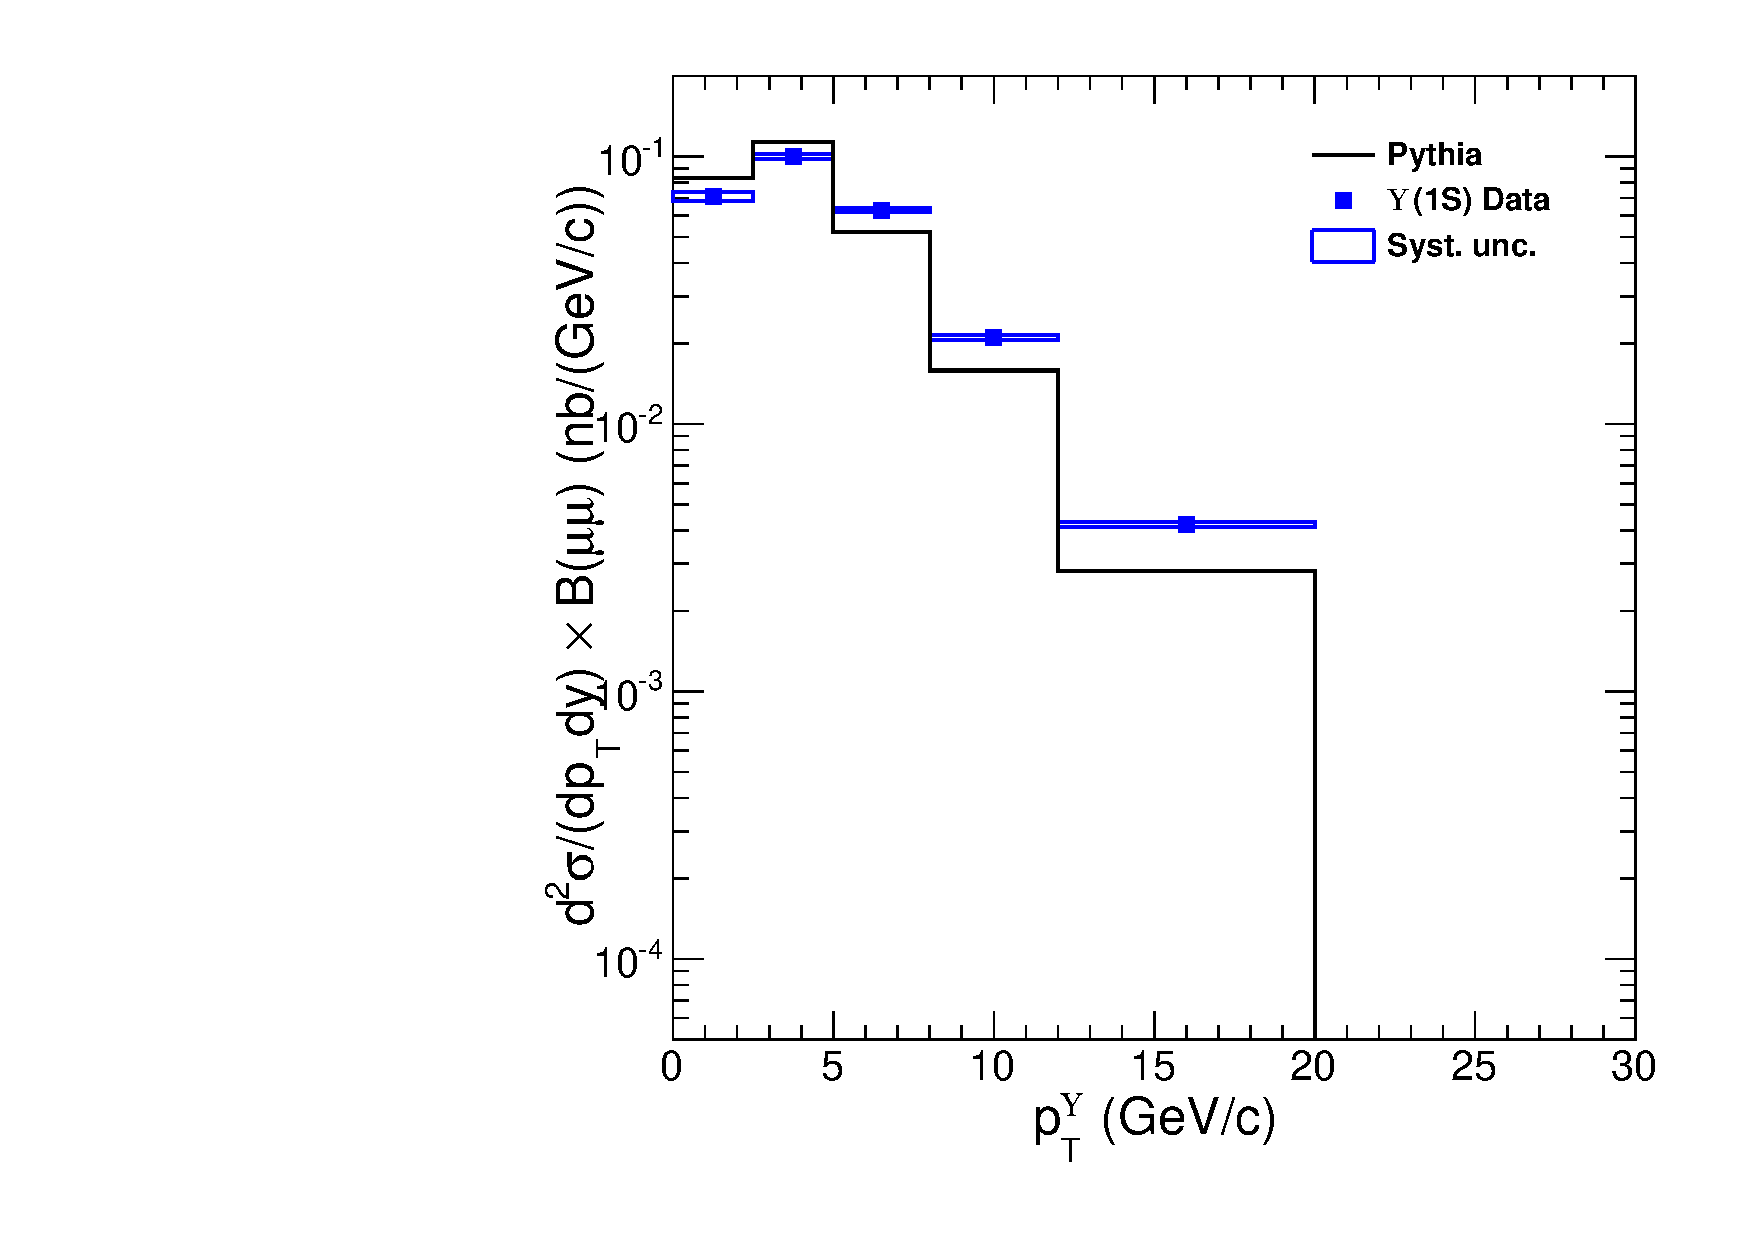
\includegraphics[width=0.49\textwidth]{Chapters/aCorrection/Y1Spt.pdf}
  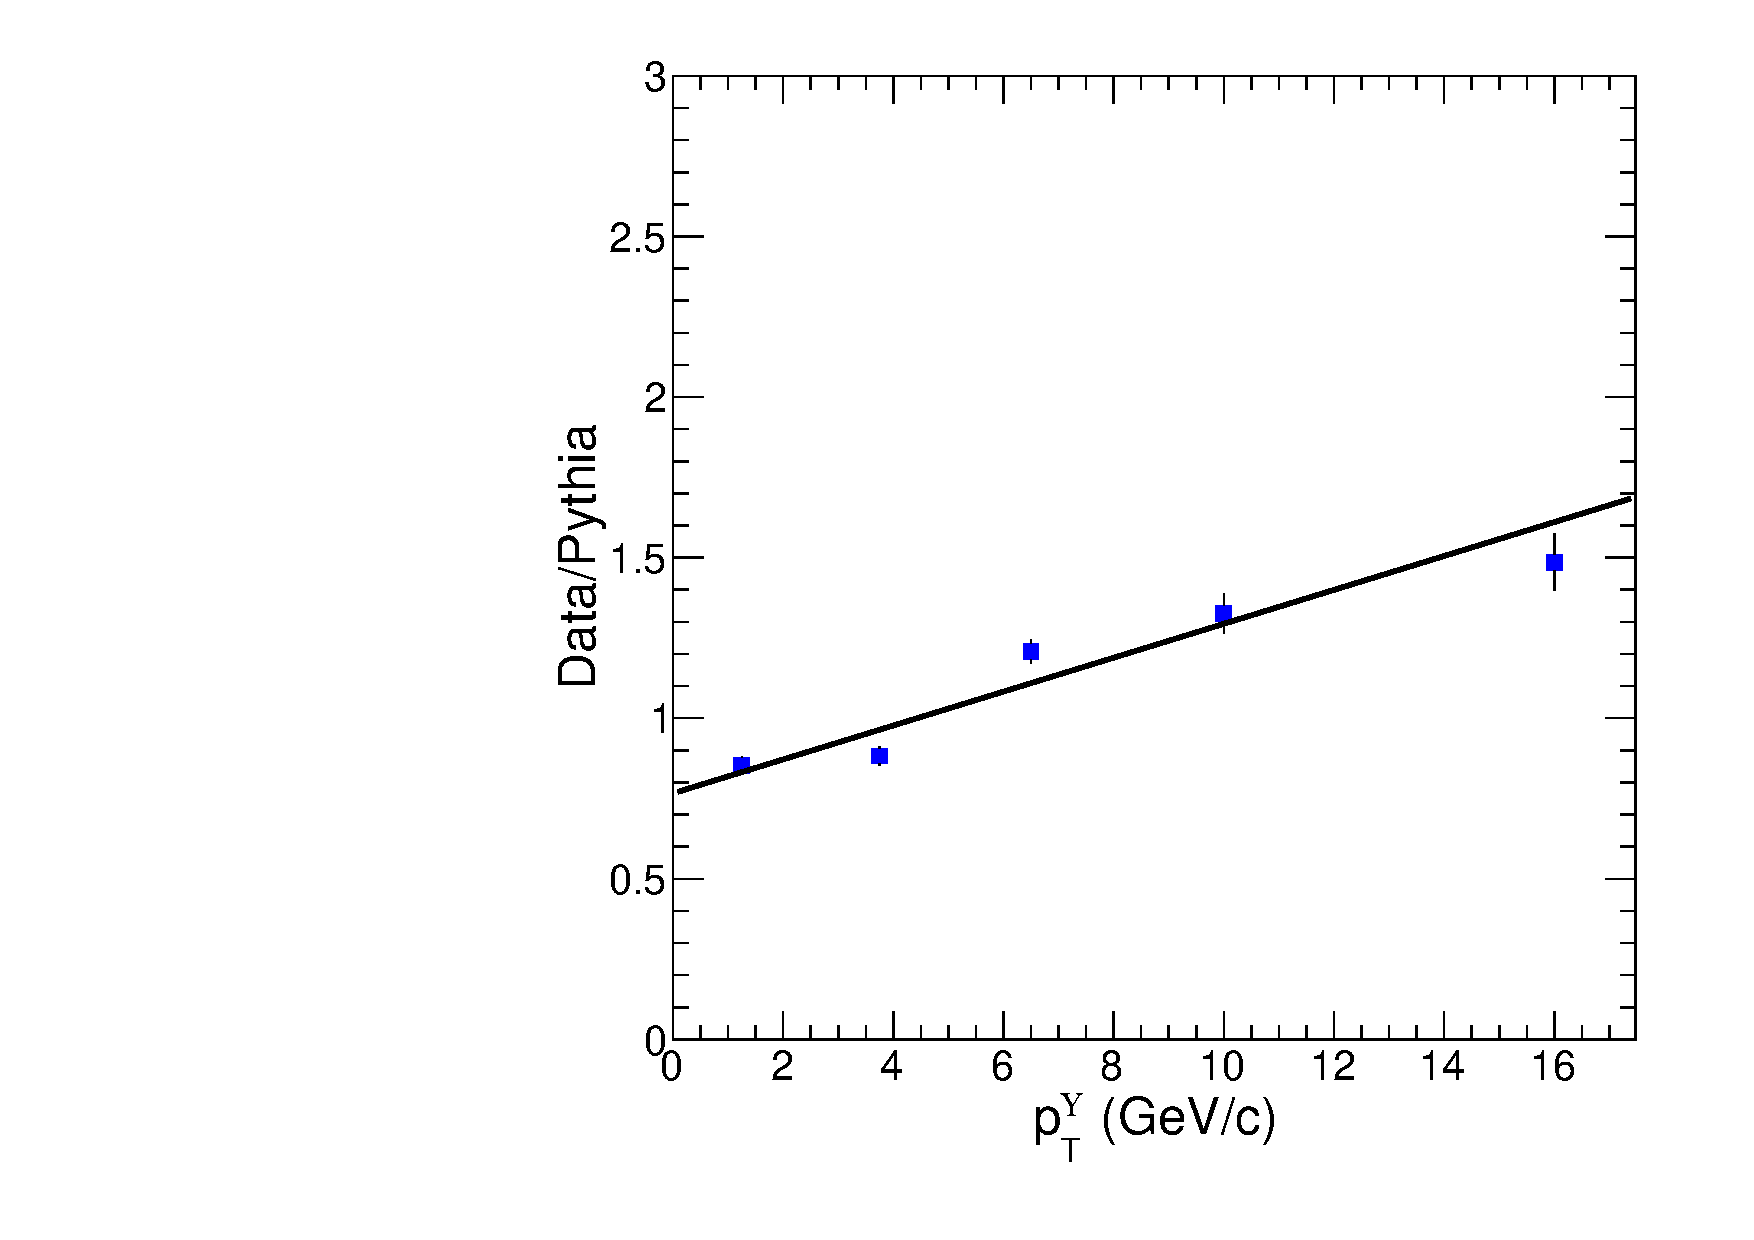
\includegraphics[width=0.49\textwidth]{Chapters/aCorrection/RaY1Spt.pdf}
  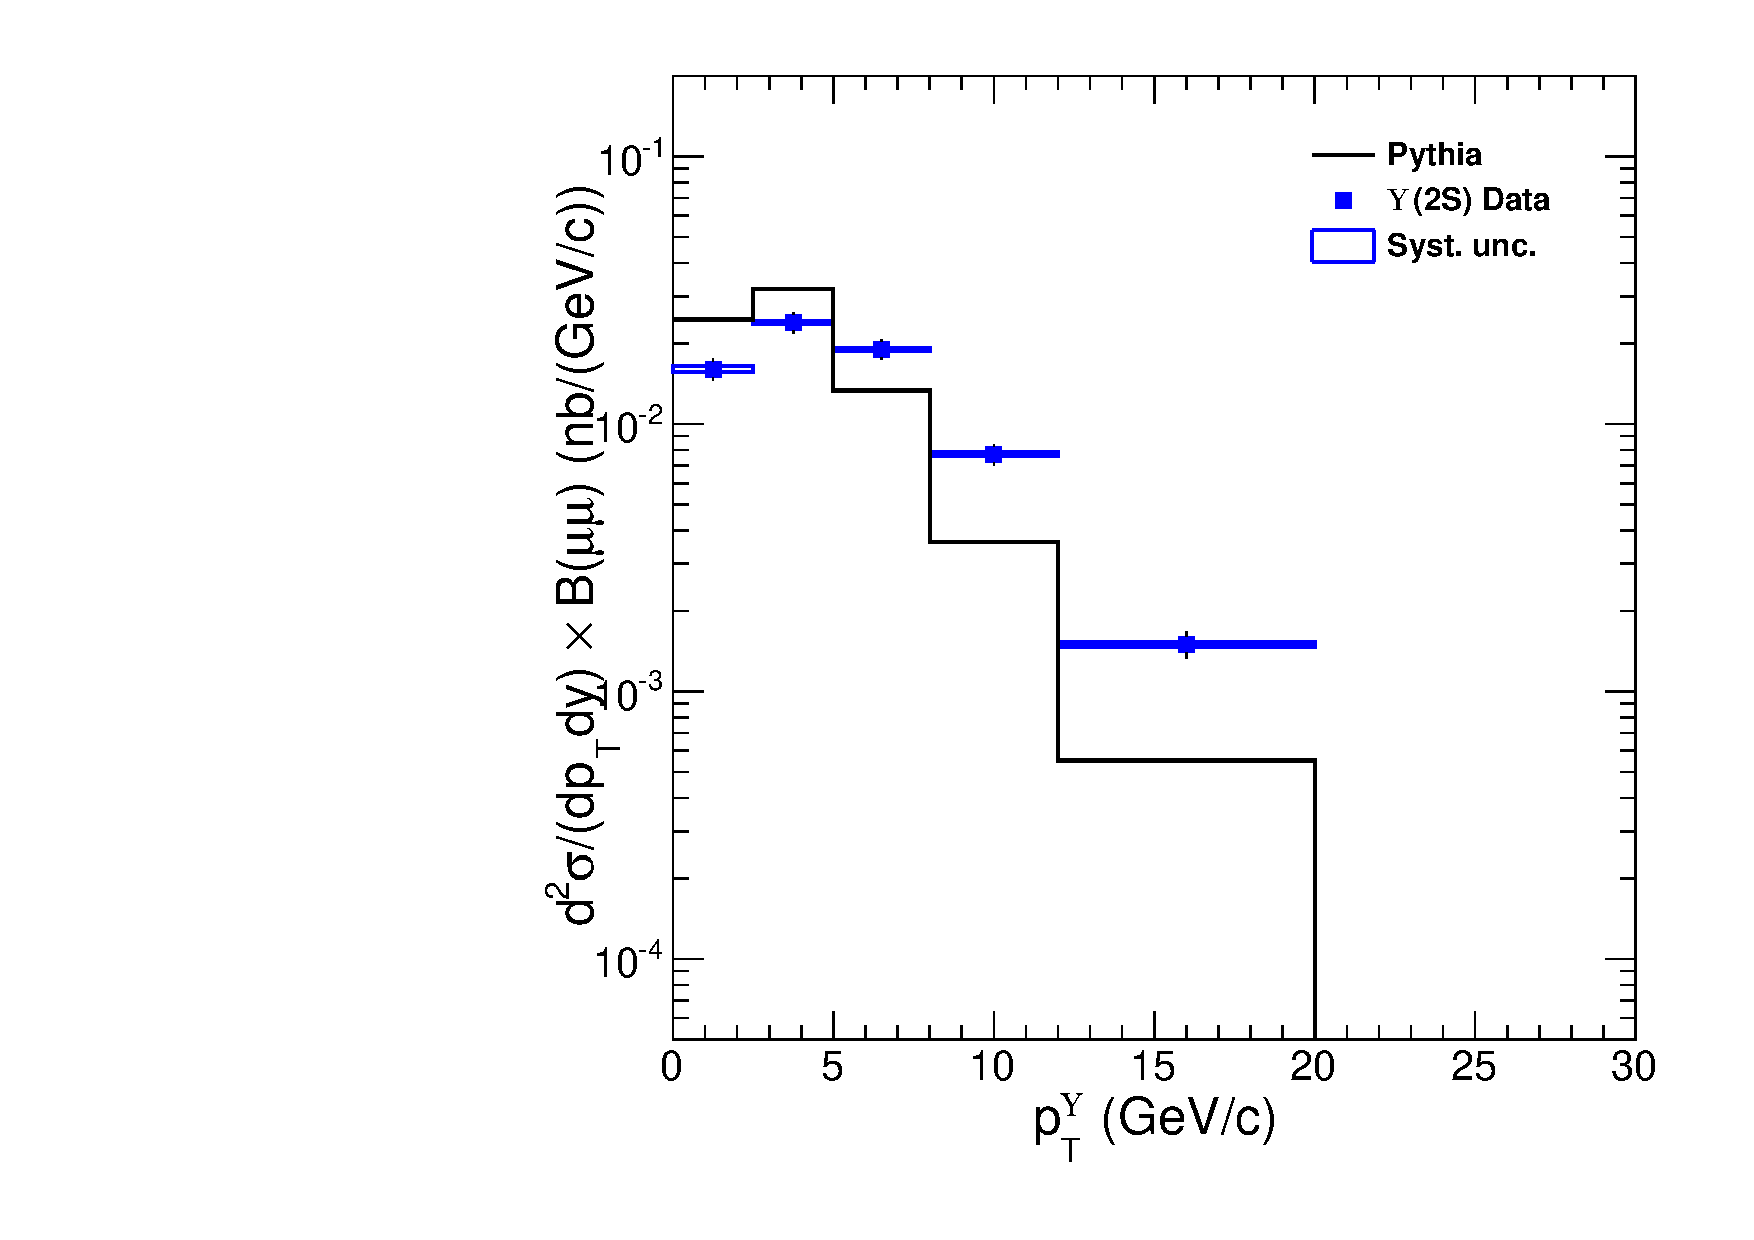
\includegraphics[width=0.49\textwidth]{Chapters/aCorrection/Y2Spt.pdf}
  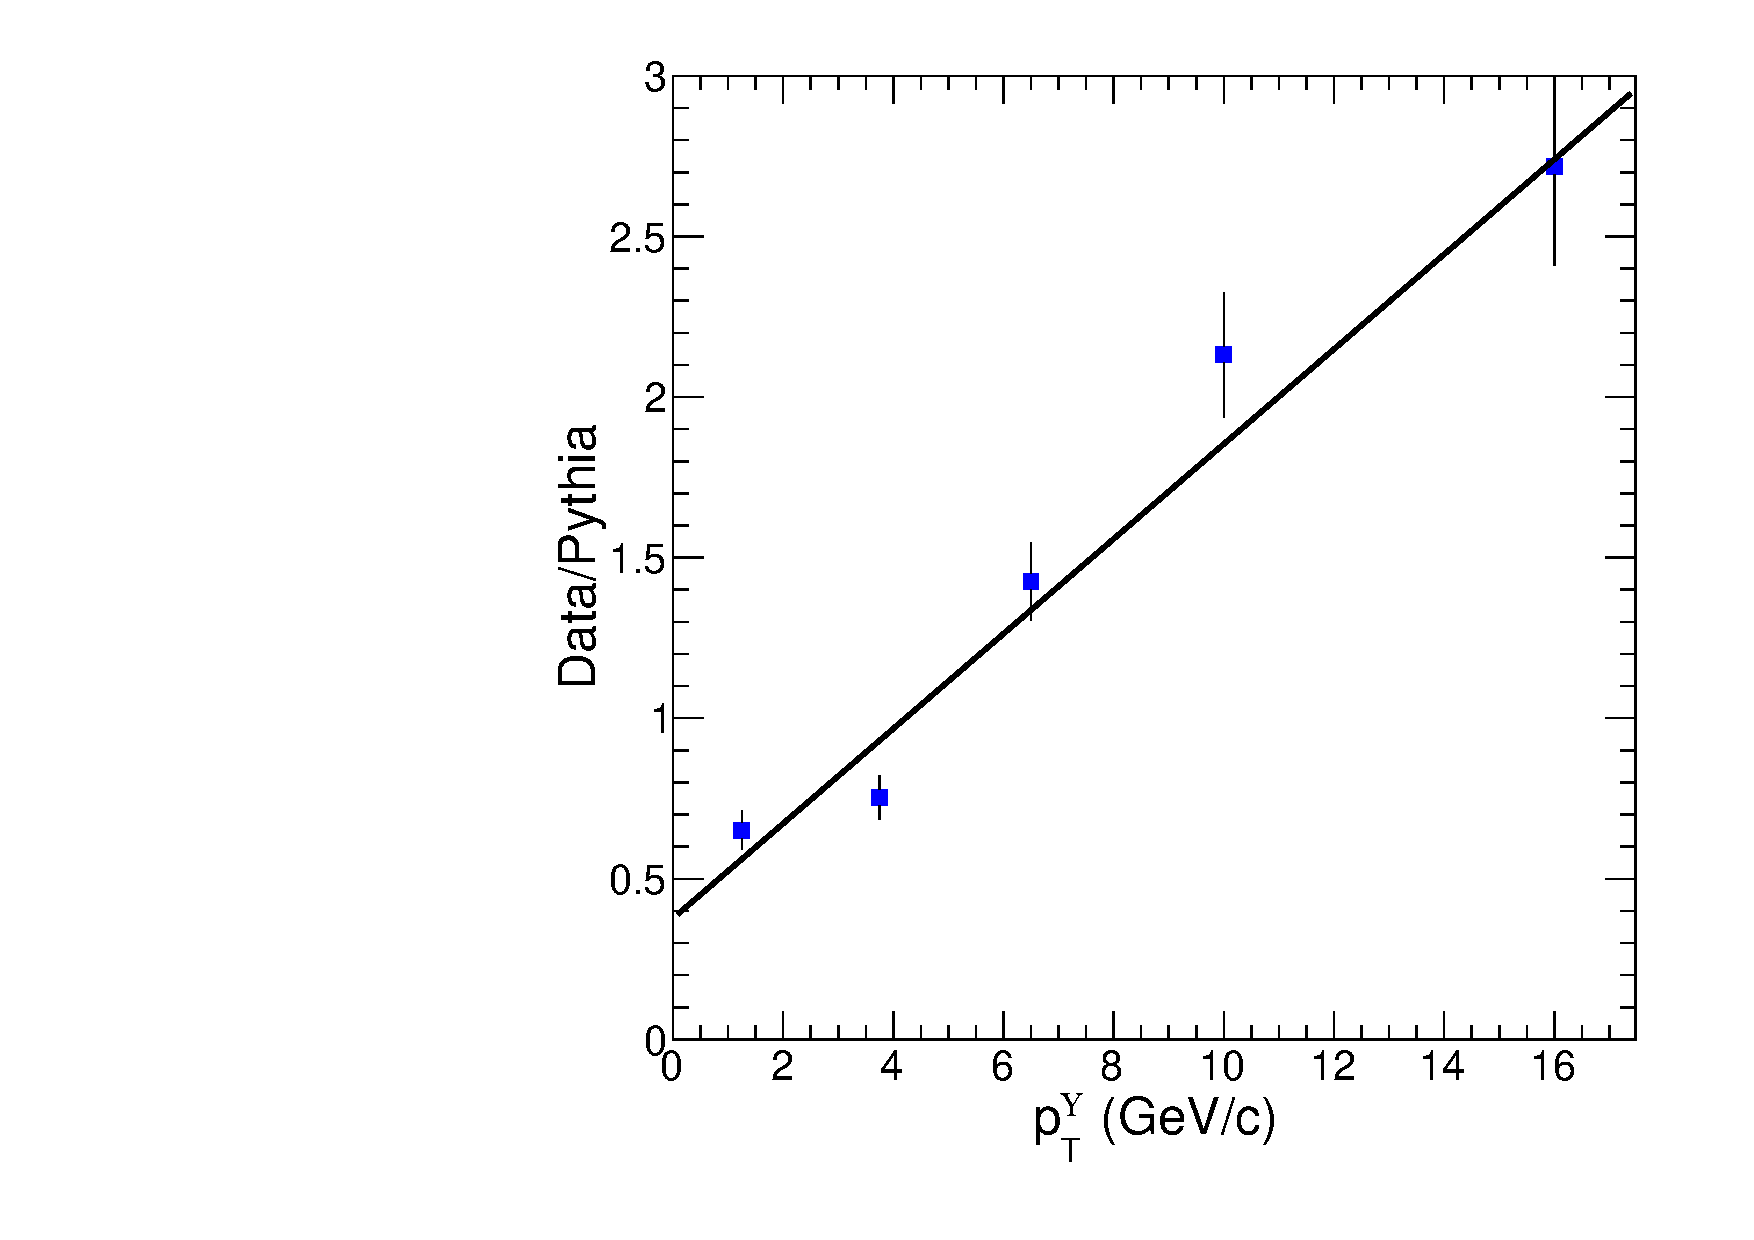
\includegraphics[width=0.49\textwidth]{Chapters/aCorrection/RaY2Spt.pdf}
  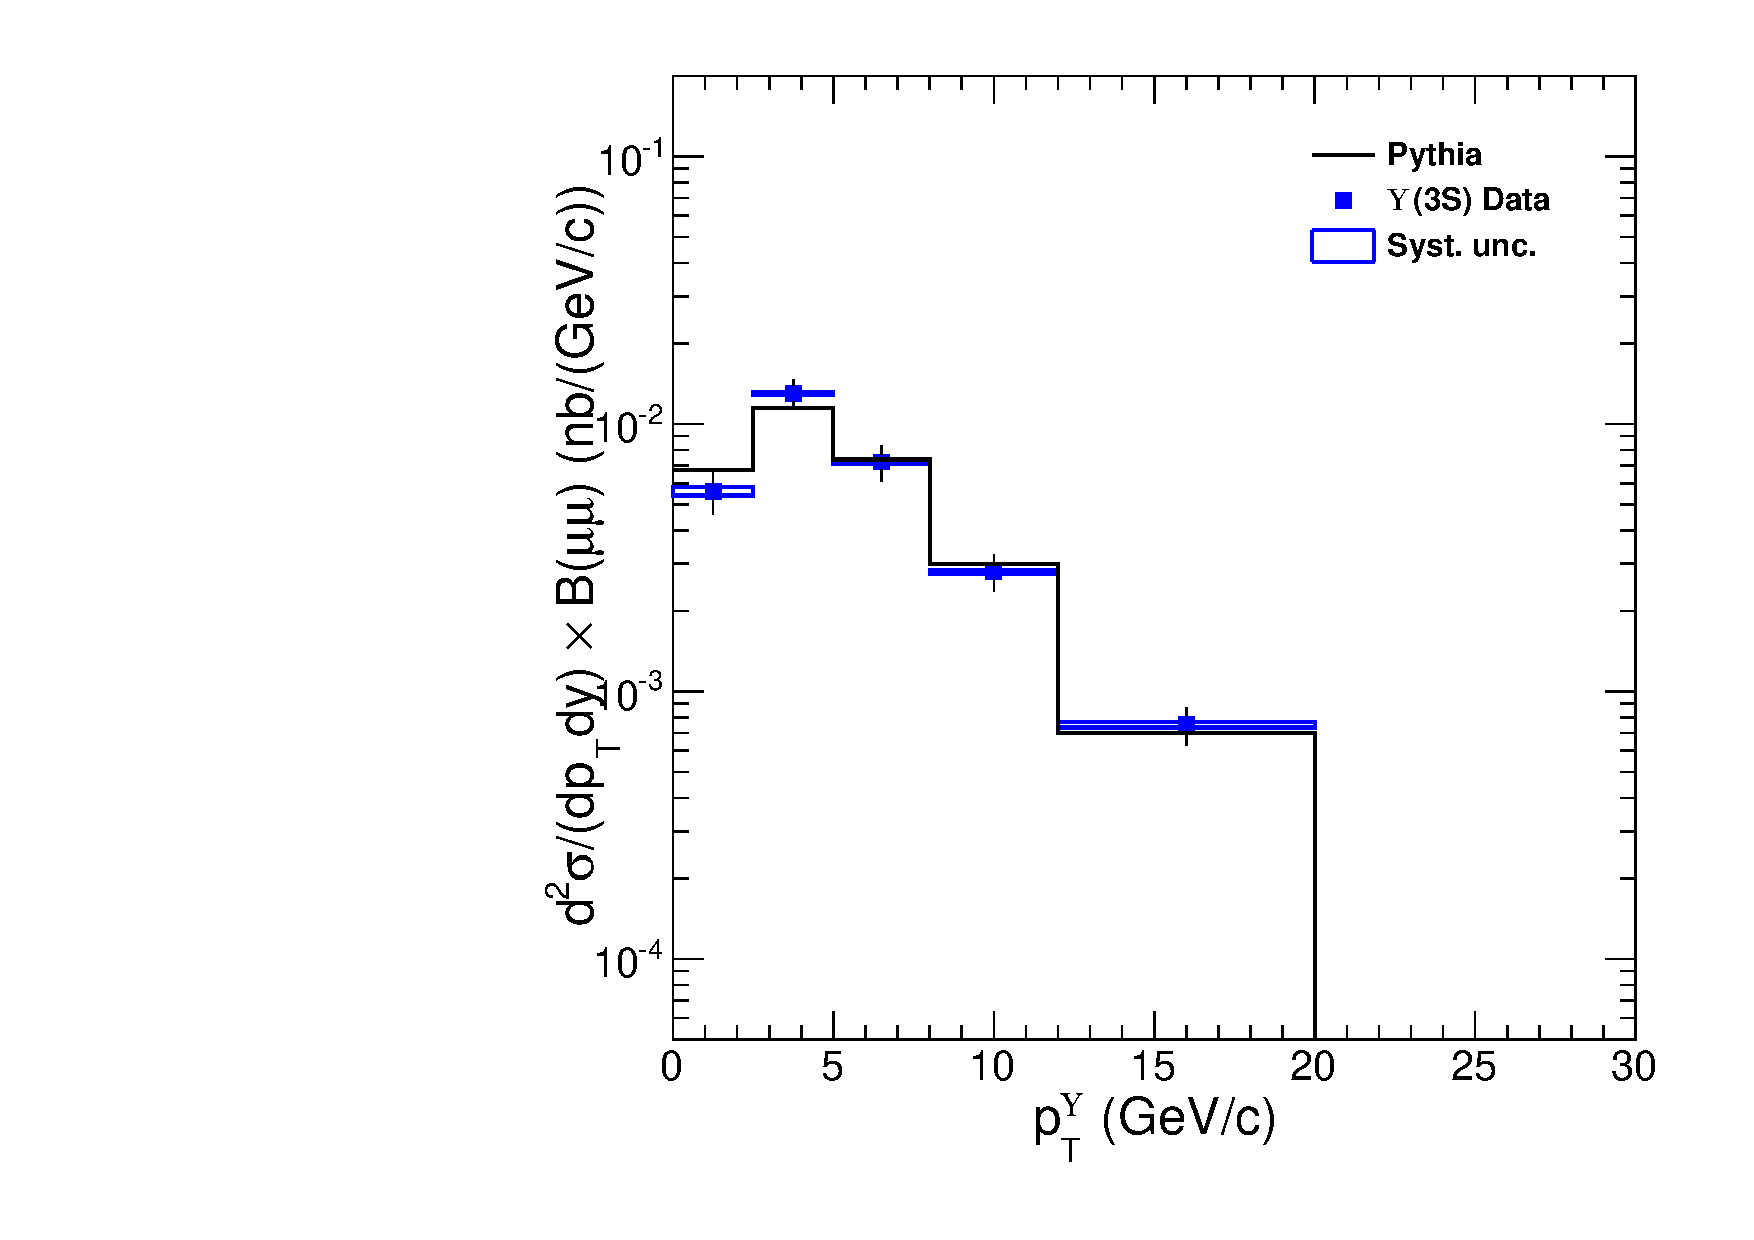
\includegraphics[width=0.49\textwidth]{Chapters/aCorrection/Y3Spt.pdf}
  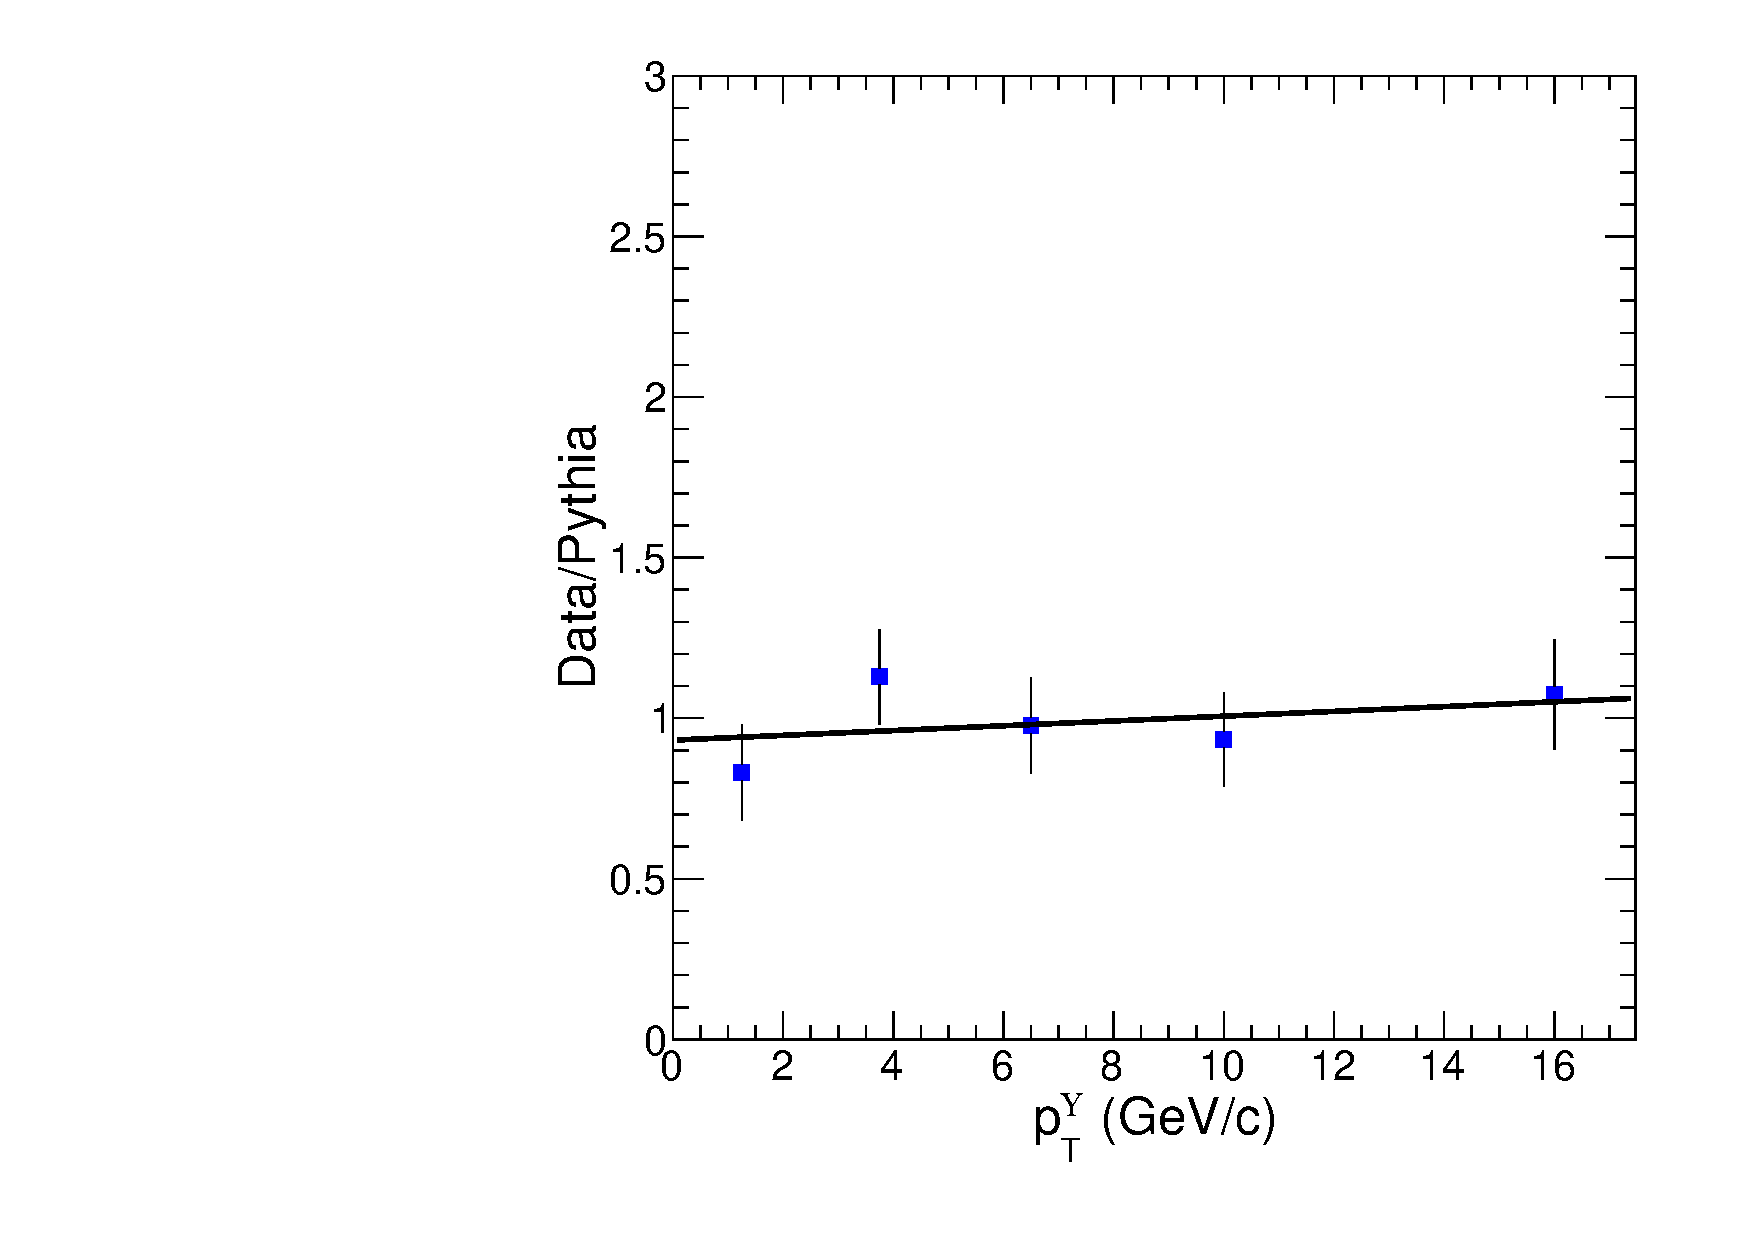
\includegraphics[width=0.49\textwidth]{Chapters/aCorrection/RaY3Spt.pdf}
  \caption{Left: \pt-spectrum of \PgU(nS) production measured in $pp$
    data at \s = 2.76 \TeV (blue
    squares), assumed by PYTHIA (histogram). Right: ratio of the two
    distributions Data/PYTHIA, fitted with a line to extract the
    weight functions $w_{n}(\pt)$.
    Top: \PgUa; Middle: \PgUb; Bottom: \PgUc.}
  \label{fig:pythia_data} 
\end{centering}  
\end{figure}

The reweighting functions $w_1$,~$w_2$~and $w_3$, that are applied to
\PgUa, \PgUb\ and \PgUc, are respectively defined in
Equations~\ref{eq:1sw} to~\ref{eq:3sw}

\begin{eqnarray}
\label{eq:1sw}
w_1(\pt) &=& 0.766 + 0.053*p_T^{\GEN}  \\ 
\label{eq:2sw}
w_2(\pt) &=& 0.377 + 0.148*p_T^{\GEN}   \\
\label{eq:3sw}
w_3(\pt) &=& 0.932 + 0.00745*p_T^{\GEN} 
\end{eqnarray}

After re-weighting the MC events used in acceptance and efficiency,
nominal acceptance and efficiency corrections were obtained (which are the ones I have presented above in
Sections~\ref{sec:acceptance},~\ref{sec:eff}). For the purpose of
estimating a systematic uncertainty accounting for the differences in
observed spectra, variations are performed by changing the slope
of $w_1$,~$w_2$~and $w_3$ by $\pm$20\%.

Changing the \pt\ slope of the weights by $\pm$20\% has an effect on the
\pt- and \y-dependence of \acc\eff, the product of acceptance and efficiency. To
extract a systematic uncertainty on \acc\eff\ from the slope variations, the maximum
deviations \vs. \pt and \vs. \y\ are used. % summed in quadrature.
In PbPb, an additional uncertainty source from the centrality
distribution is considered, which is reviewed next.

For the case of \PgUa, the nominal results for acceptance times
efficiency \vs. rapidity and \pt\ are presented in
Table~\ref{totalacceff} for $pp$ and Table~\ref{totalacceff_pbpb} for
PbPb. The statistical uncertainties displayed there are only related
to the size of the simulation samples. 

The systematic uncertainties \acc\eff$_{pp}$ presented in Table~\ref{totalacceff} for
pp have a relative size of $2 \sim 3$ \% for the \PgUa\
\pt-dependence, and $1 \sim 2$ \% for the \PgUa\ rapidity
dependence.

%Introduce the acc*eff of table 9(pp) and table (10), say that variations are taken as
%the max dev for pt and rap. Discuss the size of the systematic in the conclusion.
%The maximal deviation to the \pt-binned efficiencies of Table
% DO not forget, the results are on acc*eff, not eff alone!
%  The efficiencies are recomputed with the +20\% and
% -20\% variations on the \pt-weighting, and the maximum deviation with
% the nominal efficiency is taken as the uncertainty on the assumed \pt\
% spectrum.


%  Doing the same with the \y-dependent spectrum gives two
% other efficiencies, from which the maximum deviation with respect to
% the nominal efficiency is taken as the uncertainty on the assumed
% rapidity spectrum. These two uncertainties are summed in quadrature,
% along with the uncertainty on the assumed centrality distribution
% which I review next, to get a global systematic uncertainty
% for the dimuon efficiency.

\begin{table}[h]
\begin{center}
\begin{tabular}{|c|c||c|c|}
\hline
\pt [\GeVc]& \acc\eff$_{pp}$[1S](\pt)      & $\vert\y\vert$     &      \acc\eff$_{pp}$[1S](\y) \\
\hline                                       
0-2.5             & 0.301 $\pm$ 0.001 $\pm$0.008  & 0-0.4   &0.279 $\pm$ 0.002 $\pm$ 0.003  \\
2.5-5             & 0.193 $\pm$ 0.001 $\pm$0.004  & 0.4-0.8 &0.278 $\pm$ 0.002 $\pm$ 0.003  \\
5-8               & 0.190 $\pm$ 0.001 $\pm$0.006  & 0.8-1.2 &0.280 $\pm$ 0.002 $\pm$ 0.003  \\
8-12              & 0.267 $\pm$ 0.002 $\pm$0.008  & 1.2-1.6 &0.262 $\pm$ 0.002 $\pm$ 0.003  \\
12-20             & 0.388 $\pm$ 0.004 $\pm$0.012  & 1.6-2   &0.208
$\pm$ 0.001 $\pm$ 0.004  \\
\cline{1-2}
\textbf{0-100}             & \textbf{0.239 $\pm$ 0.001 $\pm$0.007}  & 2-2.4   &0.073 $\pm$ 0.001 $\pm$ 0.002  \\
\hline                           
\end{tabular}
\caption{Acceptance $\times$ efficiency for $\Upsilon$(1S) in the pp
  case. Listed uncertainties are first statistical from MC sample
  size, and systematic second. Integrated values are boldfaced.}
\label{totalacceff}
\end{center}
\end{table}


\subsubsection*{From the generated centrality distribution}
In PbPb, the centrality of the collision is used to characterise
experimentally the impact parameter between the two Pb ions. Because
of the high multiplicity in the final state, one must model
correctly how the event reconstruction chain performs with increasing
multiplicities, i.e. by measuring the efficiency as a function of the
centrality of the event. 

In order to do so, all \PgU\ events simulated with PYTHIA are embedded in a HYDJET
simulated event. HYDJET is a minimum bias event generator; as a
result, the distribution of generated events is uniform over all
centrality percentiles (we often say it is 'flat' in centrality).

However, the natural production rate of quarkonia in heavy ions is
\textit{not} uniform with centrality. Since quarkonium production is a
hard process, its rate scales (at first order) with the number of hard
nucleon-nucleon collisions. Therefore, embedding one \PgU\ event
in each HYDJET event breaks the \Ncoll-dependence usually observed in
hard processes. Measuring the efficiency of detecting \PgU\ with a
wrong centrality distribution would bias the result.

To mimick the true centrality distribution, the simulated \PgU\ are
reweighted to reflect to our best knowledge of the centrality
dependence. Indeed, if \PgU\ were not modified in heavy ions, we would
see a perfect \Ncoll\ scaling, which is not the case. 

The reweighting factor for each centrality bin is presented in
Equation~\ref{eq:centralityweighting}. It is the mean number of binary collisions for this
bin, multiplied by the measured suppression factor \RAA(\PgU(nS)) (obtained with a simple
\Ncoll\ weighting to the \PgU\ simulated distributions):

\begin{equation}
w(c_{0}\textrm{\%}\text{--} c_{1}\textrm{\%}) =\RAA(c_{0}\textrm{\%}\text{--}c_{1}\textrm{\%})\,
\frac{1}{c_{1}-c_{0}} \int_{c_{0}}^{c_{1}} \Ncoll \,\mathrm{d}c \equiv
\RAA(\textrm{bin})\langle \Ncoll (\textrm{bin}) \rangle,
\label{eq:centralityweighting}
\end{equation}

where $c_0$,~$c_1$ are the centrality percentiles of the bin
considered (e.g. 5\%--10\%).


Figure~\ref{fig:data_mc_cent} shows the centrality distributions for
events in data and MC, after applying the centrality weighting. % A slight

\begin{figure}[h]
\begin{centering}  
  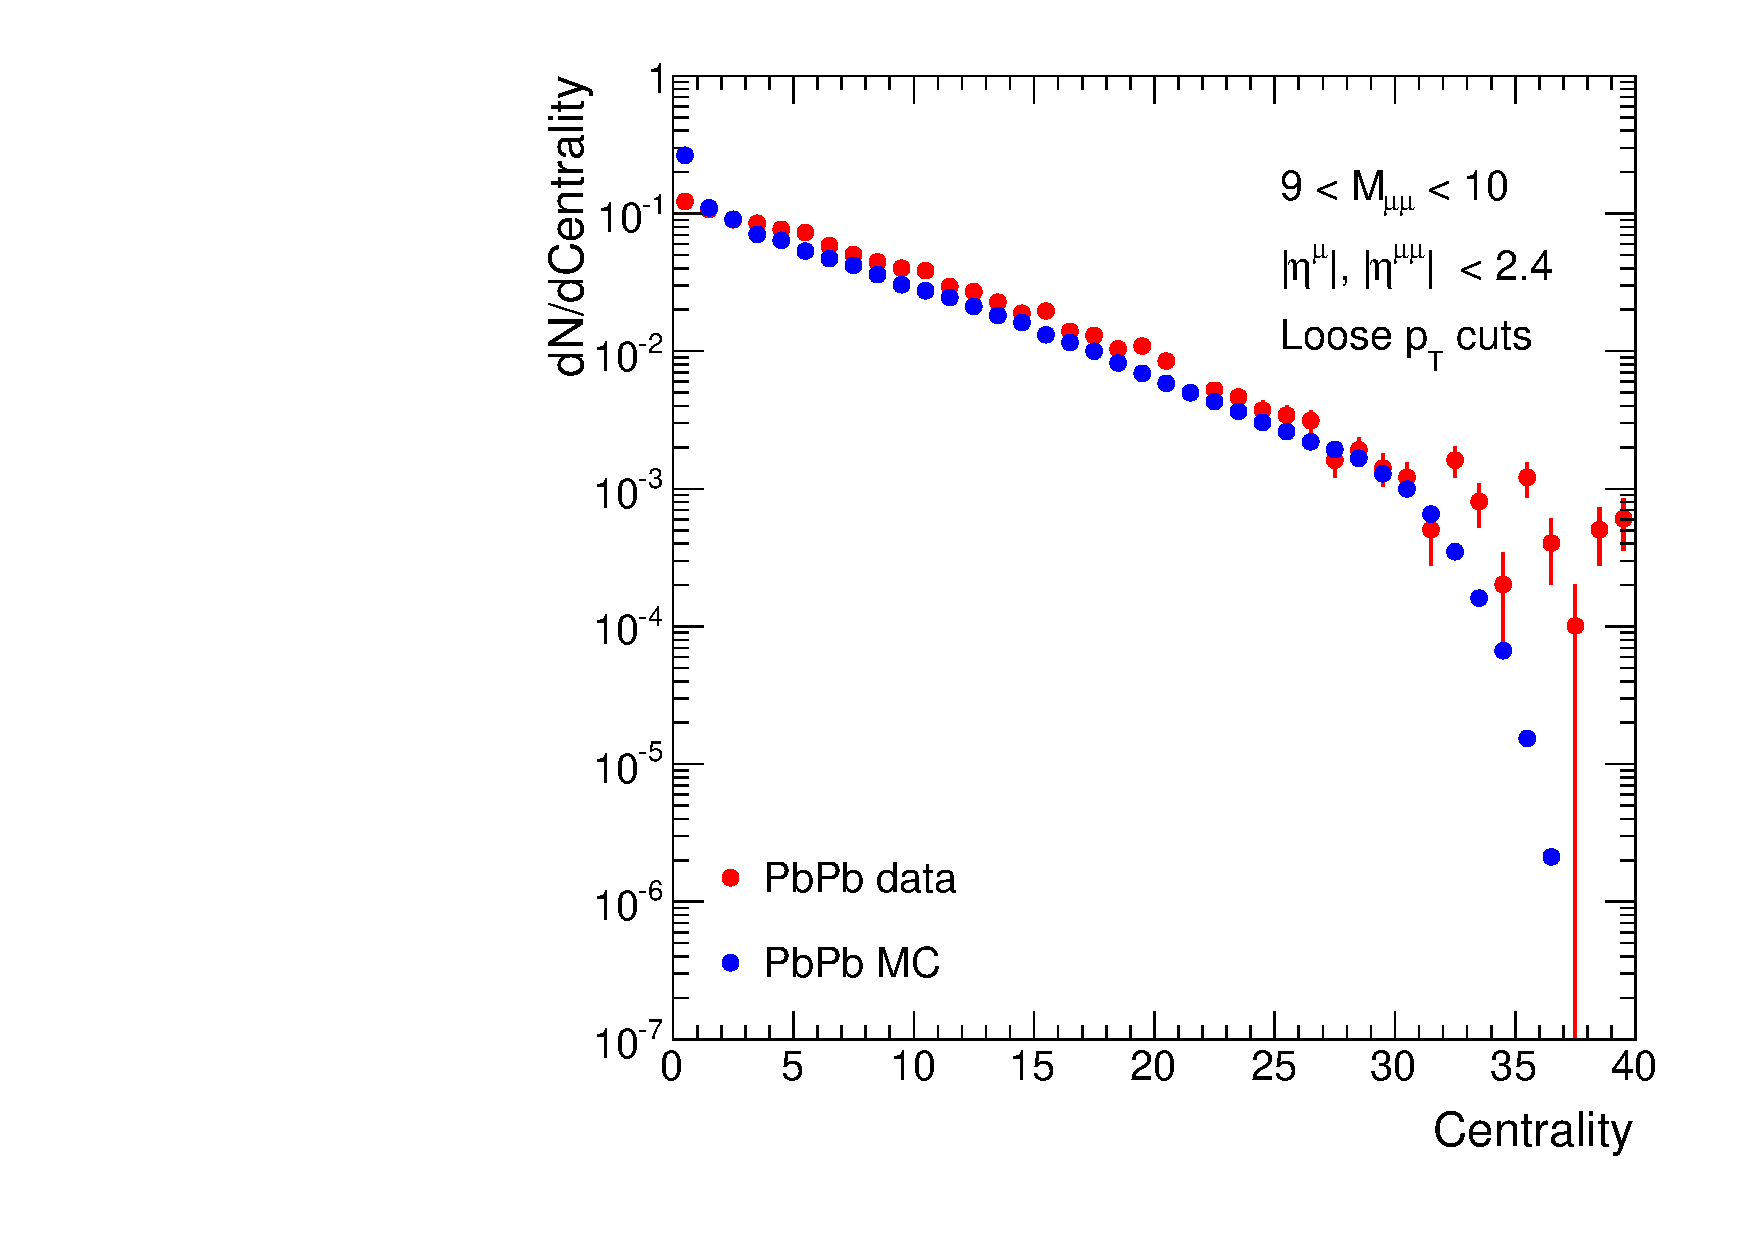
\includegraphics[width=0.6\textwidth]{Chapters/aCorrection/Centrality_PbPb_MC.pdf}
  \caption{Centrality distribution of dimuon candidates in the mass
    range of the \PgU\ measured in data (red), and \PgU\ generated
    with HYDJET, after \Ncoll\ weighting (blue). The x axis
    corresponds to generated centrality bins: each bin is 2.5\% of
    the centrality percentile table.}
  \label{fig:data_mc_cent}
\end{centering}  
\end{figure}
We cannot get rid of the \Ncoll\ weighting to get a
meaningful centrality distribution. Otherwise, the (red) MC
distribution would look rather flat, and bias the efficiency.

Efficiencies are computed with the centrality reweighting, and compared to the
efficiencies obtained with a simpler weighting of \Ncoll, that is,
setting \RAA\ to 1 in Equation~\ref{eq:centralityweighting}. The systematic uncertainty
from this procedure is taken as the difference between the two
efficiencies. The total \PgUa\ \acc~$\times$~\eff\ systematic
uncertainties are obtained by summing in quadrature this uncertainty
and the two uncertainties from
shifting the shapes \vs. \pt\ and \y. 

The total \PgUa\ \acc~$\times$~\eff\ with the systematic uncertainties 
are presented in Table~\ref{totalacceff_pbpb} for PbPb
efficiencies. Because the \pt\ and rapidity spectra came from PYTHIA,
the effect of shifting the kinematics of the \PgU\ is of the same order
as what was seen in the previous paragraph for $pp$. However, the relative size of the
uncertainties appear larger in PbPb, of the order of $7 - 10$ \%, which is due to the
centrality re-weighting procedure. In other words, the uncertainty on
the assumed centrality distribution for \PgU\ is dominating the
systematic uncertainties on \acc\eff\ in PbPb.

\begin{table}[t]
\begin{center}
\begin{tabular}{|c|c||c|c|}
\hline
\pt [\GeVc]& \acc\eff[1S](\pt)      & |\y|     &      \acc\eff[1S](\y) \\
% \hline
% 0.000-5.000     &0.357 $\pm$ 0.001   &  \\
% 5.000-12.000    & 0.309 $\pm$ 0.001  &  \\
% 12.000-20.000   & 0.513 $\pm$ 0.005  &  \\
\hline                                       
0-2.5             &0.269 $\pm$ 0.002  $\pm$ 0.022  & 0-0.4   &0.240 $\pm$ 0.002  $\pm$ 0.012   \\
2.5-5             &0.175 $\pm$ 0.002  $\pm$ 0.013  & 0.4-0.8 &0.250 $\pm$ 0.002  $\pm$ 0.012  \\
5-8               &0.181 $\pm$ 0.002  $\pm$ 0.012  & 0.8-1.2 &0.265 $\pm$ 0.003  $\pm$ 0.014  \\
8-12              &0.266 $\pm$ 0.003  $\pm$ 0.016  & 1.2-1.6 &0.255 $\pm$ 0.003  $\pm$ 0.019  \\
12-20             &0.387 $\pm$ 0.004  $\pm$ 0.020  & 1.6-2   &0.206
$\pm$ 0.003  $\pm$ 0.025  \\
\cline{1-2}
\textbf{0-100}             &\textbf{0.223 $\pm$ 0.001  $\pm$ 0.015}  & 2-2.4   &0.076 $\pm$ 0.002  $\pm$ 0.011  \\
\hline                          
\end{tabular}
\begin{tabular}{|c|c|}
\hline
Centrality & \acc\eff[1S](Cent.)$_{\rm PbPb}$ \\
\hline
0\%-5\%   &0.214 $\pm$ 0.002  $\pm$  0.015 \\
5\%-10\%  &0.221 $\pm$ 0.003  $\pm$  0.015 \\
10\%-20\% &0.224 $\pm$ 0.002  $\pm$  0.016 \\
20\%-30\% &0.228 $\pm$ 0.002  $\pm$  0.016 \\
30\%-40\% &0.229 $\pm$ 0.002  $\pm$  0.016 \\
40\%-50\% &0.230 $\pm$ 0.002  $\pm$  0.016 \\
50\%-70\% &0.232 $\pm$ 0.002  $\pm$  0.016 \\
70\%-100\%&0.231 $\pm$ 0.002  $\pm$  0.016 \\
\hline                           
\end{tabular}
\caption{Acceptance $\times$ efficiency for $\Upsilon$(1S) in the PbPb
  case. Top: tables for \pt- and \y-binned efficiencies. Bottom:
  Centrality-binned efficiencies. Listed uncertainties are statistical
  first and systematic second.}
\label{totalacceff_pbpb}
\end{center}
\end{table}

\vspace{0.3cm}
\fbox{
  \parbox{0.9\textwidth}
  {\textsf{In this section, I have presented the first-order corrections applied
      to our extracted raw yields to evaluate the loss due to analysis cuts
      and detector inefficiencies. In the process, I have argued that \acc\eff\ could be seen as the transfer function between the
      physical yield and the experimental measurement. This 
      assumes that all sources of inefficiency (trigger,
      identification, etc.) are properly decscribed by Monte Carlo
      simulations. The next section details how this assumption is checked.}
  }
}

%  There are two crucial
% underlying assumptions here. The first assumption is, from the two muons reconstructed in the
% detector, that the association is well done and does not affect the
% dimuon efficiency, so that formally \eff(\PgU) = \eff($\mu_1$)~$\times$~\eff($\mu_2$). The second
% assumption is that our simulation of the detector and of its
% performance in reconstructing muons, is strictly the actual
% one. Unfortunately, we cannot follow the same strategy as in this
% section if we want to computed data-driven efficiencies. The next
% section details how this is done.




\clearpage
\section{Data-driven corrections and comparison to simulation}
\label{sec:data_mc}
\subsection{Data-MC comparisons of muon kinematics}
\label{sec:data_mc_kinematics}
First, let us look at the kinematics of the muons produced in our
collisions, and compare to what is obtained in the simulated
samples.%  If the most simple distributions (muon $\phi$, $\eta$, \pt)
% are not similar in MC and data, this means another re-weighting may be
% necessary. 

Figure~\ref{phi,eta} has the distributions for single muons
from the mass region of the \PgU, for data and MC. One can see that
within the statistical accuracy of the data, the distributions for
$\phi$ and $\eta$ are in a fairly good agreement.

% Section~\ref{subsec:centbins}.
\begin{figure}[h]
\begin{centering}  
  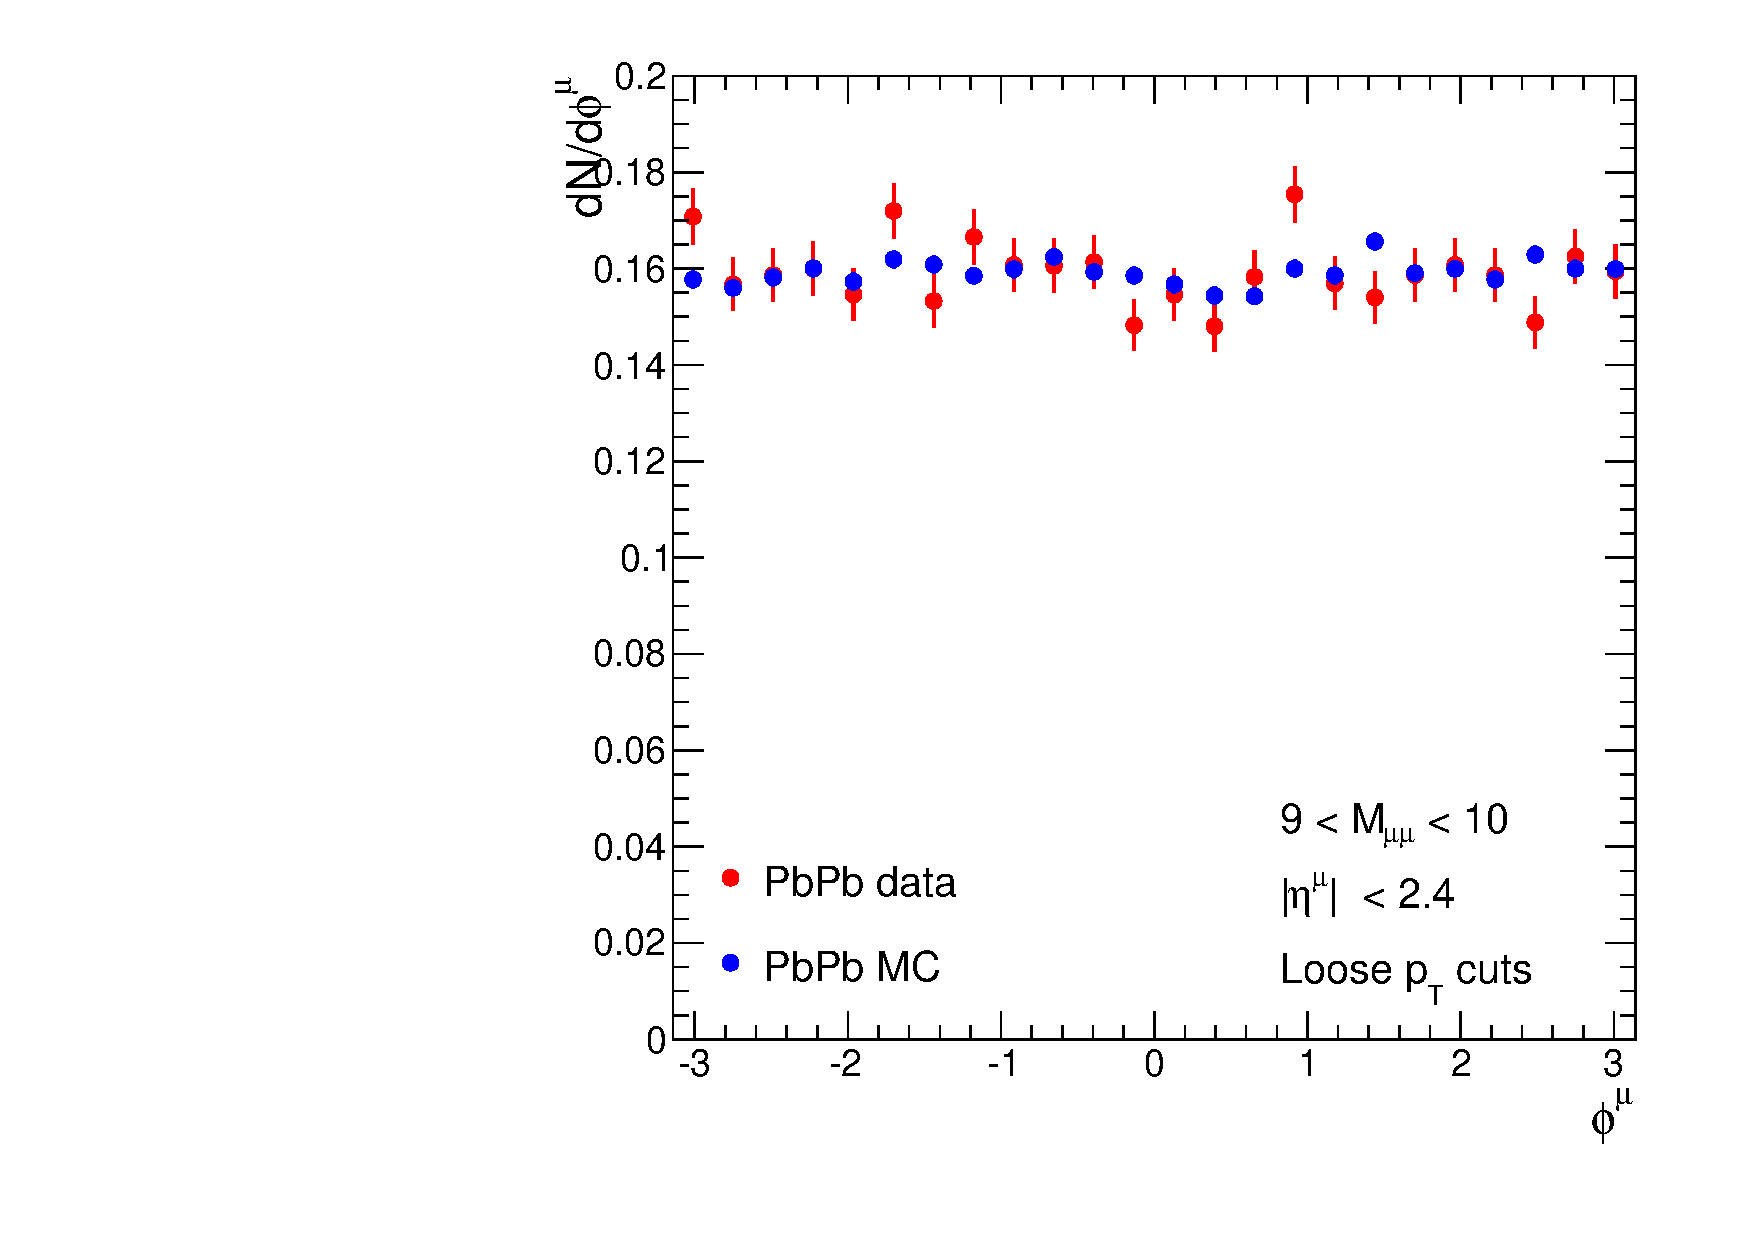
\includegraphics[width=0.49\textwidth]{Chapters/aCorrection/phi_aa_MC.pdf}
  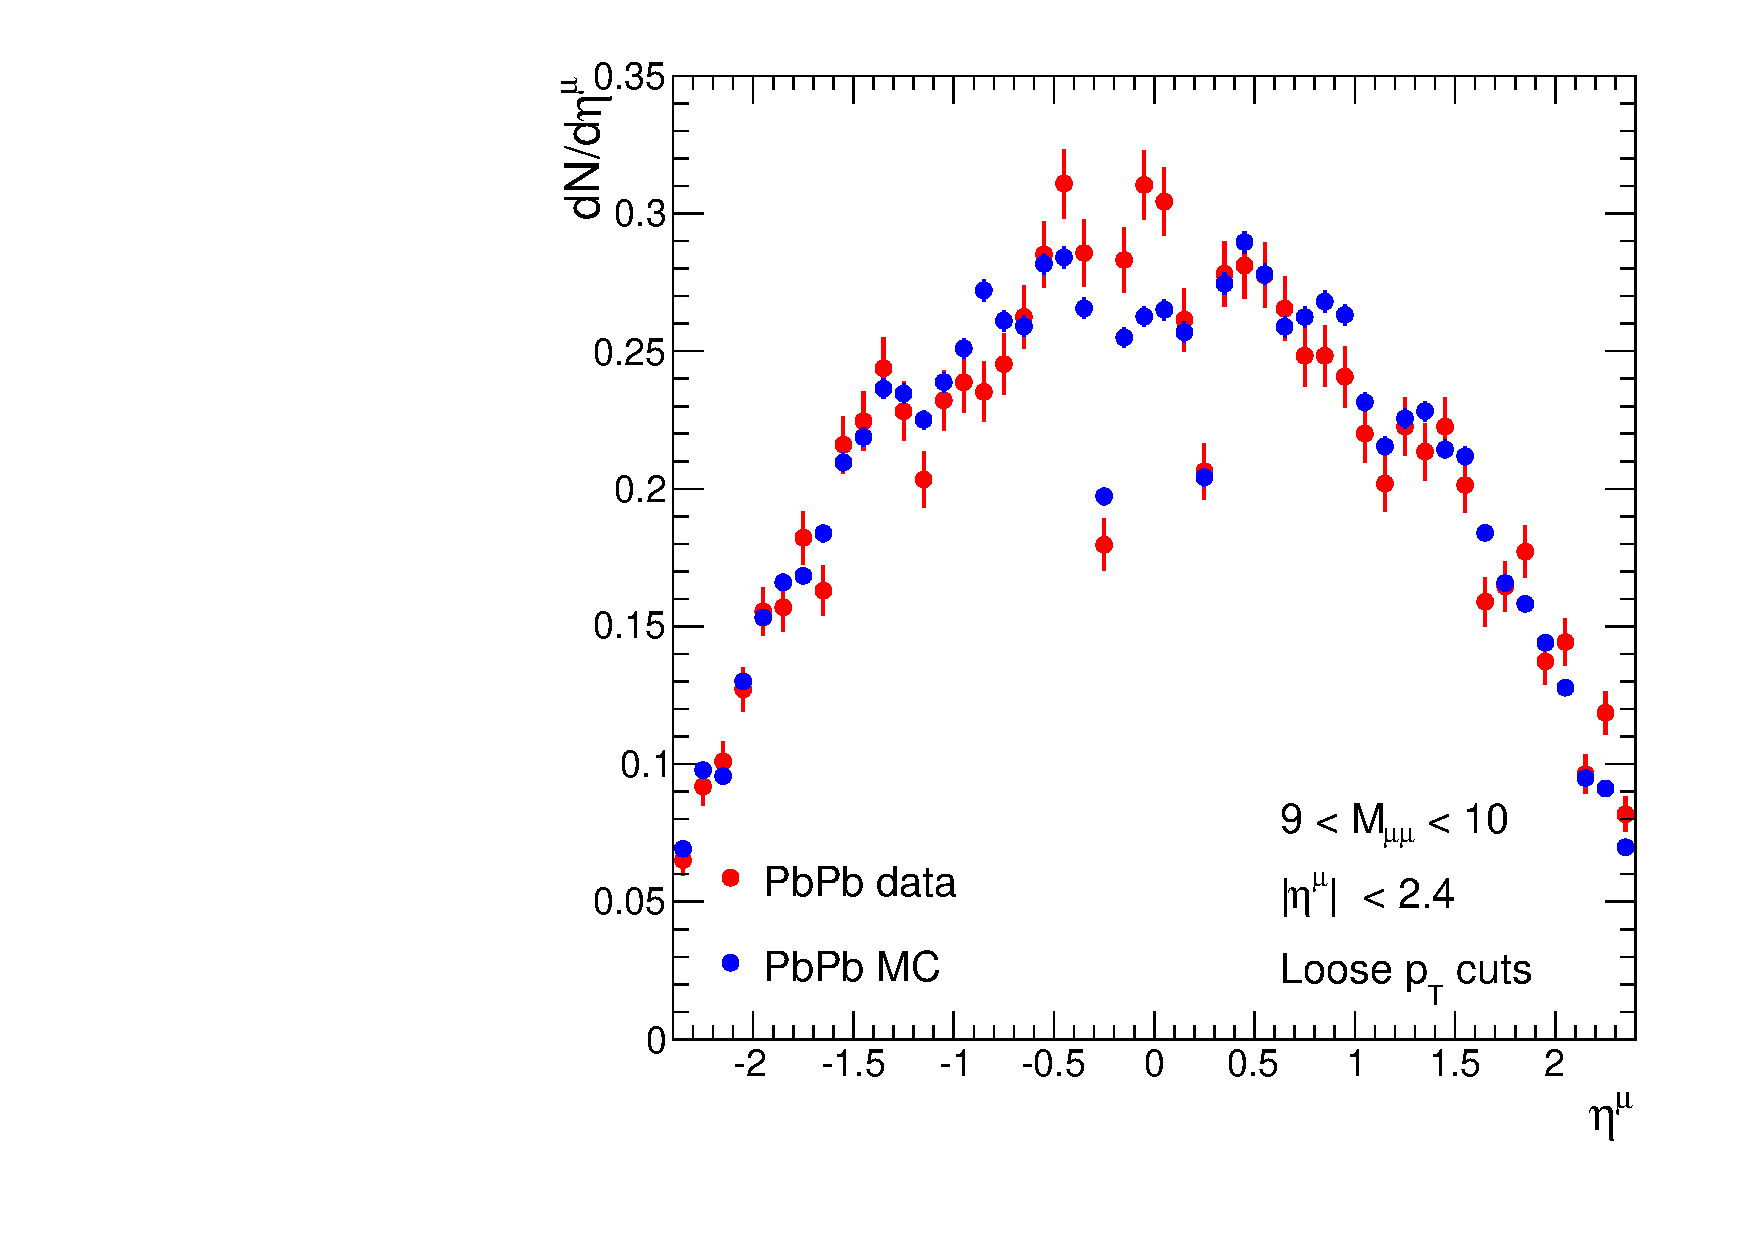
\includegraphics[width=0.49\textwidth]{Chapters/aCorrection/eta_aa_MC.pdf}
  \caption{Left: azimuthal $\phi$ distribution of single muons from pairs in the mass
    region of the \PgU. Right: pseudorapidity distribution of single muons from pairs in the mass
    region of the \PgU. Generated \PgU\ are in blue, and red is used
    for data.
  }
  \label{phi,eta}
\end{centering}  
\end{figure}

The single muon \pt\ distributions are worth looking at as
well. Since the collision data has signal and background, the \pt\
distribution for single muons is expected to be a mix of muons coming
from \PgU, and muons coming from the background. Consequently, the
\pt\ distributions will not coincide automatically, and a proper
comparison can only be done by looking at background subtracted
data. Figure~\ref{fig:pt_mcdata} (left) shows the single muon
distributions in data and MC before background subtraction.

\begin{figure}[h]
\begin{centering}  
  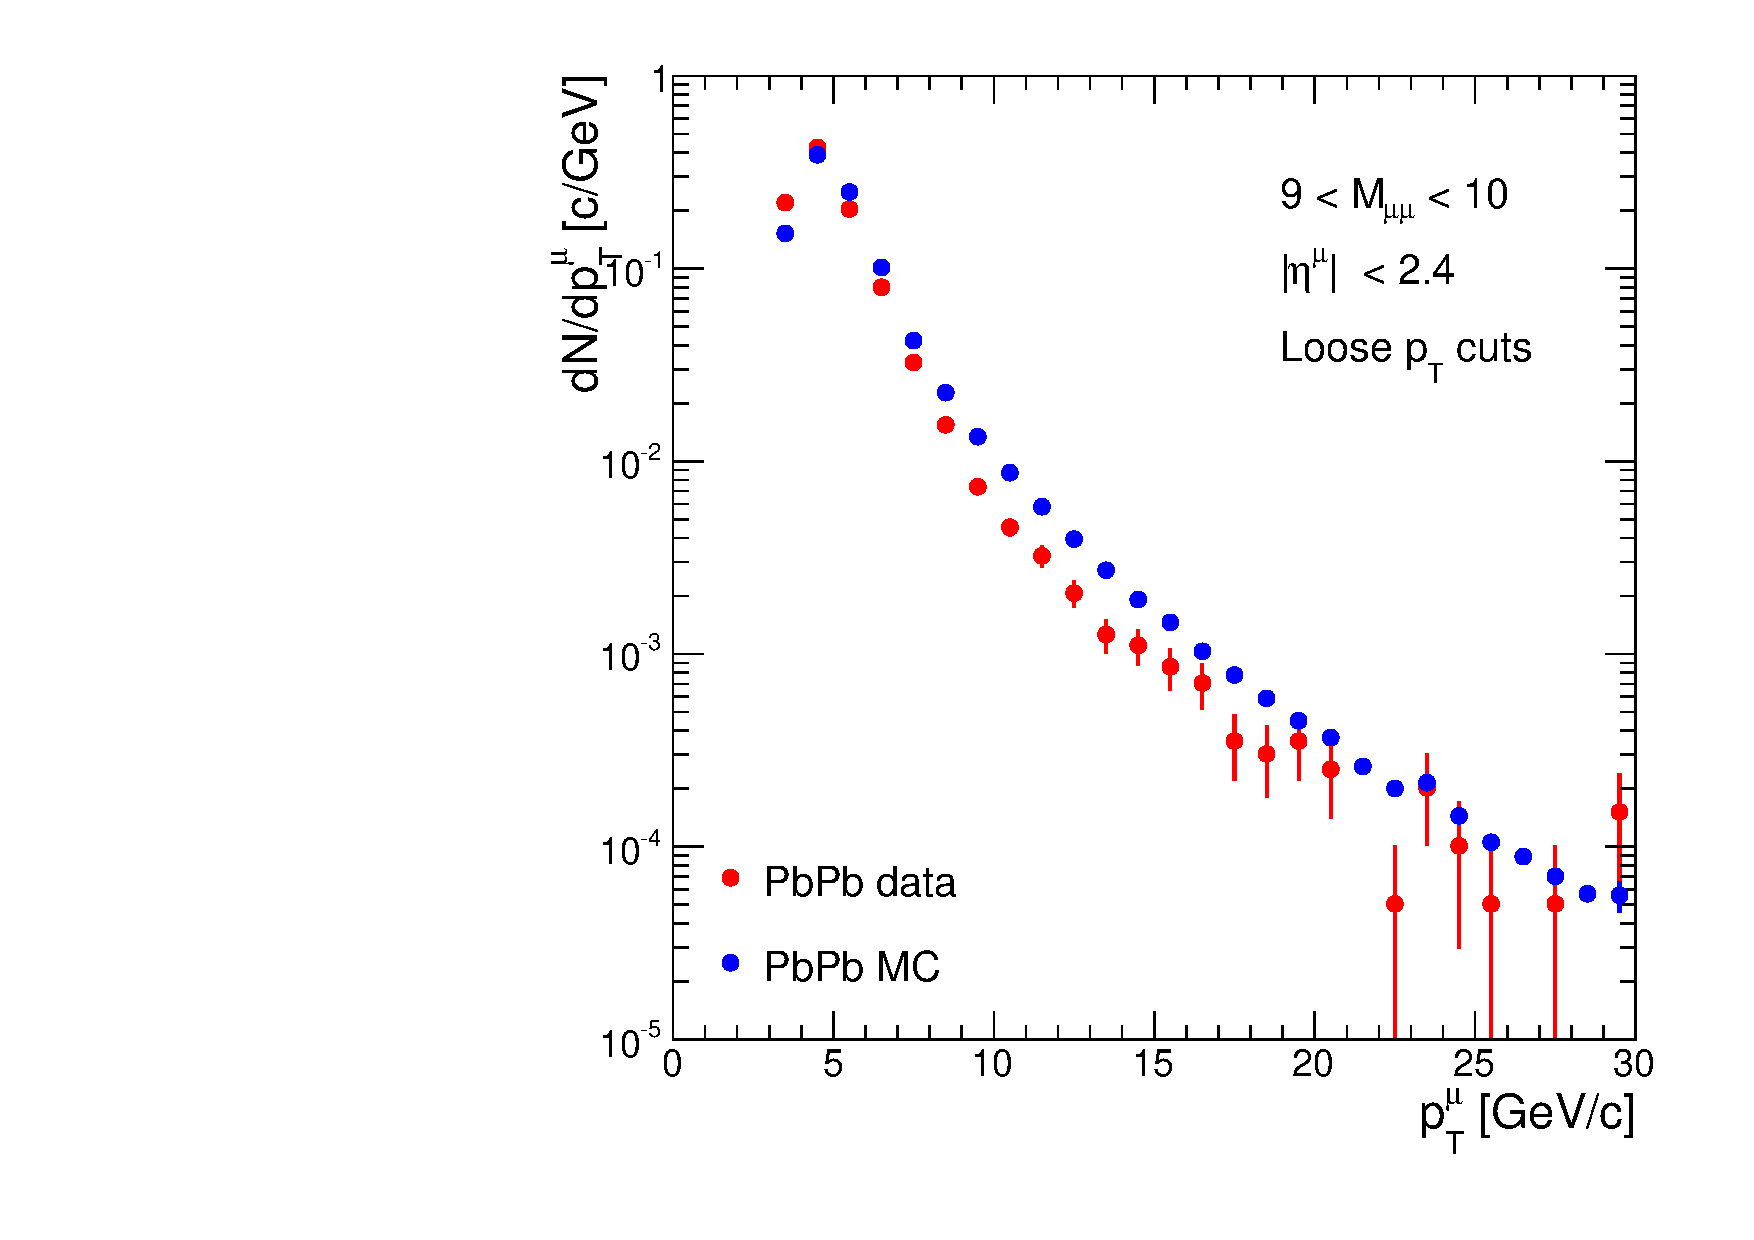
\includegraphics[width=0.49\textwidth]{Chapters/aCorrection/pt_aa_MC.pdf}
  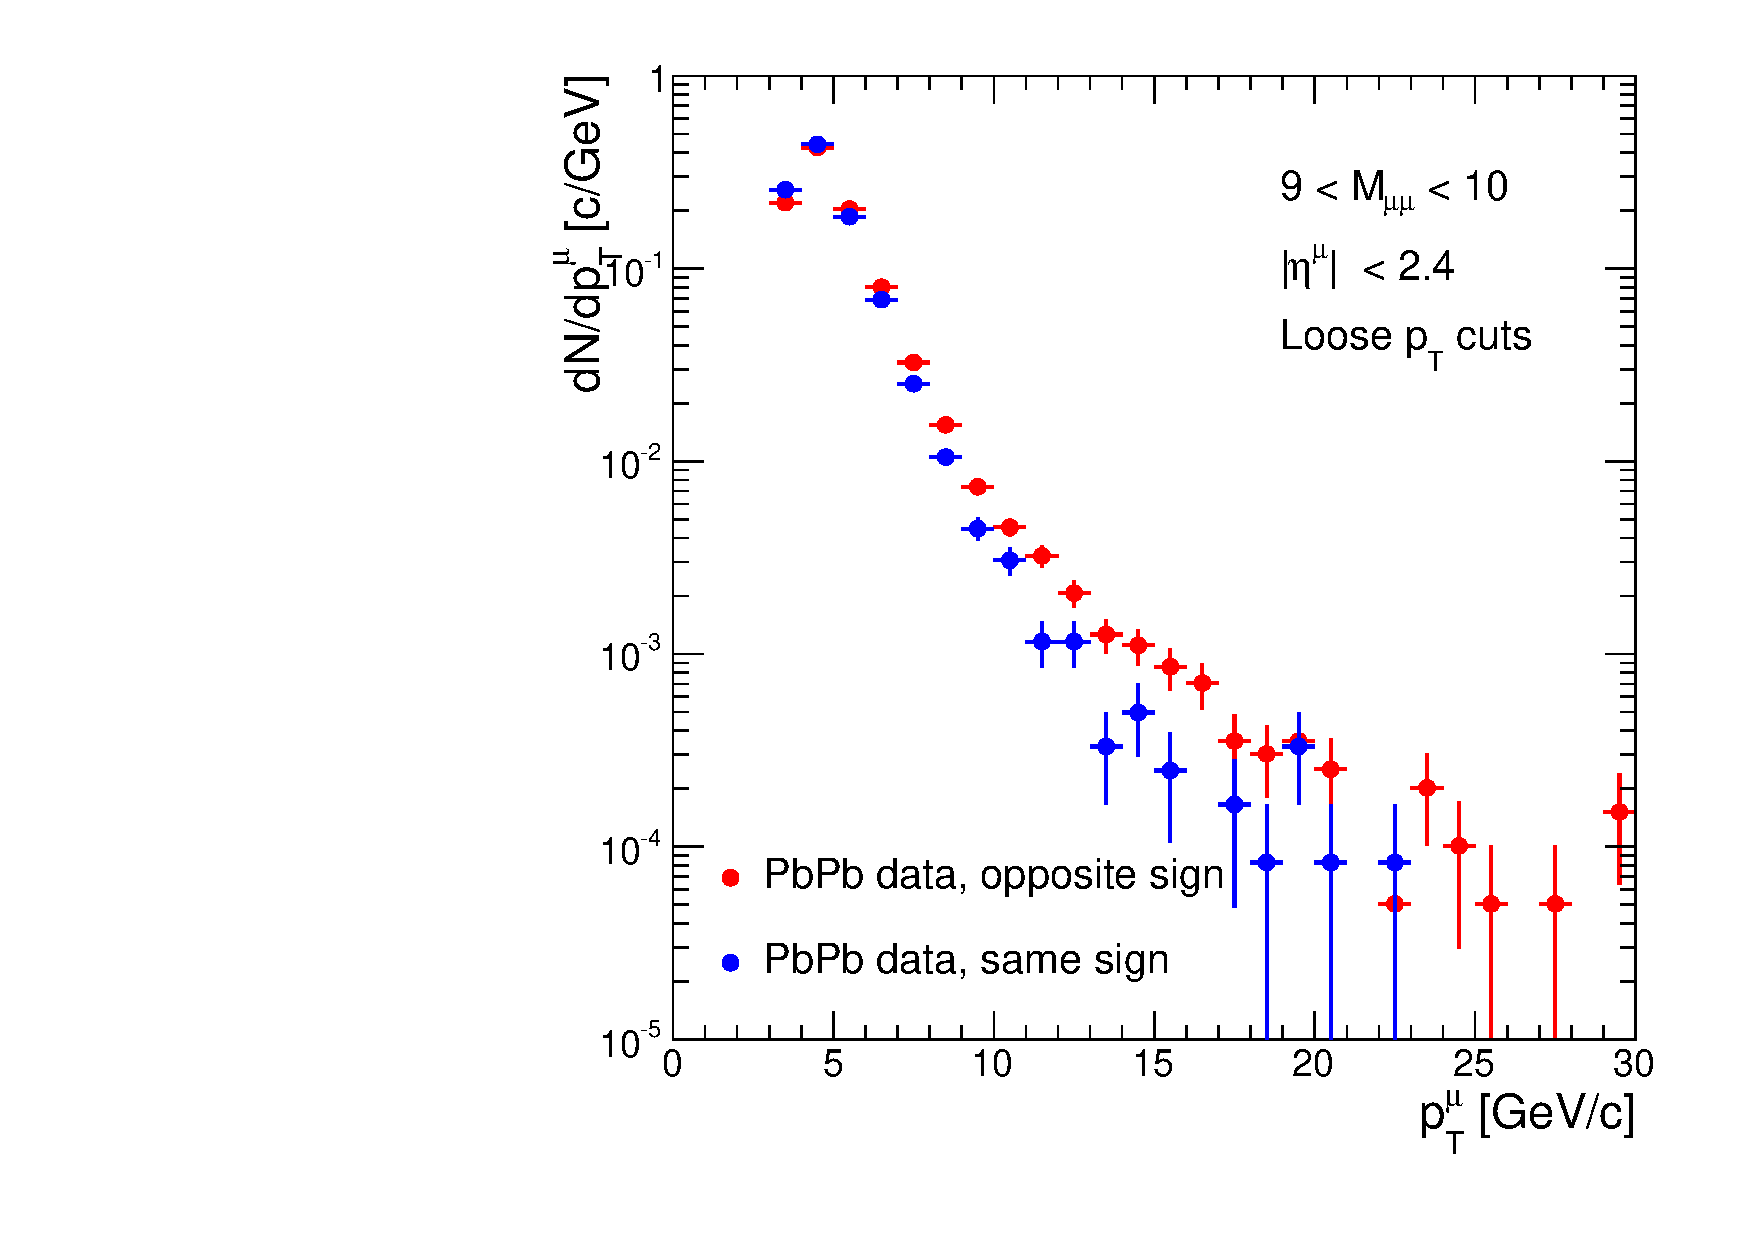
\includegraphics[width=0.49\textwidth]{Chapters/aCorrection/pt_aa_samesign.pdf}
%  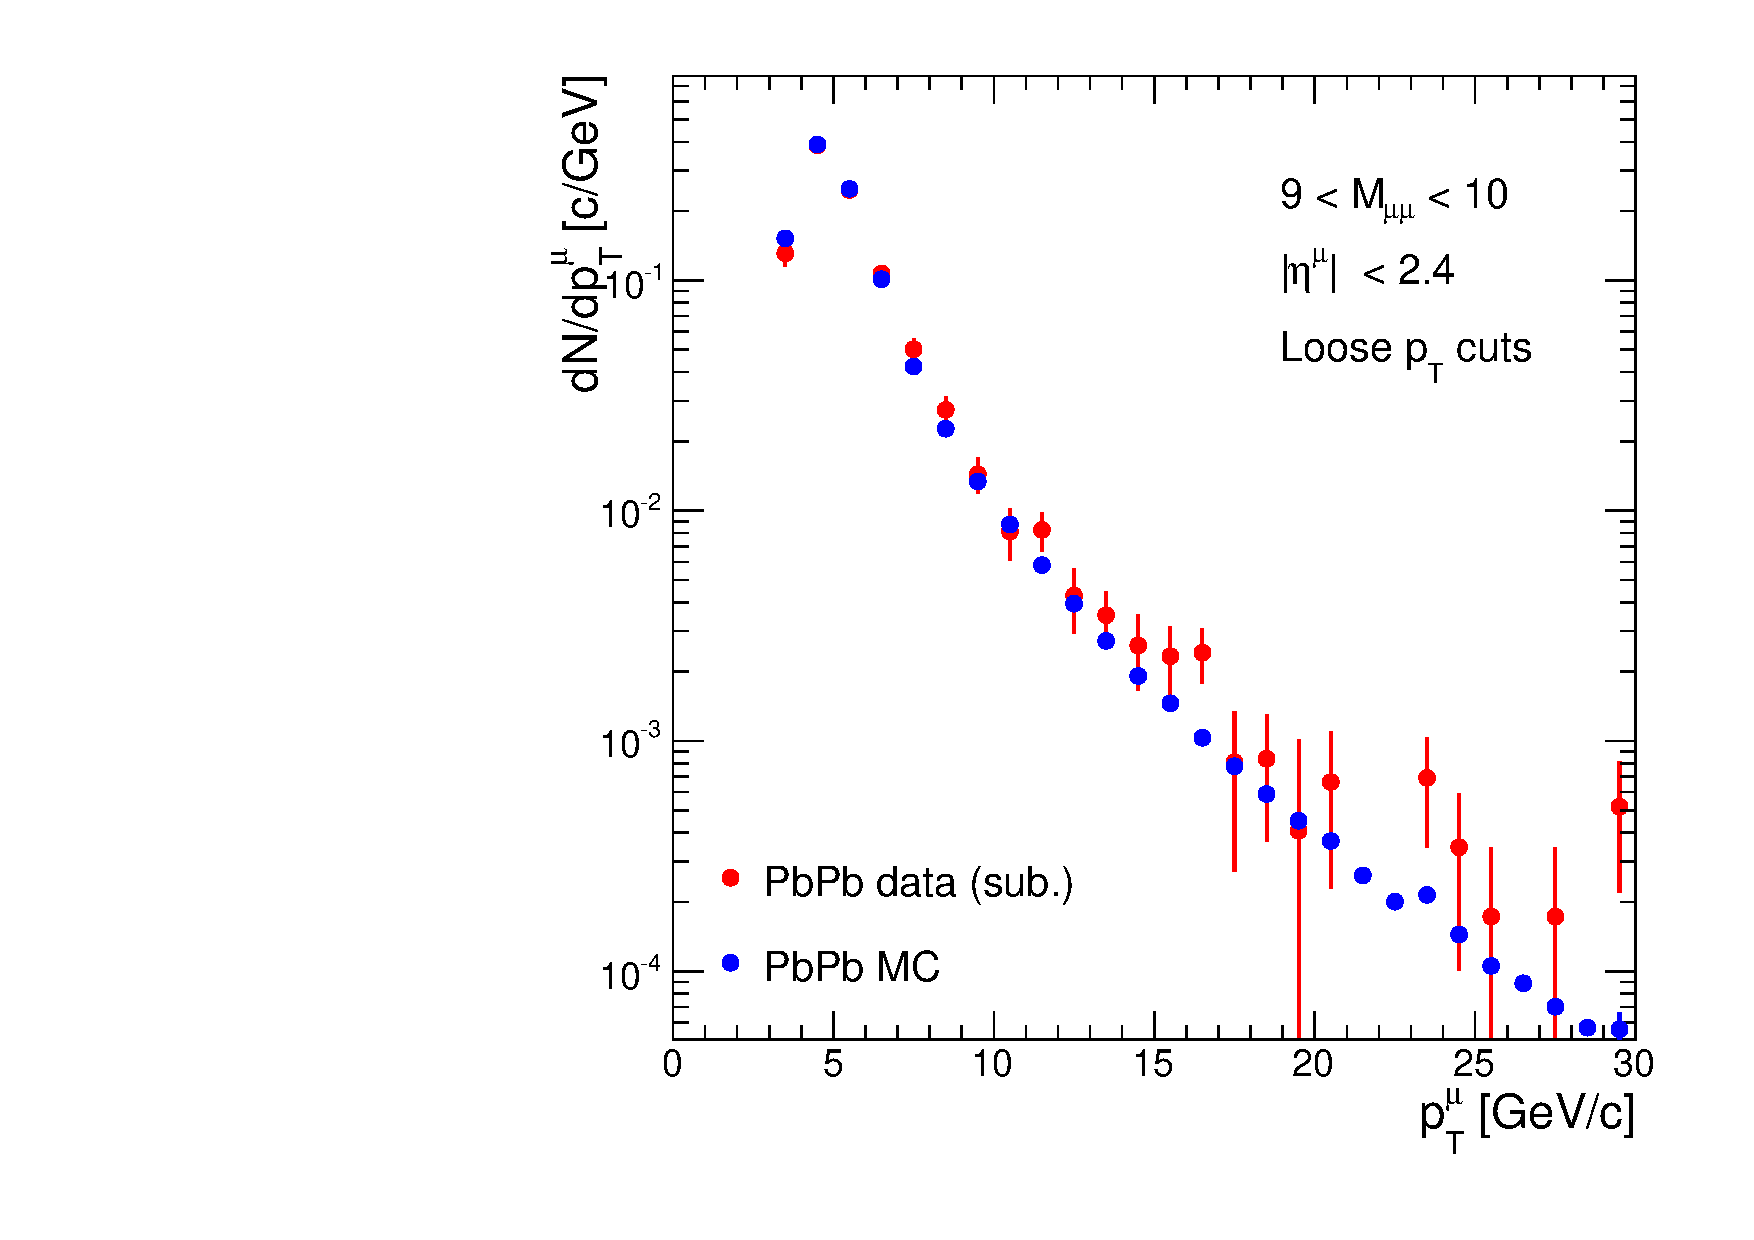
\includegraphics[width=0.49\textwidth]{Chapters/aCorrection/pt_aasub_MC.pdf}
%  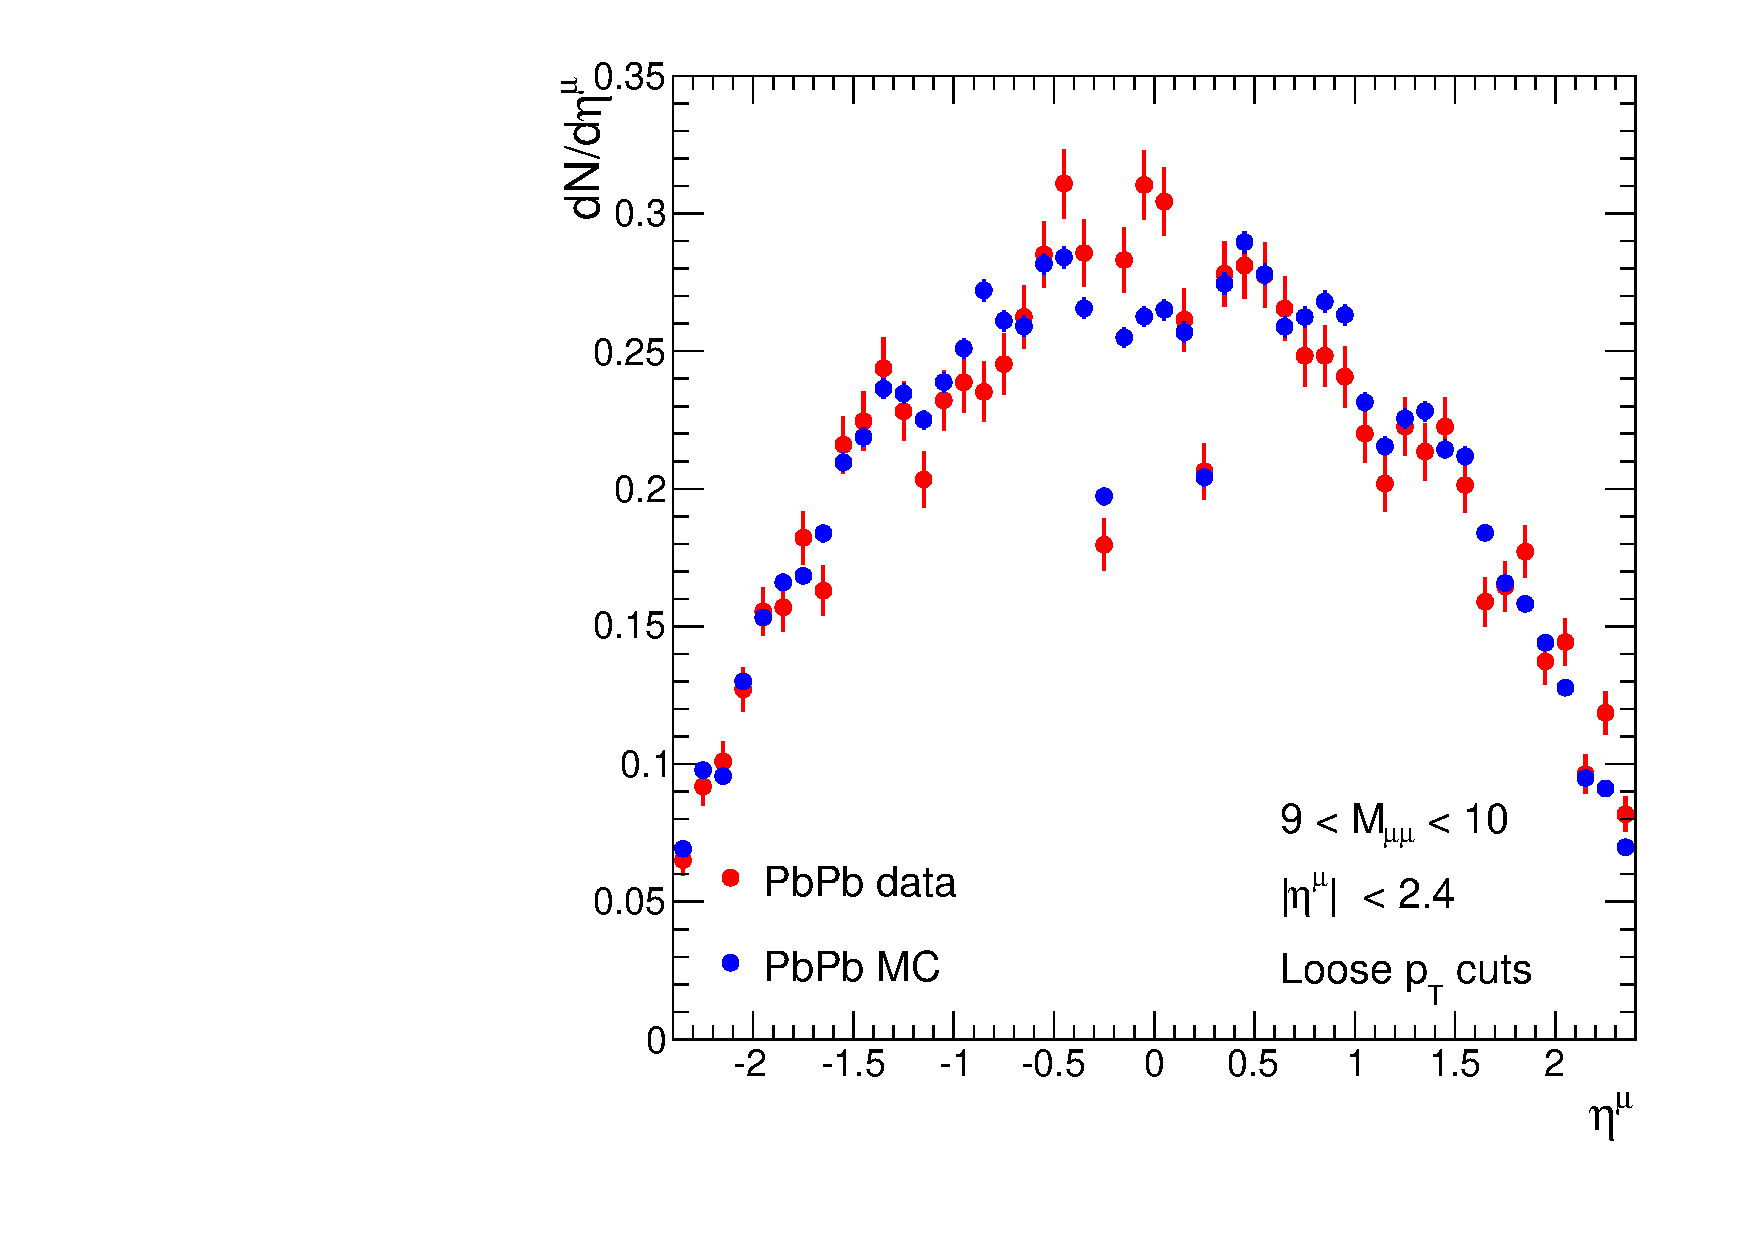
\includegraphics[width=0.49\textwidth]{Chapters/aCorrection/eta_aa_MC.pdf}
  \caption{Single muon \pt\ distributions. Muons come from dimuon
    pairs in the mass region of the \PgU, $9 < M < 10$~\unitMass. In
    both panels, red symbols represent the muon \pt\ distribution in
    PbPb collisions. On the left panel, muons from generated \PgU\ are in
    blue. On the right, muons from same-charge pairs are in blue.
  }
  \label{fig:pt_mcdata}
\end{centering}  
\end{figure}

One can point out that the $\pt$ distribution is harder in the Monte Carlo
than in the data. In order to investigate the origin of this
discrepancy, we first compare the distributions of same charge muons
(hence, background only) and opposite charge muons (with signal and
background contributions). We find that the $\pt^\mu$ distribution of
same charge muons is softer than that of opposite charge muons, as can
be seen in Figure~\ref{fig:pt_mcdata} (right). This could indicate that
the background yields softer $\pt^\mu$ distributions, thus possibly
explaining the discrepancy observed on the opposite charge muon
$\pt^\mu$ distributions in the data (hence, signal and background) and
in the Monte Carlo (only signal generated). 

\begin{figure}[h]
\begin{centering}  
 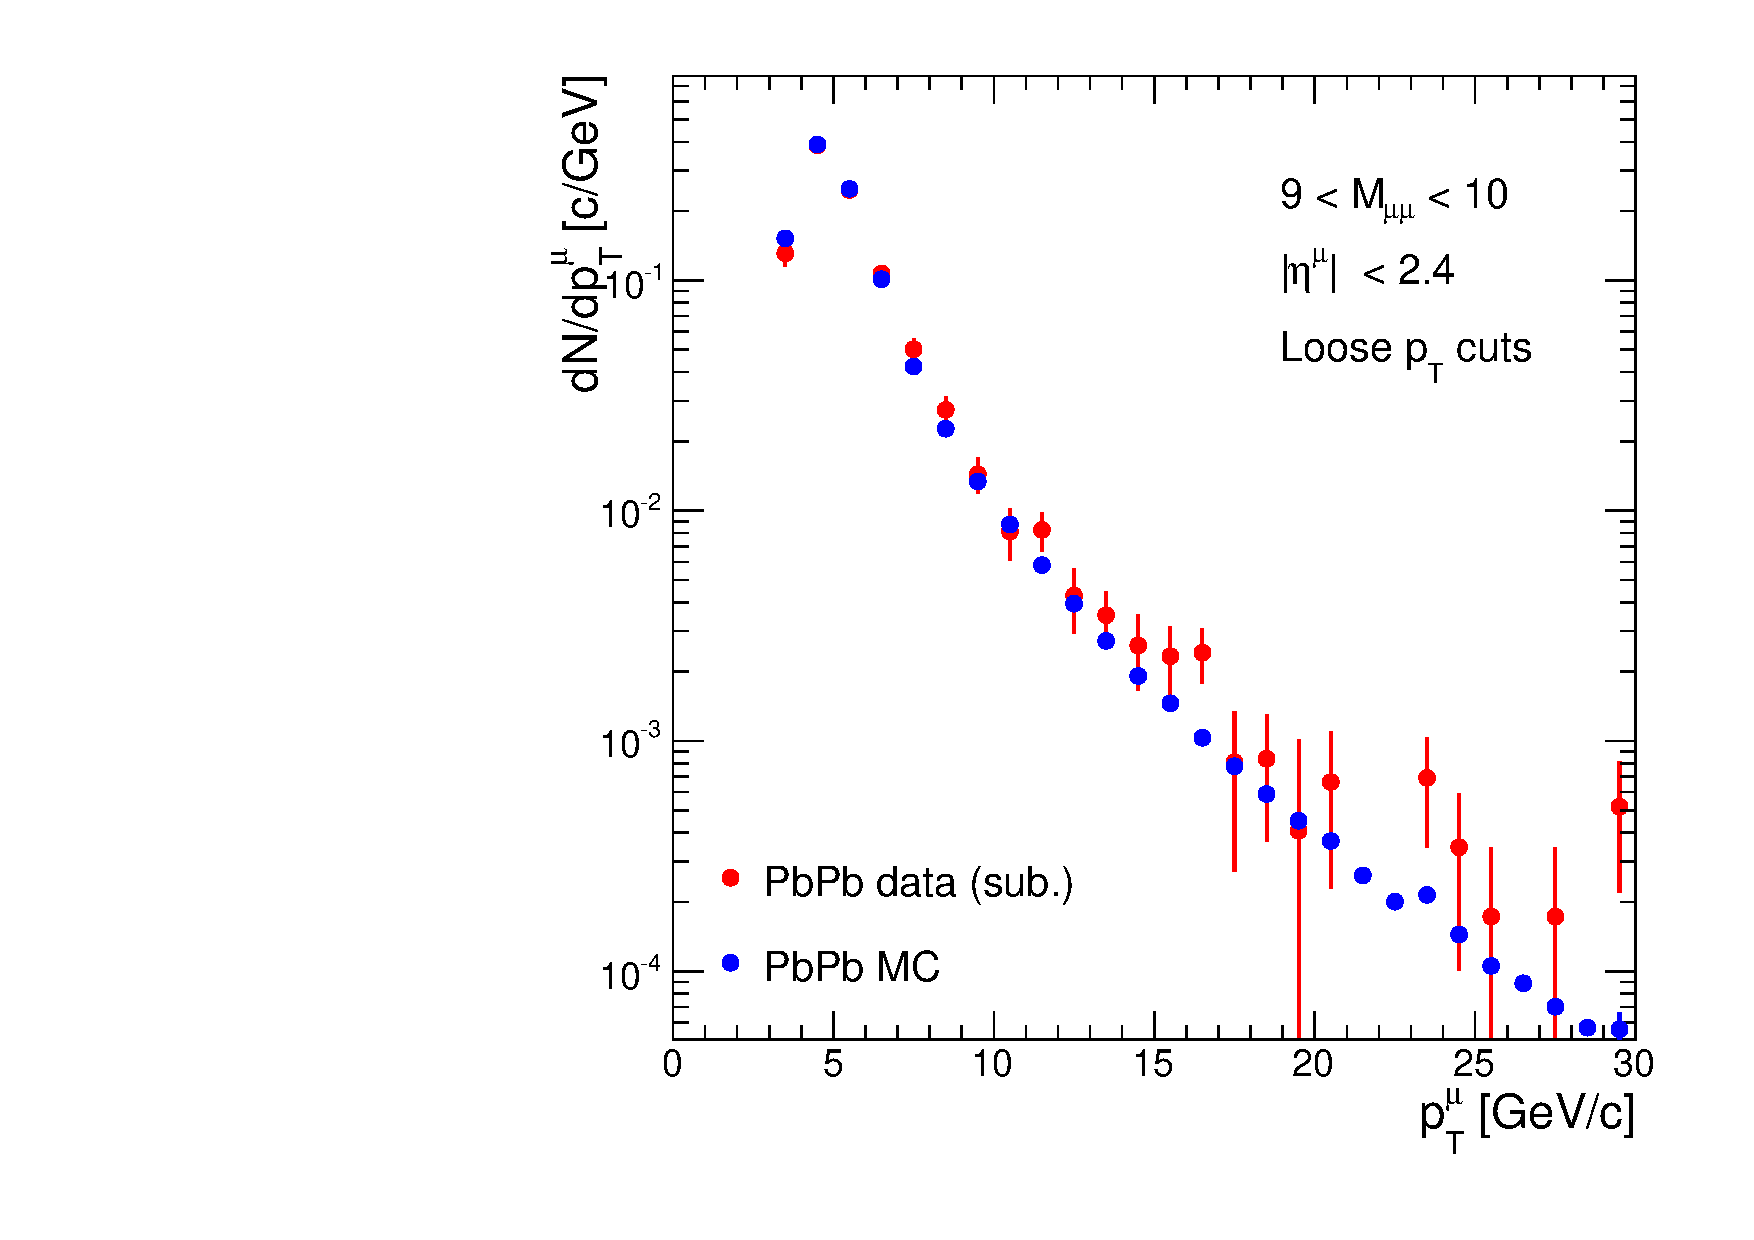
\includegraphics[width=0.5\textwidth]{Chapters/aCorrection/pt_aasub_MC.pdf}
  \caption{\pt\ distribution of single muons from pairs in the mass
    region of the \PgU. Right: background subtracted data is
    in red, and muons from generated \PgU\ are in blue.
  }
  \label{fig:datasubMC}
\end{centering}  
\end{figure}



For the sake of this comparison, we have therefore \emph{corrected} the data by performing a background subtraction to the opposite-charge $\pt^\mu$ distributions to check whether the actual discrepancy between PbPb data and Monte Carlo is due to the background contribution and not from a genuine MC failure. Assuming that the $\pt^\mu$ distribution from the background has the same shape as that from the same-charge sample, the 'background-subtracted' data reads
 \begin{equation}
\frac{dN^{\rm sub}}{d\pt} = \frac{dN^{\rm opp.\ charge}}{d\pt} - \frac{N^{\rm bkgd}}{N^{\rm same\ charge}}\ \frac{dN^{\rm same\ charge}}{d\pt},
 \end{equation}


where $N^{\rm same\ charge}$ and $N^{\rm bkgd}$ are respectively the number of same-charge events and the number of background events in the mass range $9<M<10$~GeV/$c^2$. Assuming that the number of (full) background events over the number of same-charge events is identical in the mass ranges $[8;9]$~\unitMass and $[9;10]$~\unitMass, we estimate the number of background events in the signal mass range to be given by $N^{\rm bkgd}=N^{\rm opp.\ charge}(8<M<9)/N^{\rm same\ charge}(8<M<9)*N^{\rm same\ charge}$. This corrected distribution is compared to the Monte Carlo prediction in Figure~\ref{fig:datasubMC} and now shows a very good agreement, giving confidence in the Monte Carlo used to compute acceptance and efficiency corrections.


\subsection{Data-MC comparisons of muon quality}
\label{sec:data_mc_muon}
% I will first summarise here the various quality cuts (already presented in
% Section~\ref{sec:muonID}).

 Understanding the effect of the muon identification cuts is
especially important for the estimation of the dimuon reconstruction
efficiency. As we have seen in Section~\ref{sec:eff}, the
reconstruction efficiency can be split in three main parts:

\begin{equation}
\eff = \eff(\rm trig) \cdot \eff(\rm ID) \cdot \eff(\rm trk)
\end{equation}

where \eff(trig) is the trigger efficiency, \eff(ID) is
the result of applying identification cuts, and \eff(trk) is
the silicon tracker's tracking efficiency. Note that I have not
specified whether I speak about muons or \PgU\ or any other
particle. This point will be assessed later. The identification efficiency
for muons, \eff(MuonID), is defined to estimate the effect of the
following cuts:

\begin{itemize}
    \item[-] each muon-track has been measured in at least one pixel
      layer, 
    \item[-] number of tracker hits of the muon-track $>$ 10, 
    \item[-] reduced $\chi^{2}$ of the muon-track $<$ 4,
    \item[-] reduced $\chi^{2}$ of the global muon $<$ 10, 
    \item[-] transverse impact parameter of each muon with respect to the primary
      vertex, D$_{\textrm{xy}}$ $<$ 3 cm,
    \item[-] longitudinal impact parameter of each muon with respect to
      the primary vertex  D$_{\textrm{z}}$ $<$ 15 cm,
    \item[-] The track is arbitrated: coincides with an existing STA muon within 3
      times the spread of the muon track in the x-y plane.
    \item[-] isGlobalMuon() and isTrackerMuon()
      (cf. Section~\ref{sec:muonID} for more information).
\end{itemize}

The plots in Figure~\ref{fig:muonIDplots} show a study of the Data and MC
distributions for events in the \Jpsi mass range (used for the much
larger statistics than in the \PgU\ case), passing the above
cuts only. i.e. no \pt(\Pgm) or trigger requirement was applied. The detail of
each distribution is quite clear: there are a few discrepancies,
and it is believed that these discrepancies may result in a mis-conceived
MC dimuon efficiency.

\begin{figure}
  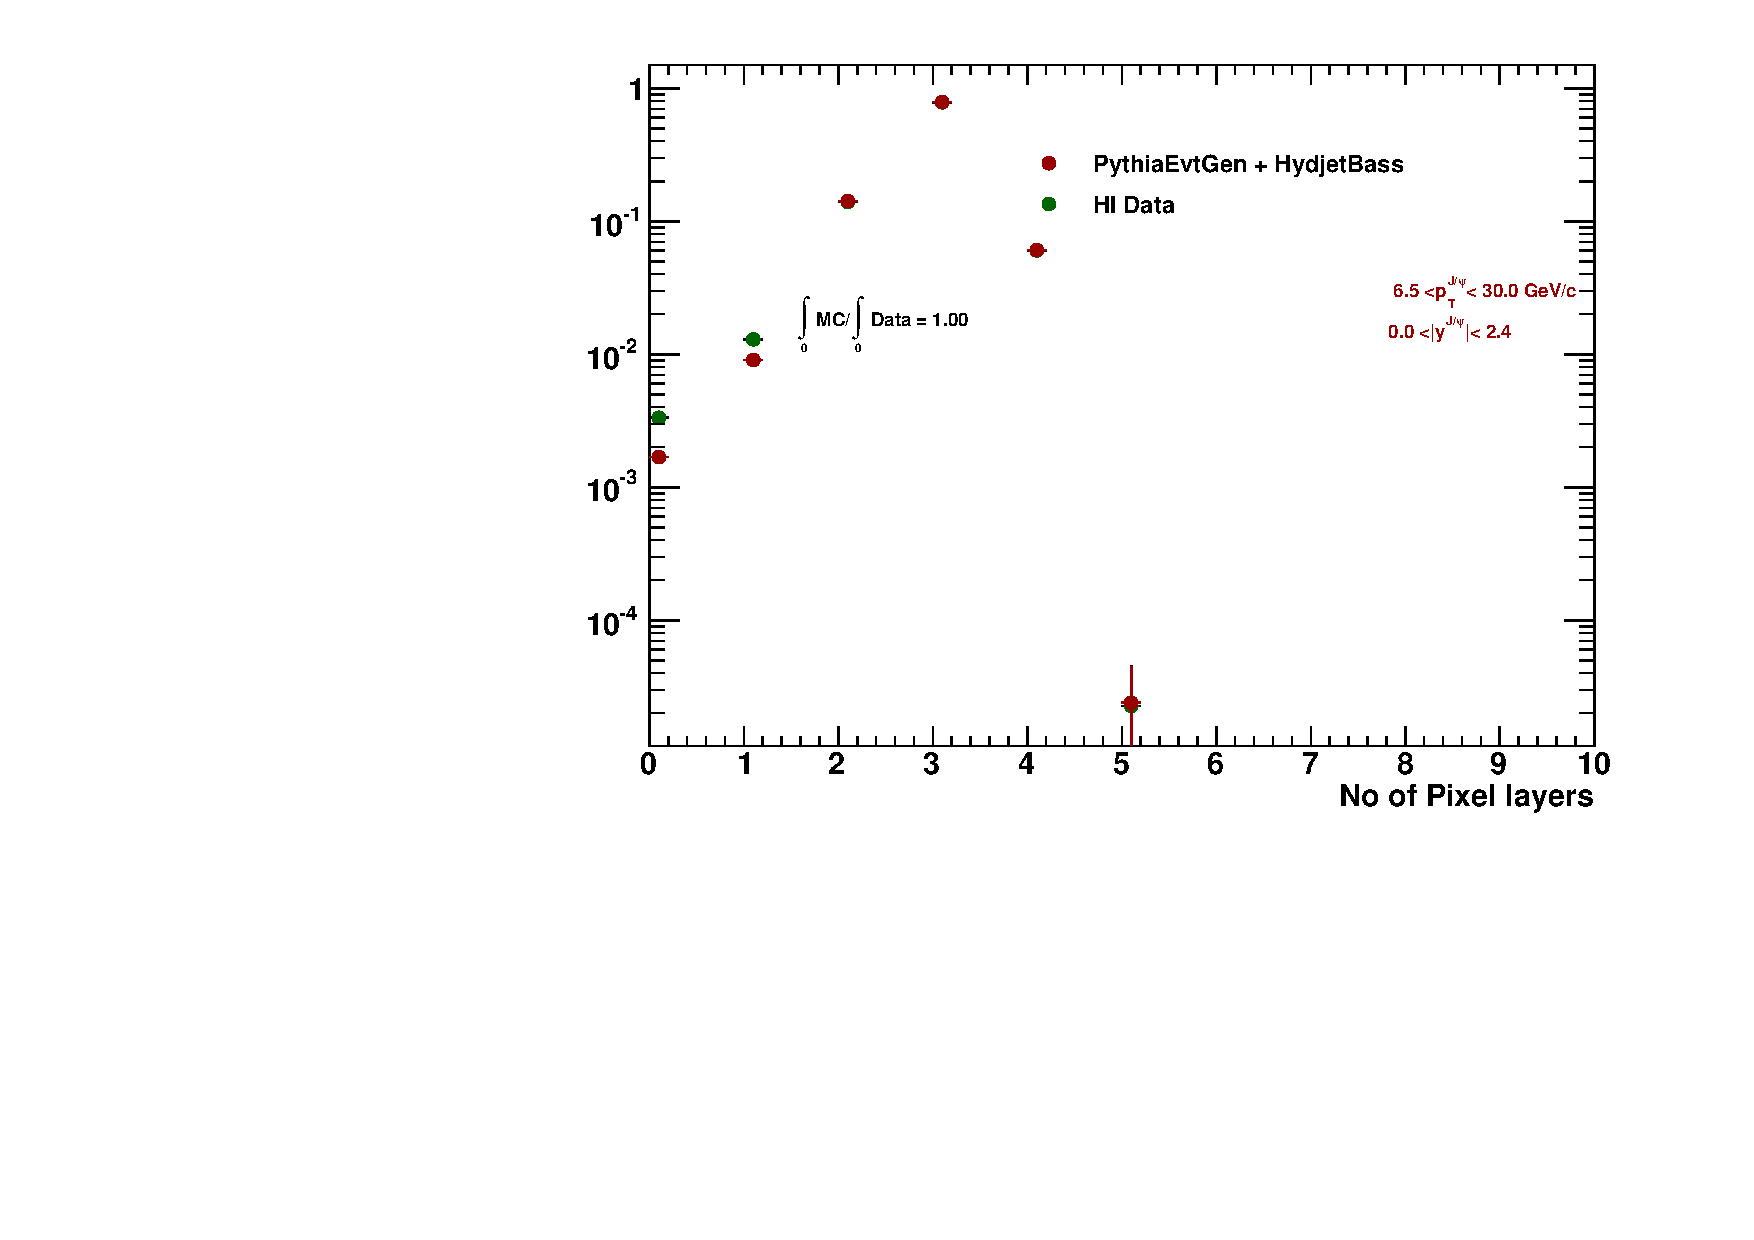
\includegraphics[width=0.32\textwidth]{Chapters/aCorrection/PixelLayer.pdf}
  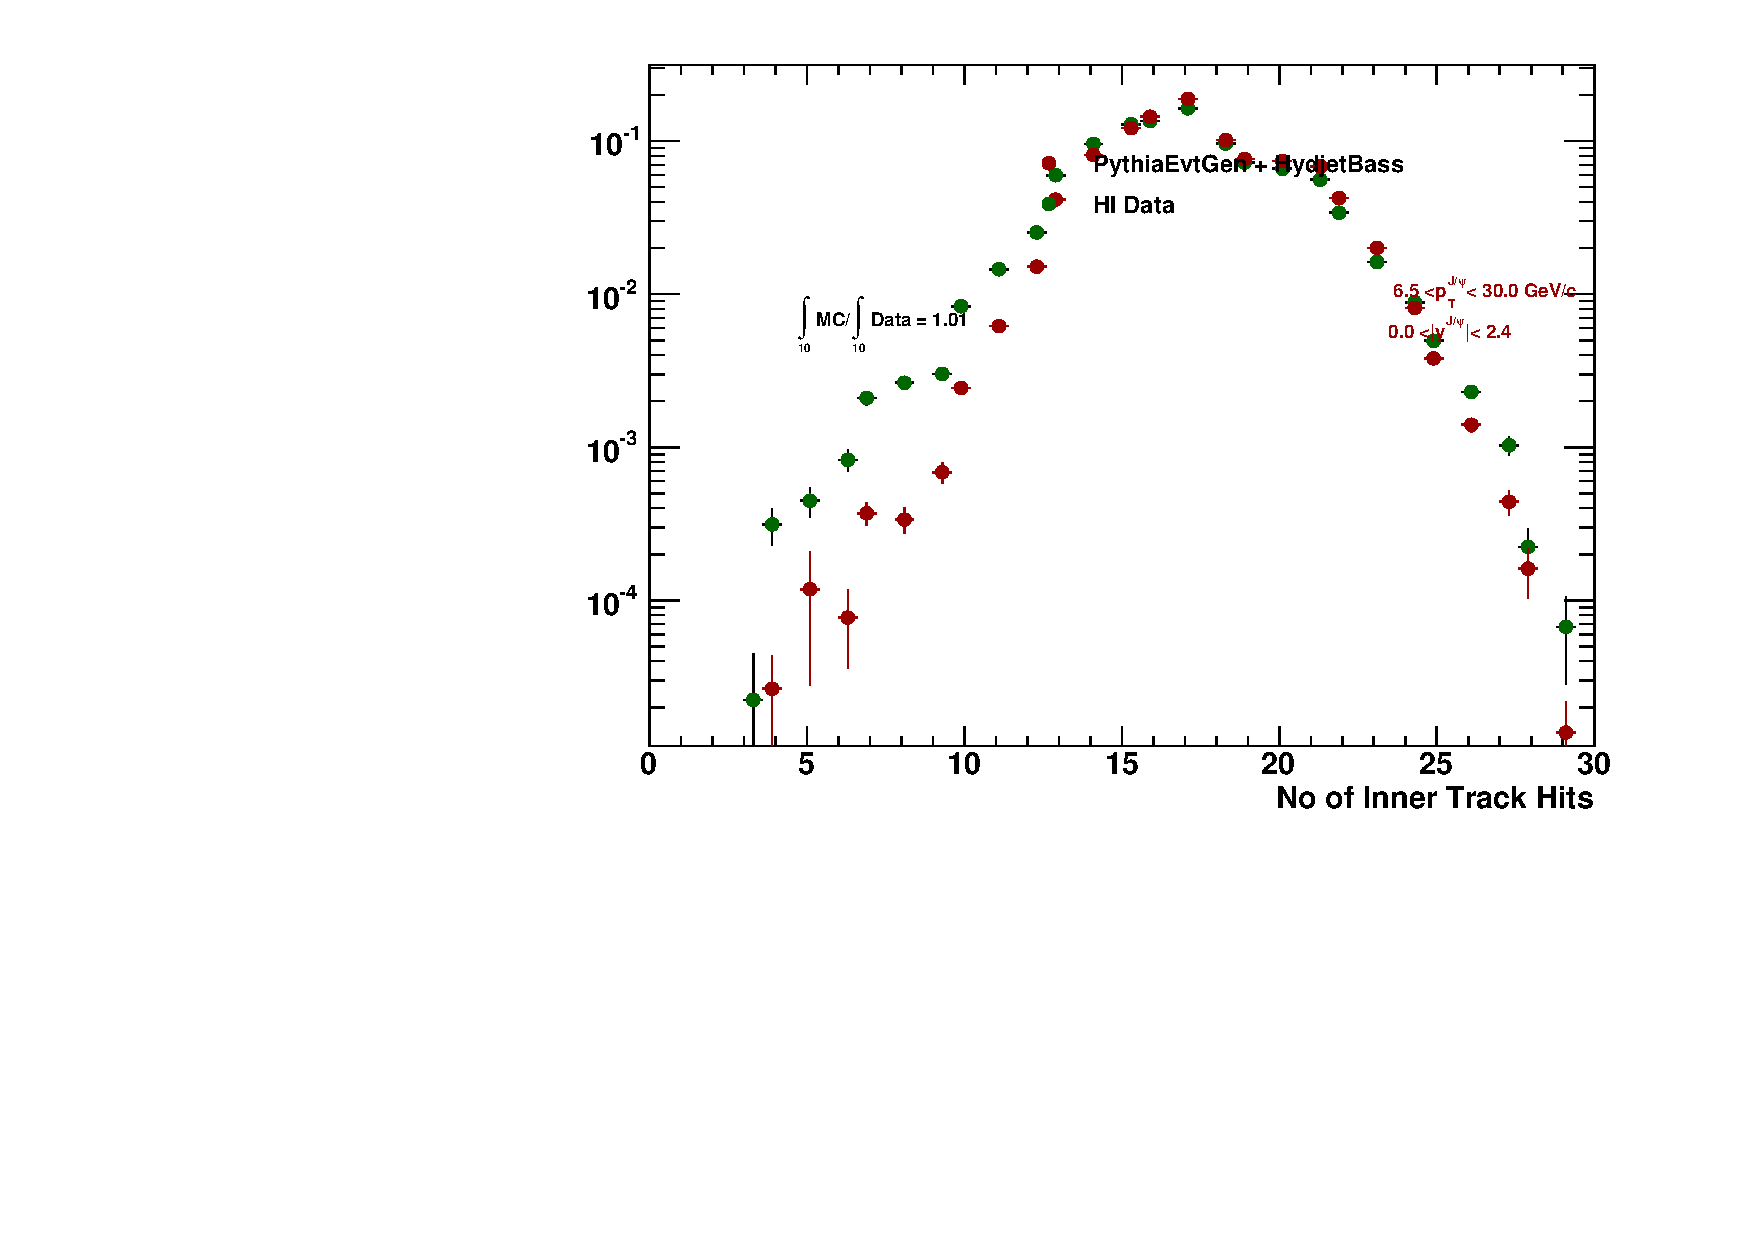
\includegraphics[width=0.32\textwidth]{Chapters/aCorrection/InnerTrackHits.pdf}
  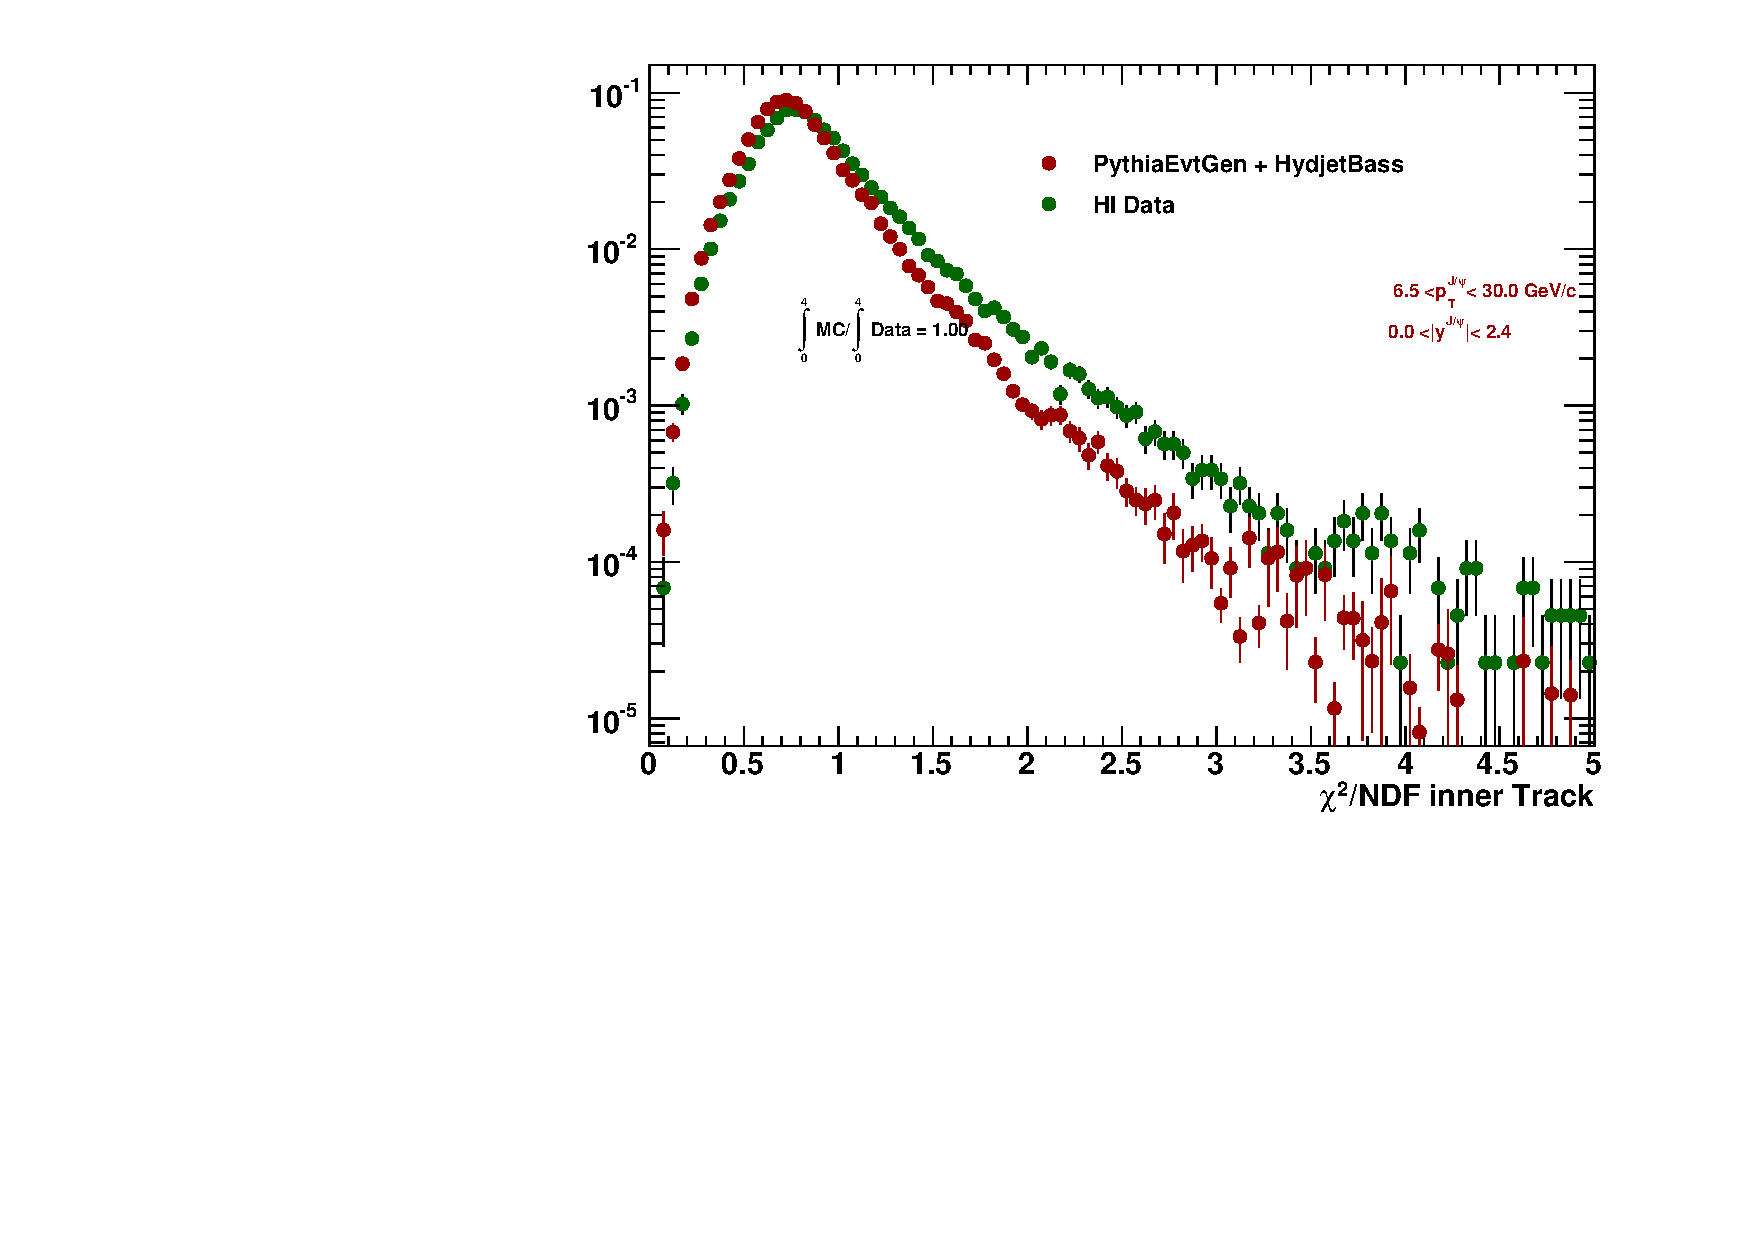
\includegraphics[width=0.32\textwidth]{Chapters/aCorrection/Chi2NdfInner.pdf}
  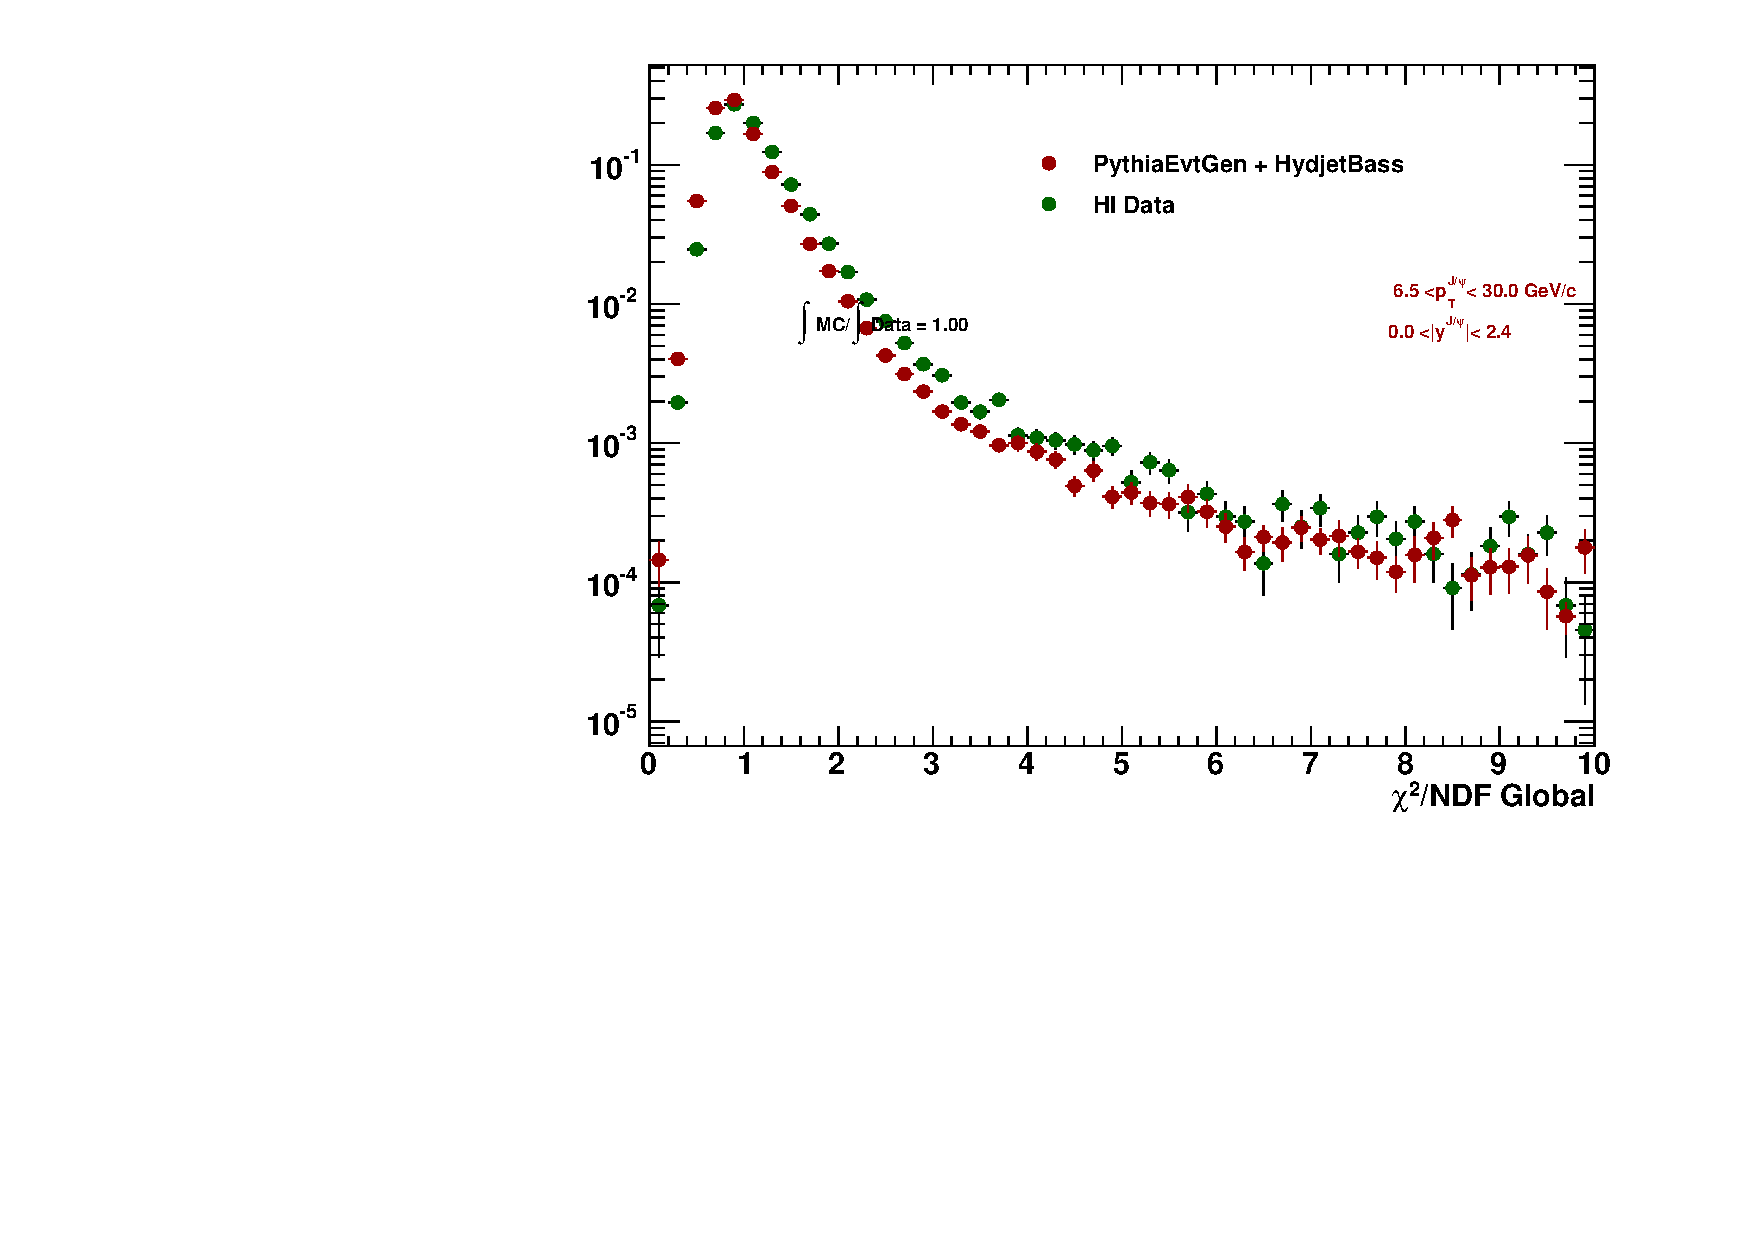
\includegraphics[width=0.32\textwidth]{Chapters/aCorrection/Chi2NdfGlobal.pdf}
  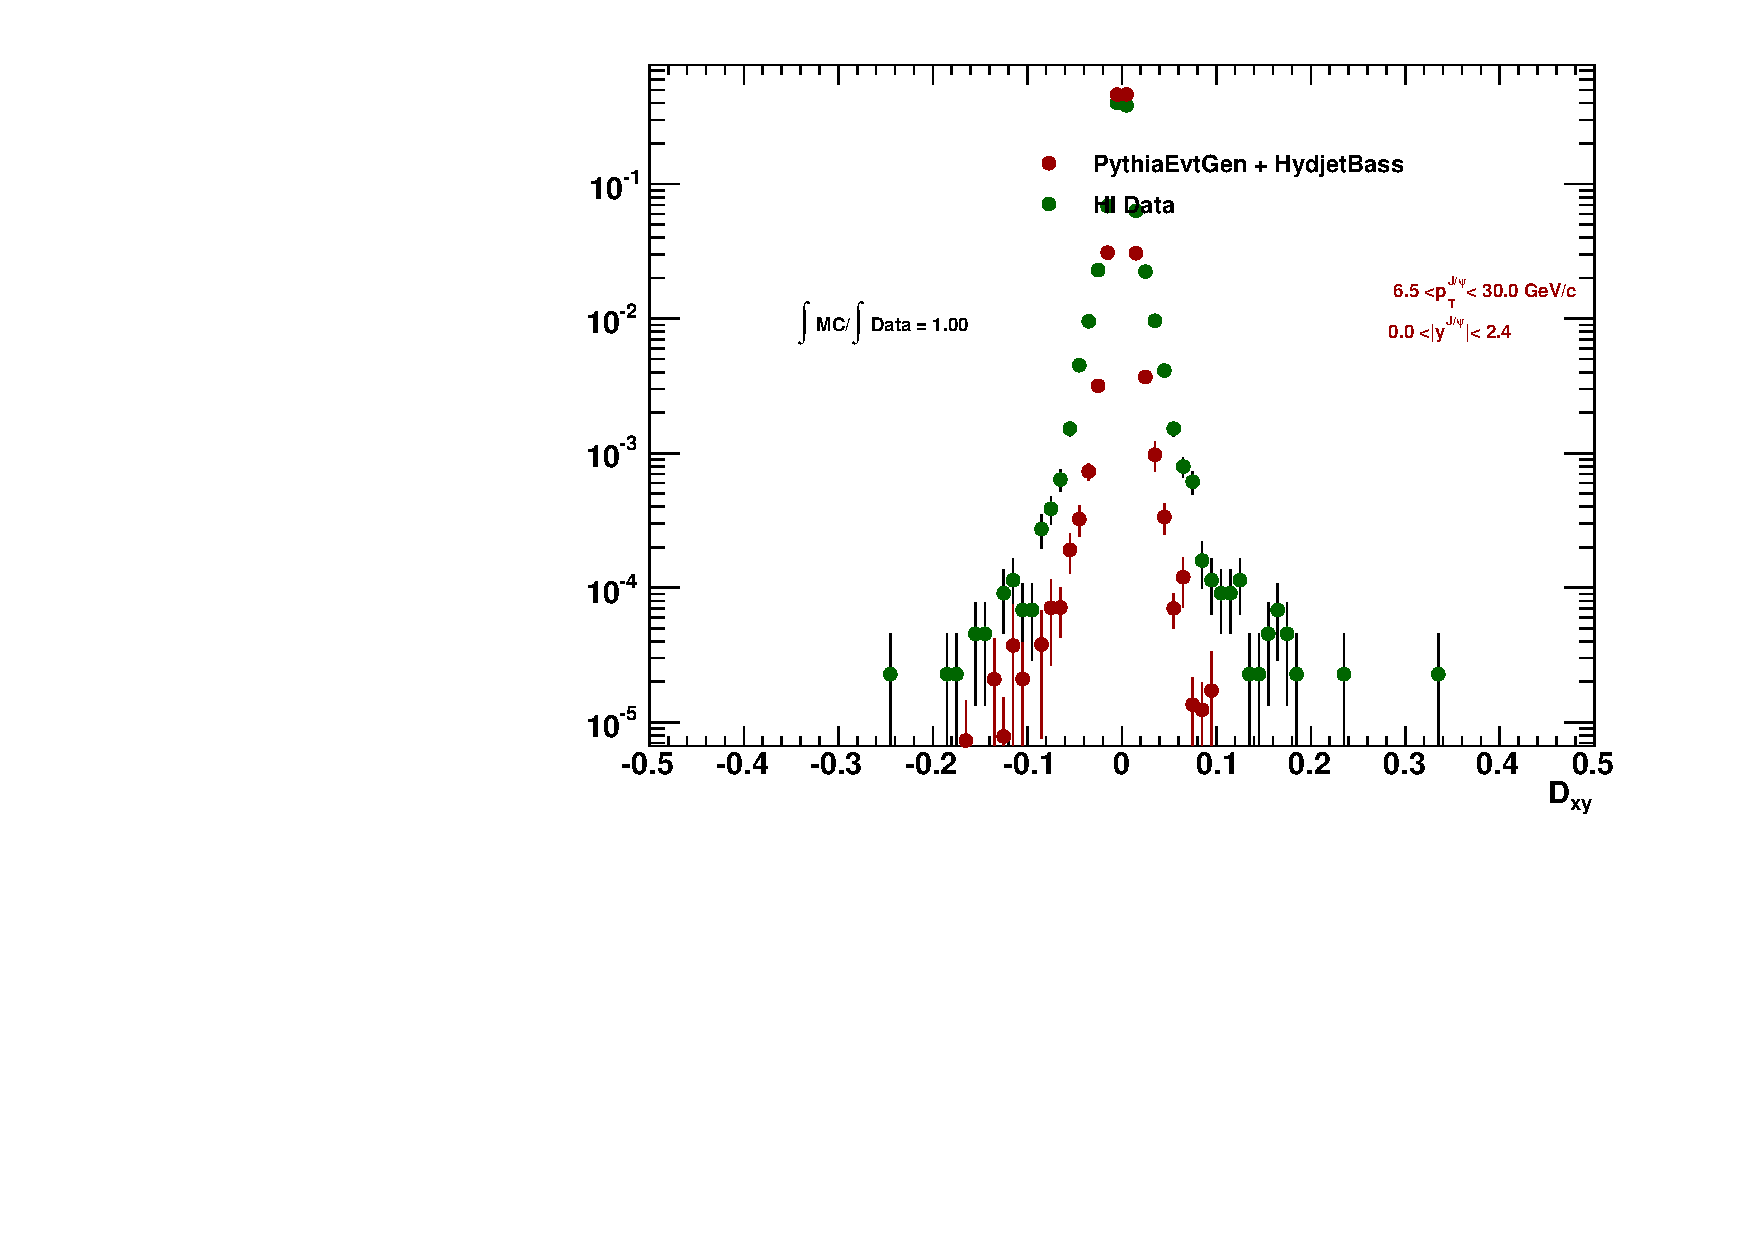
\includegraphics[width=0.32\textwidth]{Chapters/aCorrection/Dxy.pdf}
  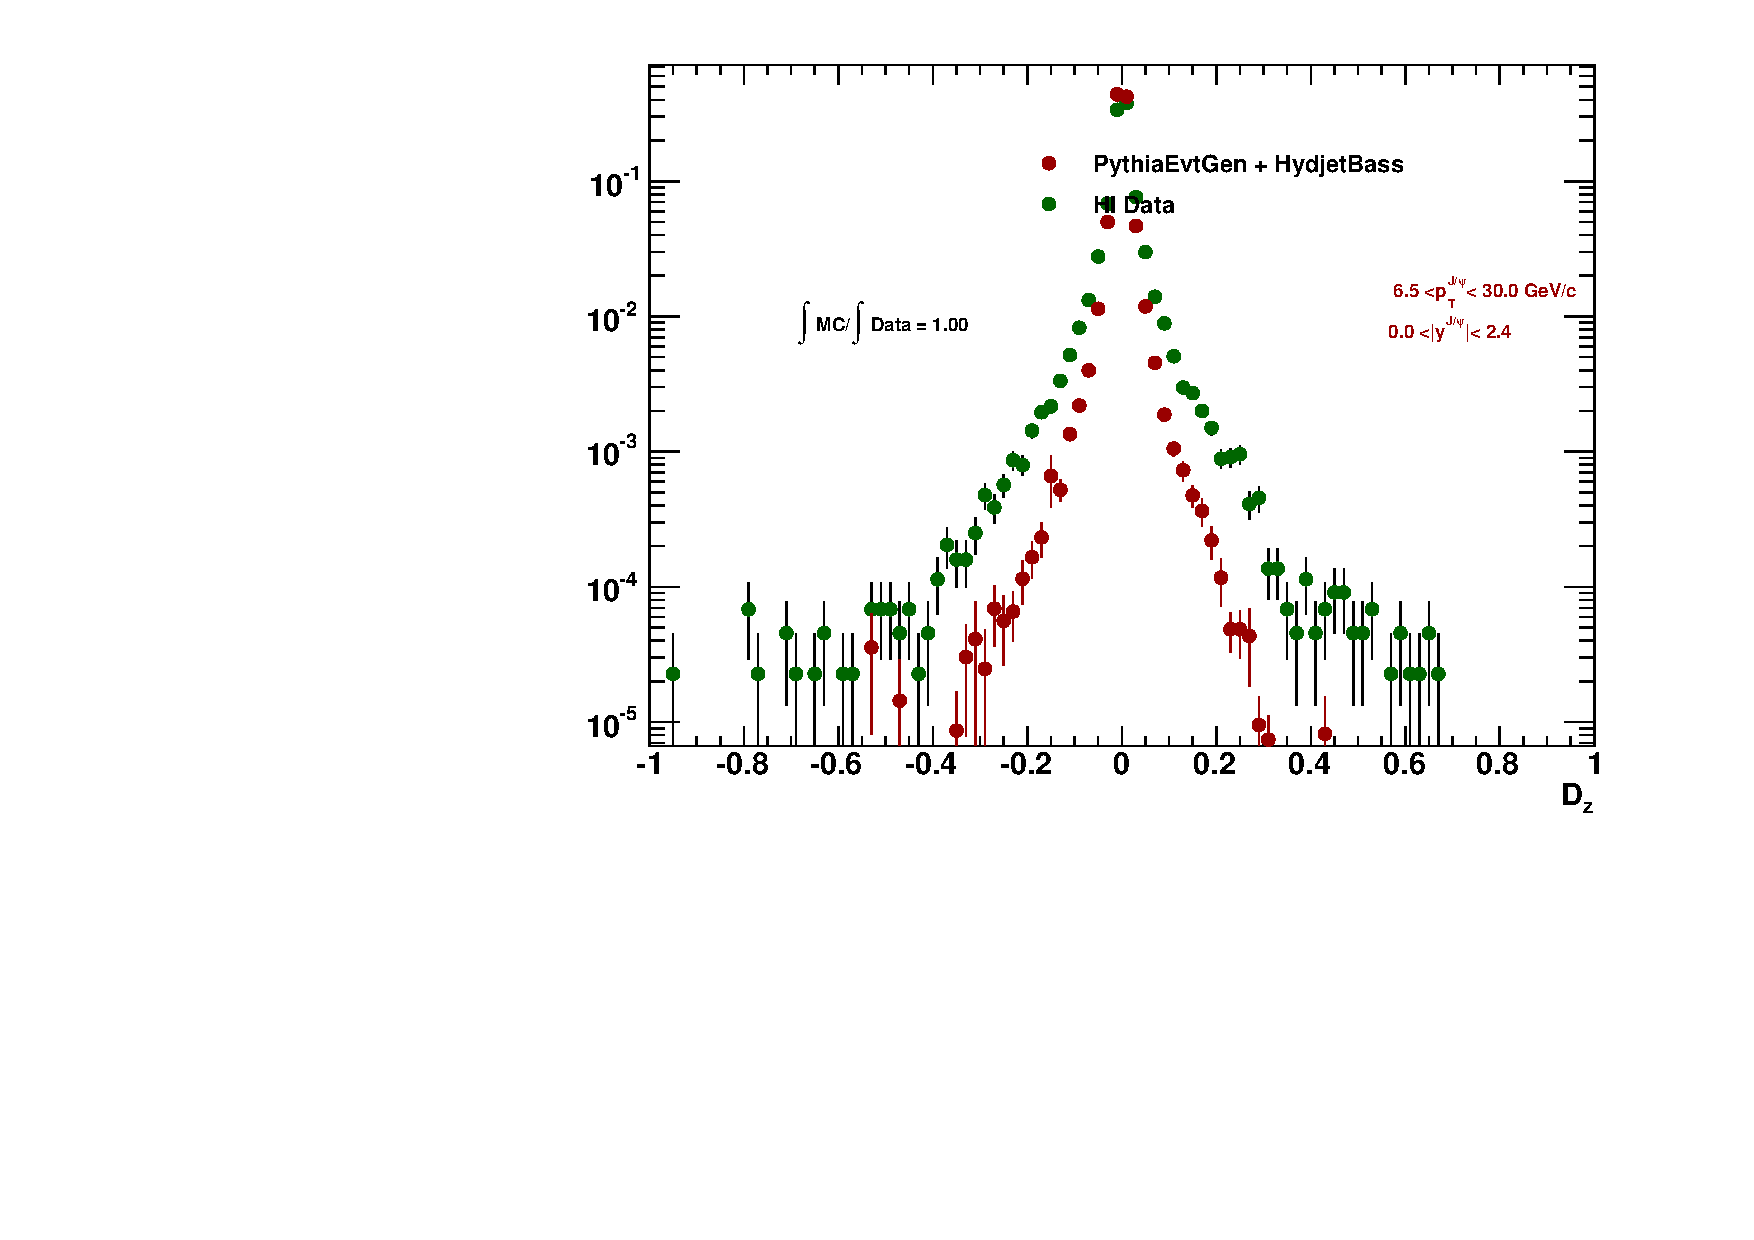
\includegraphics[width=0.32\textwidth]{Chapters/aCorrection/Dz.pdf}
%  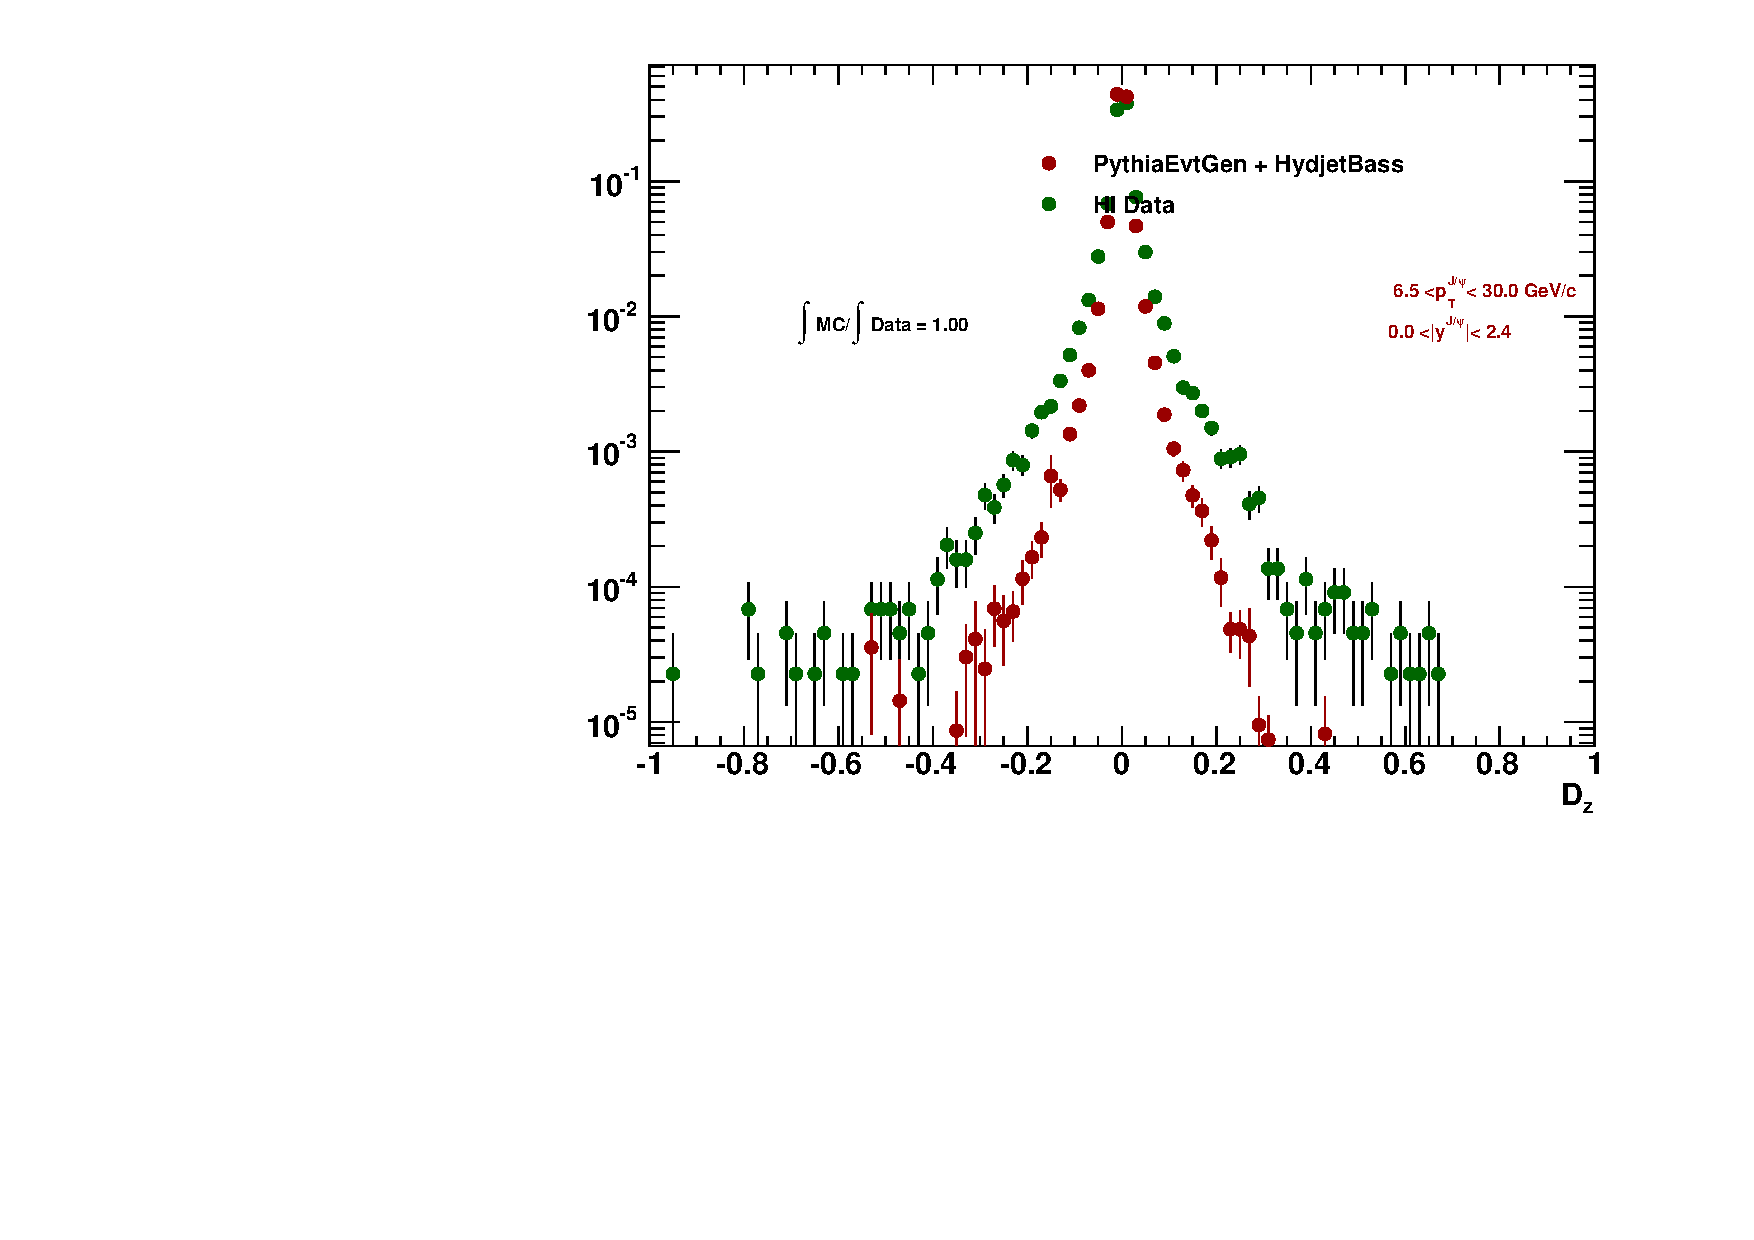
\includegraphics[width=0.3\textwidth]{Chapters/aCorrection/Dz.pdf}
 \caption{Tracker muon and global muon quality variables in MC and
   Data. Muons used are \Jpsi decay muons.}
 \label{fig:muonIDplots} 
\end{figure}

\subsection{The Tag and Probe method}
\label{sec:tnp}
In data analysis, one of the most important elements is to estimate the efficiency
accurately and reliably. Monte Carlo (MC) simulation is generally used for the estimation
of the efficiency but produces large systematic uncertainties due to the imperfections
in modeling the detector response. Therefore, any measure of the
particle efficiency from the data itself is of tremendous interest.
One well established data-driven approach to measure efficiencies of particles is
the `Tag and Probe' technique~\cite{1748-0221-7-10-P10002}.


The Tag and Probe method utilizes a known mass resonance (e.g. \Jpsi,
\PgU, Z) to select decay particles, and probe the efficiency of a particular selection criterion on those particles. In general the "tag" is an object
that passes a set of tight selection criteria designed to isolate the required particle type (usually an electron or muon,
though in principle the method is not strictly limited to these). Tags are often referred to as "golden" electrons or muons,
and the fake rate for passing tags selection criteria should be very small. A generic set of the
desired particle type (i.e. with potentially very loose selection criteria) known as "probes" is selected by paring
these objects with tags such that the invariant mass of the combination is consistent with the mass of the resonance.
Combinatorial backgrounds may be eliminated through any of a variety of background subtraction methods
such as fitting, or sideband subtraction. The definition of the probe object depends on the specifics of the
selection criterion being examined.

Invariant mass plots are then made by requiring (or not) the probed
criterion to be passed. The ratio of the number of resonances obtained
with (or without) the probed criterion, measures its efficiency.

Since 2010, this method has been employed in CMS, in particular in the
heavy ion group, for the validation of efficiencies measured with MC,
as in~\cite{torsten, HIN-11-007, HIZpaper, HIPsiPaper}.
The data-driven Tag and Probe method will be employed to estimate single-muon trigger, identification,
and tracking efficiencies. A comparison of the results obtained by applying the technique
to both data and MC simulation allows to estimate related systematic uncertainties.
The \Jpsi signal resonance is used for its large rate of production.
Two tag-probe invariant mass distributions are formed, in the vicinity of the \Jpsi nominal mass,
according to whether the probe passes or fails the criteria for which
the efficiency is being measured. 


Depending on the (\pt, \Pgh) bin considered, the passing and failing
probes peak can be more or less difficult to fit. In the following
Figure~\ref{fig:pp_tnp_fits_example}, I have chosen an example where
the pp tracking efficiency is taken from MC tag-probe pairs on the
left and from real data on the right. In the following, I will detail more the various parts of
the Tag and Probe workflow.

\begin{figure}
  \begin{center}
    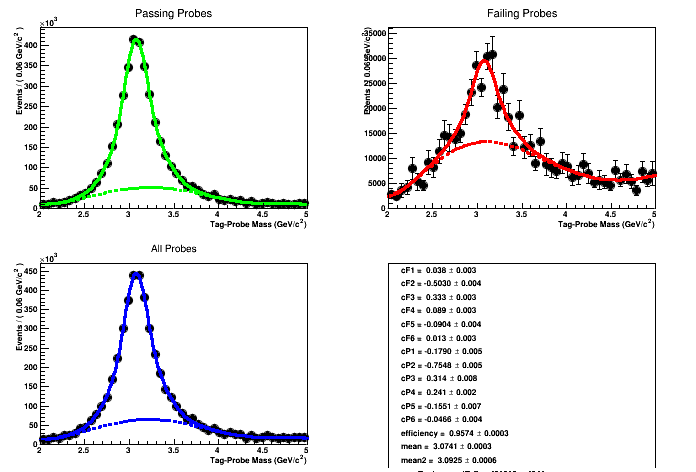
\includegraphics[width=0.45\textwidth]{Chapters/aCorrection/mass_MC_trk.png}
    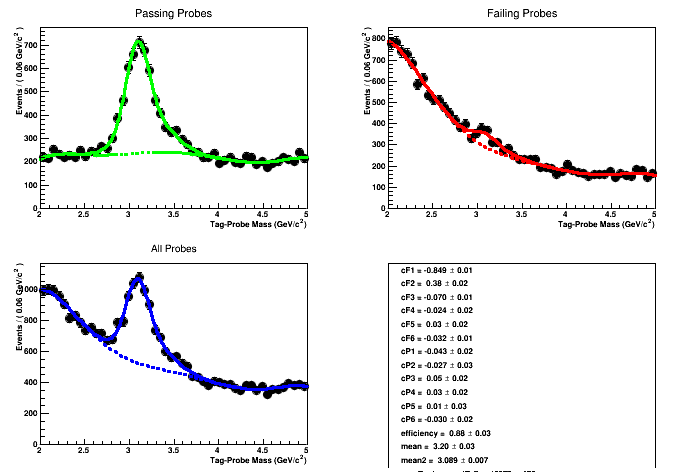
\includegraphics[width=0.45\textwidth]{Chapters/aCorrection/mass_RD_trk.png}\\
    \caption{Examples of $pp \to \Jpsi \to \mu\mu$ tag-probe invariant mass fits in data \emph{(right)}
     MC \emph{(left)}. Blue: tags paired to all probes, Red: tags
     paired to failing probes, Green: tags paired to passing
     probes. The ratio of (blue) and (green) integrated curves give
     the efficiency of the probed selection.
   }
    \label{fig:pp_tnp_fits_example}
  \end{center}
\end{figure}

% In heavy-ion dilepton analysis we do not use tag and probe measured efficiencies to
% correct the measured quarkonia yields due to several issues. One being
% the relatively small statistics sample of \Jpsi collected and the
% large background makes the measurement difficult. Furthermore,
% there are much more fundamental reasons, such as the remaining issues
% in measuring fake matching rates and/or the inner to outer track
% matching efficiency. One issue is that we cannot measure the fake
% efficiency in the way it was done in pp, as in heavy ions fake and
% tracking efficiency can be ``correlated'' due to the high
% multiplicity, i.e. one can have a fake match in events in which one has
% removed the true match. This problem was first encountered in the $Z$ boson
% analysis~\cite{HIZpaper}. Yet another problem is that measuring
% the matching efficiency ($\varepsilon_{\text{M}}$) between a
% standalone muon and an inner track (necessary to promote a standalone
% muon to a global muon) is not straight forward in heavy-ions.

\subsection{Single muon efficiencies}
\label{sec:tnp_mueff}

%rephrase
Here are defined the 'tag', 'probe' and 'passing probe' definitions used for
the combined efficiency of muon identification and trigger
requirements.%   discussed (cf. Section~\ref{subsec:def_trigID}), and muon
% tracking efficiencies (cf. Section~\ref{subsec:def_tracking})

The
tag muon selection/definition is the same in both cases: a
high-quality muon passing all analysis cuts, as described in the item
list above, that is matched to a single muon trigger. 
%The separate tag-and-probe results in the style of the preliminary results, are in \ref{sec:app_tagprobe}.

\subsubsection*{Trigger+ID efficiency}
\label{subsec:def_trigID}
\begin{itemize}
\item Muon reconstruction and identification efficiency (including the
  inner to outer track matching efficiency), and trigger efficiency within the single muon acceptance cut defined in Section~\ref{sec:sigext_fits}:
  \begin{itemize}
  \item probe: tracker muon in the acceptance, that pass inner tracker quality cuts
   \item passing probe: probe that is also a global muon passing all analysis selection cuts, and is matched to the HLT\_HIL1DoubleMu0\_HighQ (for PbPb) and HLT\_PAL1DoubleMu0\_HighQ (for pp).
   \end{itemize}
\end{itemize}
In the following Figure~\ref{fig:trigid_eff}, the resulting
single muon $pp$ and PbPb efficiencies from the tag and probe method are
presented in two phase space regions: First, the barrel (for
\pt(\Jpsi) above 6.5 \GeVc and muon $|\eta|$ <1.6) and second,
the forward (for \pt(\Jpsi) above 3 \GeVc and muon 1.6<$|\eta|$<2.4).

\begin{figure}
  \begin{center}
    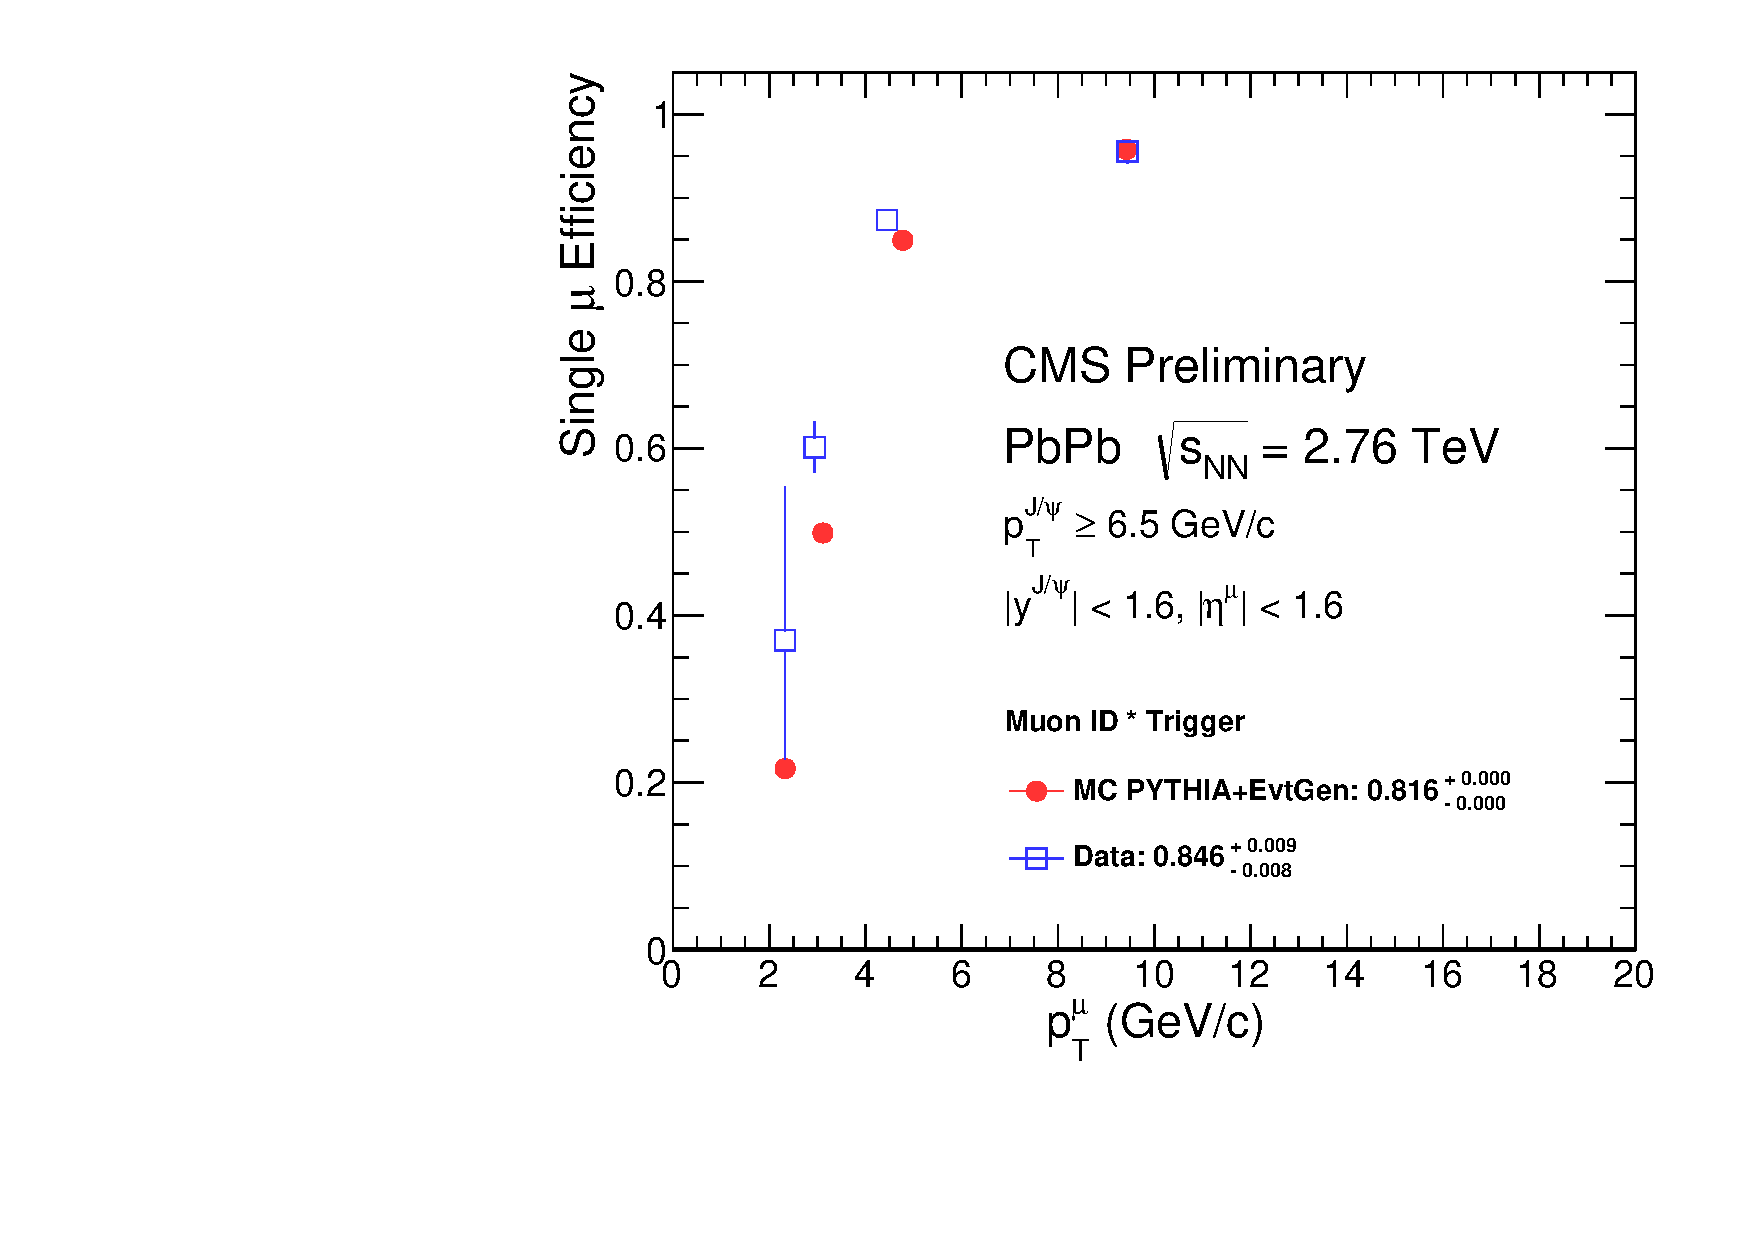
\includegraphics[width=0.45\textwidth]{Chapters/aCorrection/MuIdTrg2_Comp_HI_pt_RD_MC.pdf}
    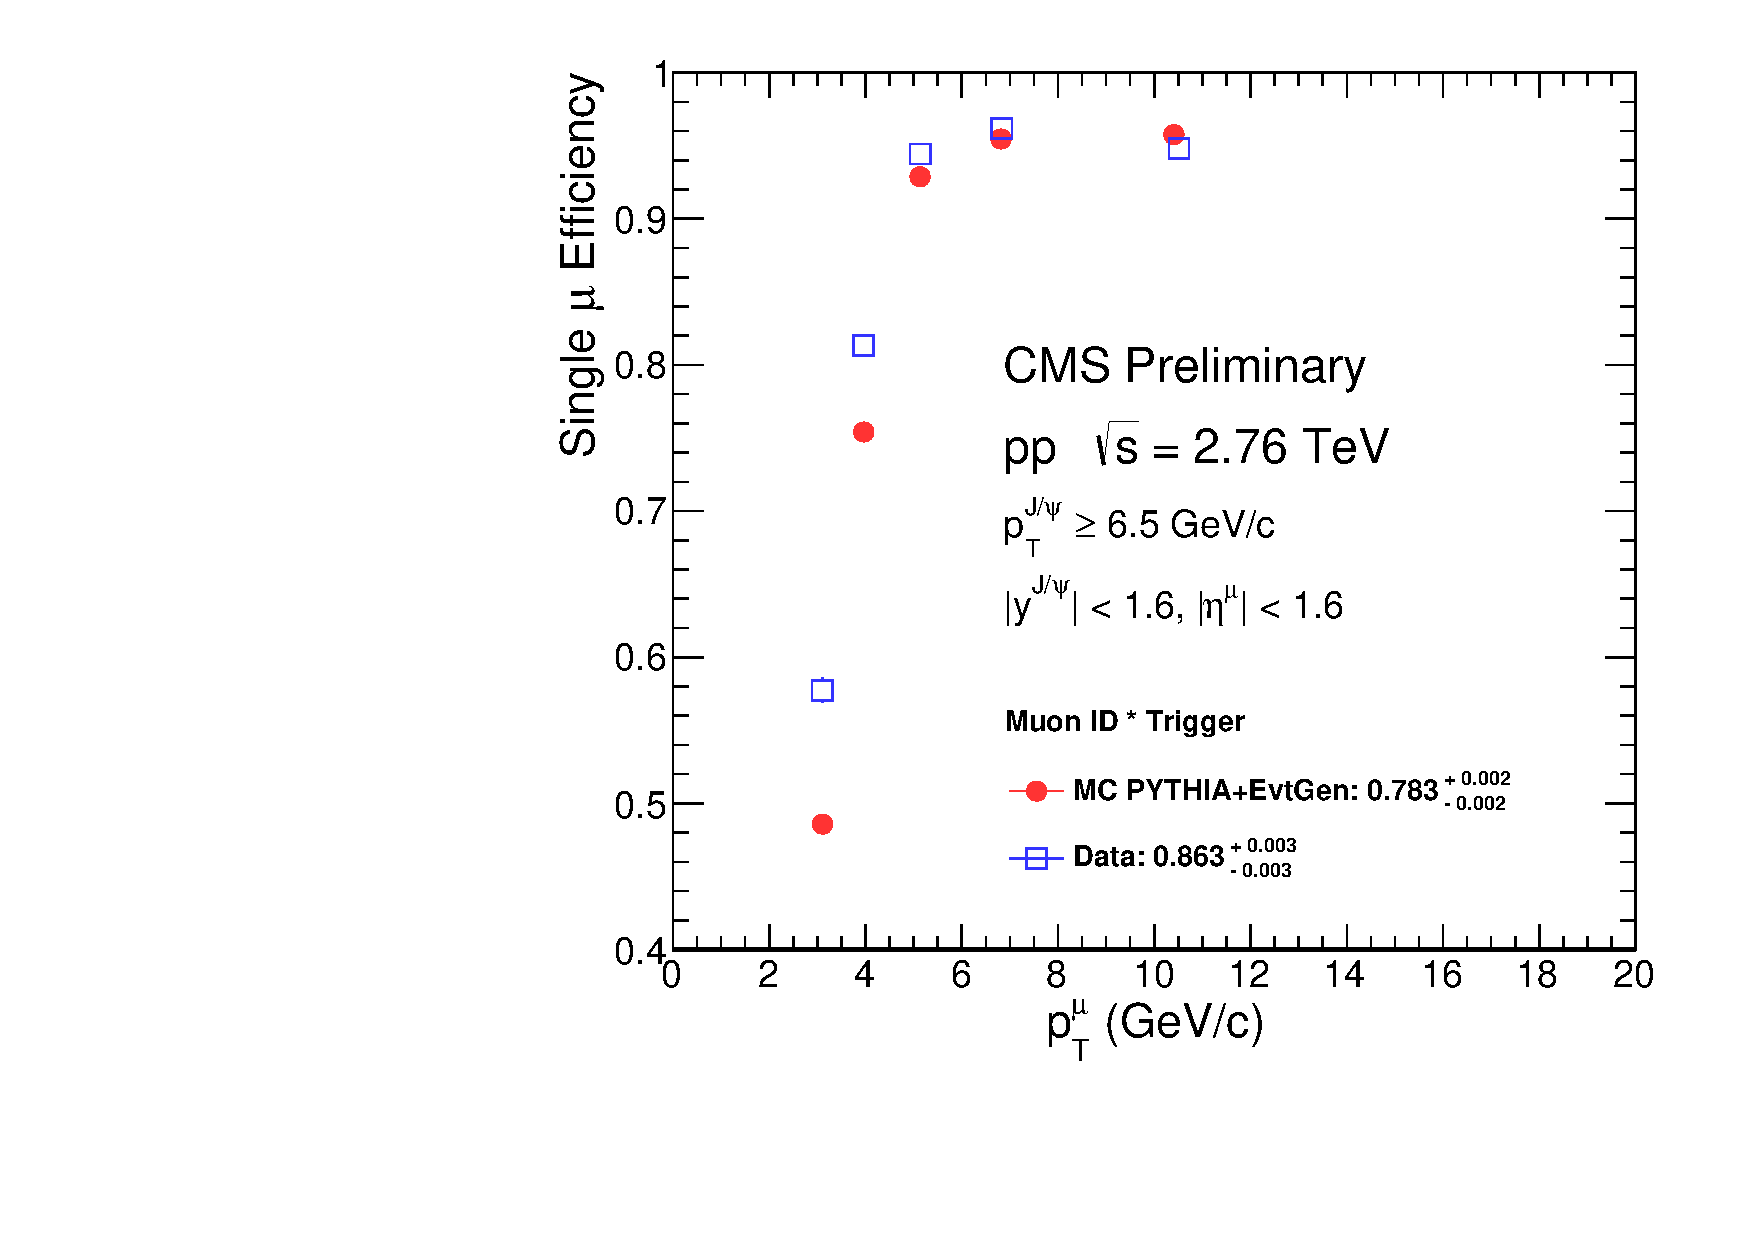
\includegraphics[width=0.45\textwidth]{Chapters/aCorrection/MuIdTrg2_Comp_pp_pt_RD_MC.pdf}
    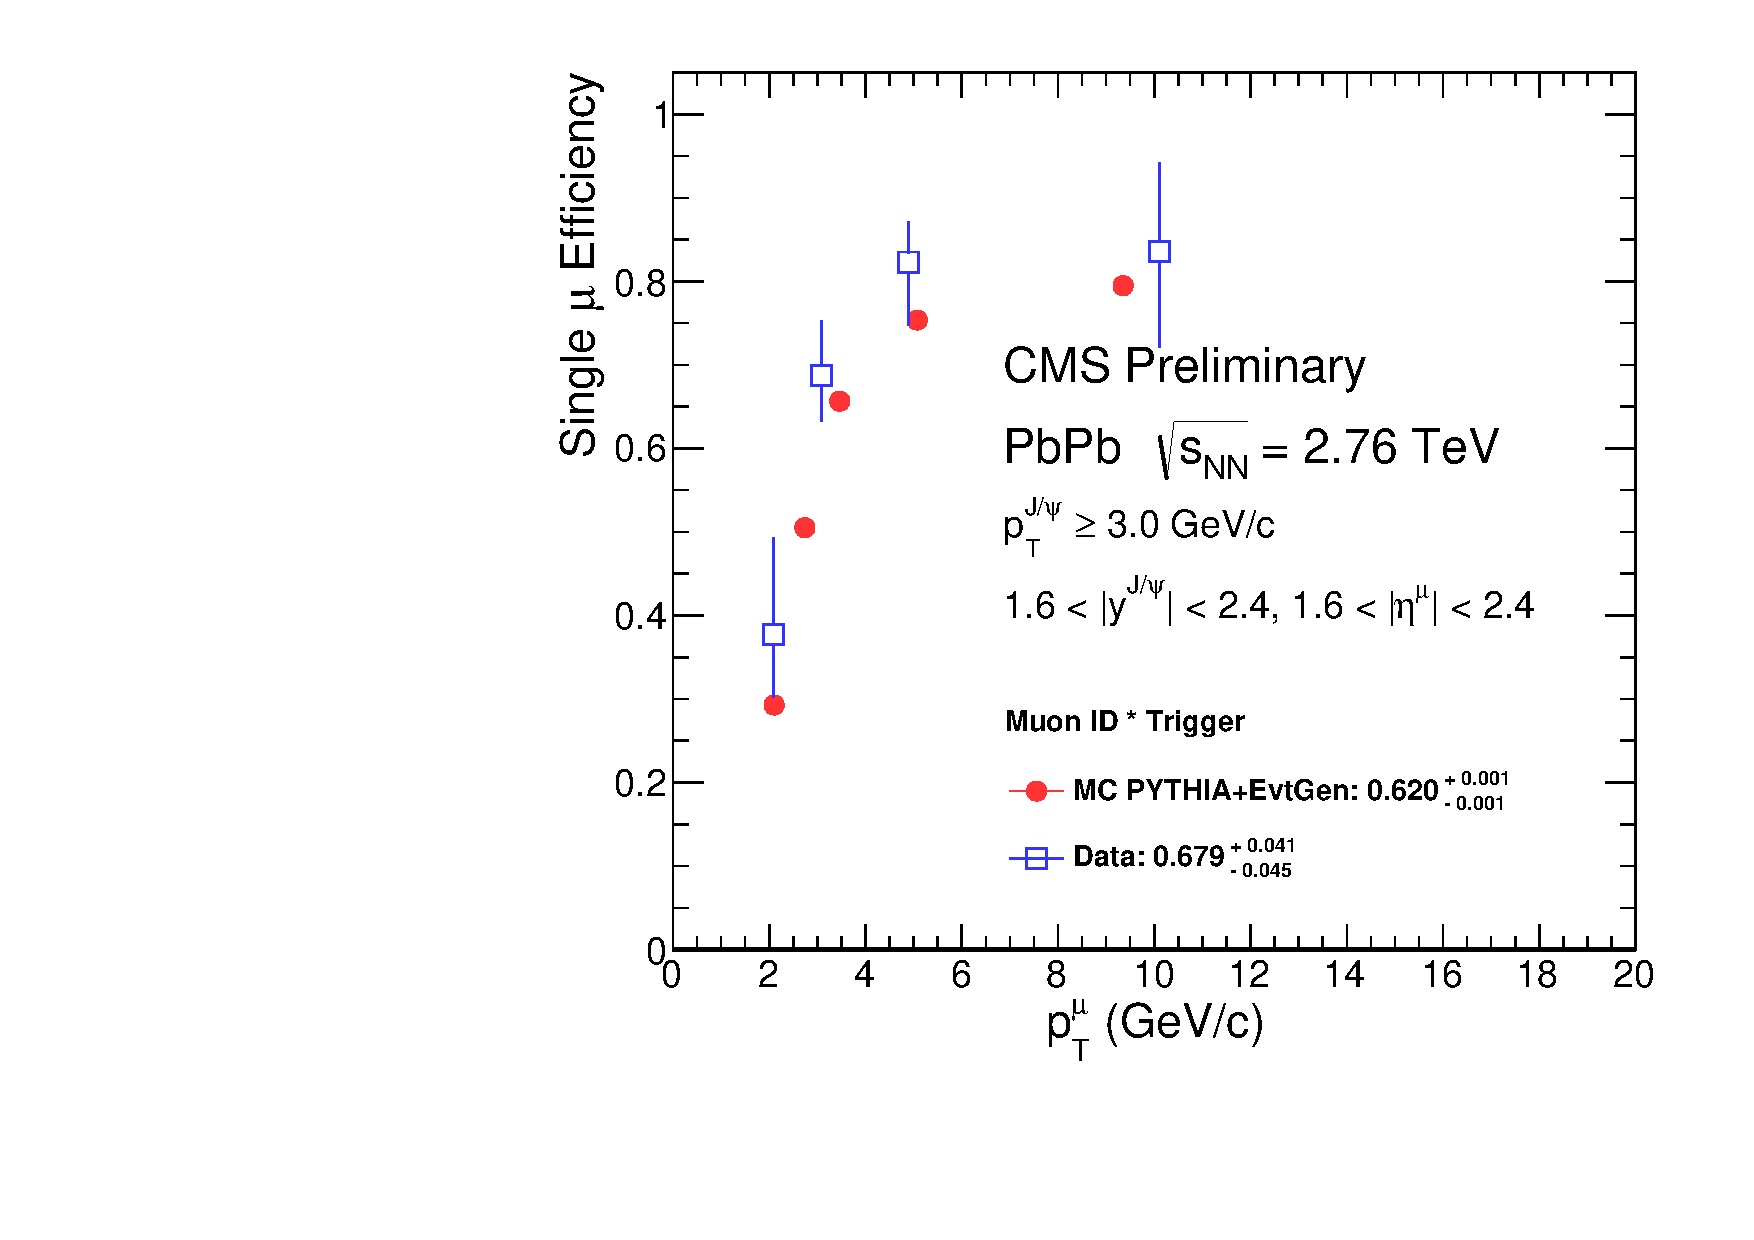
\includegraphics[width=0.45\textwidth]{Chapters/aCorrection/MuIdTrg3_Comp_HI_pt_RD_MC.pdf}
    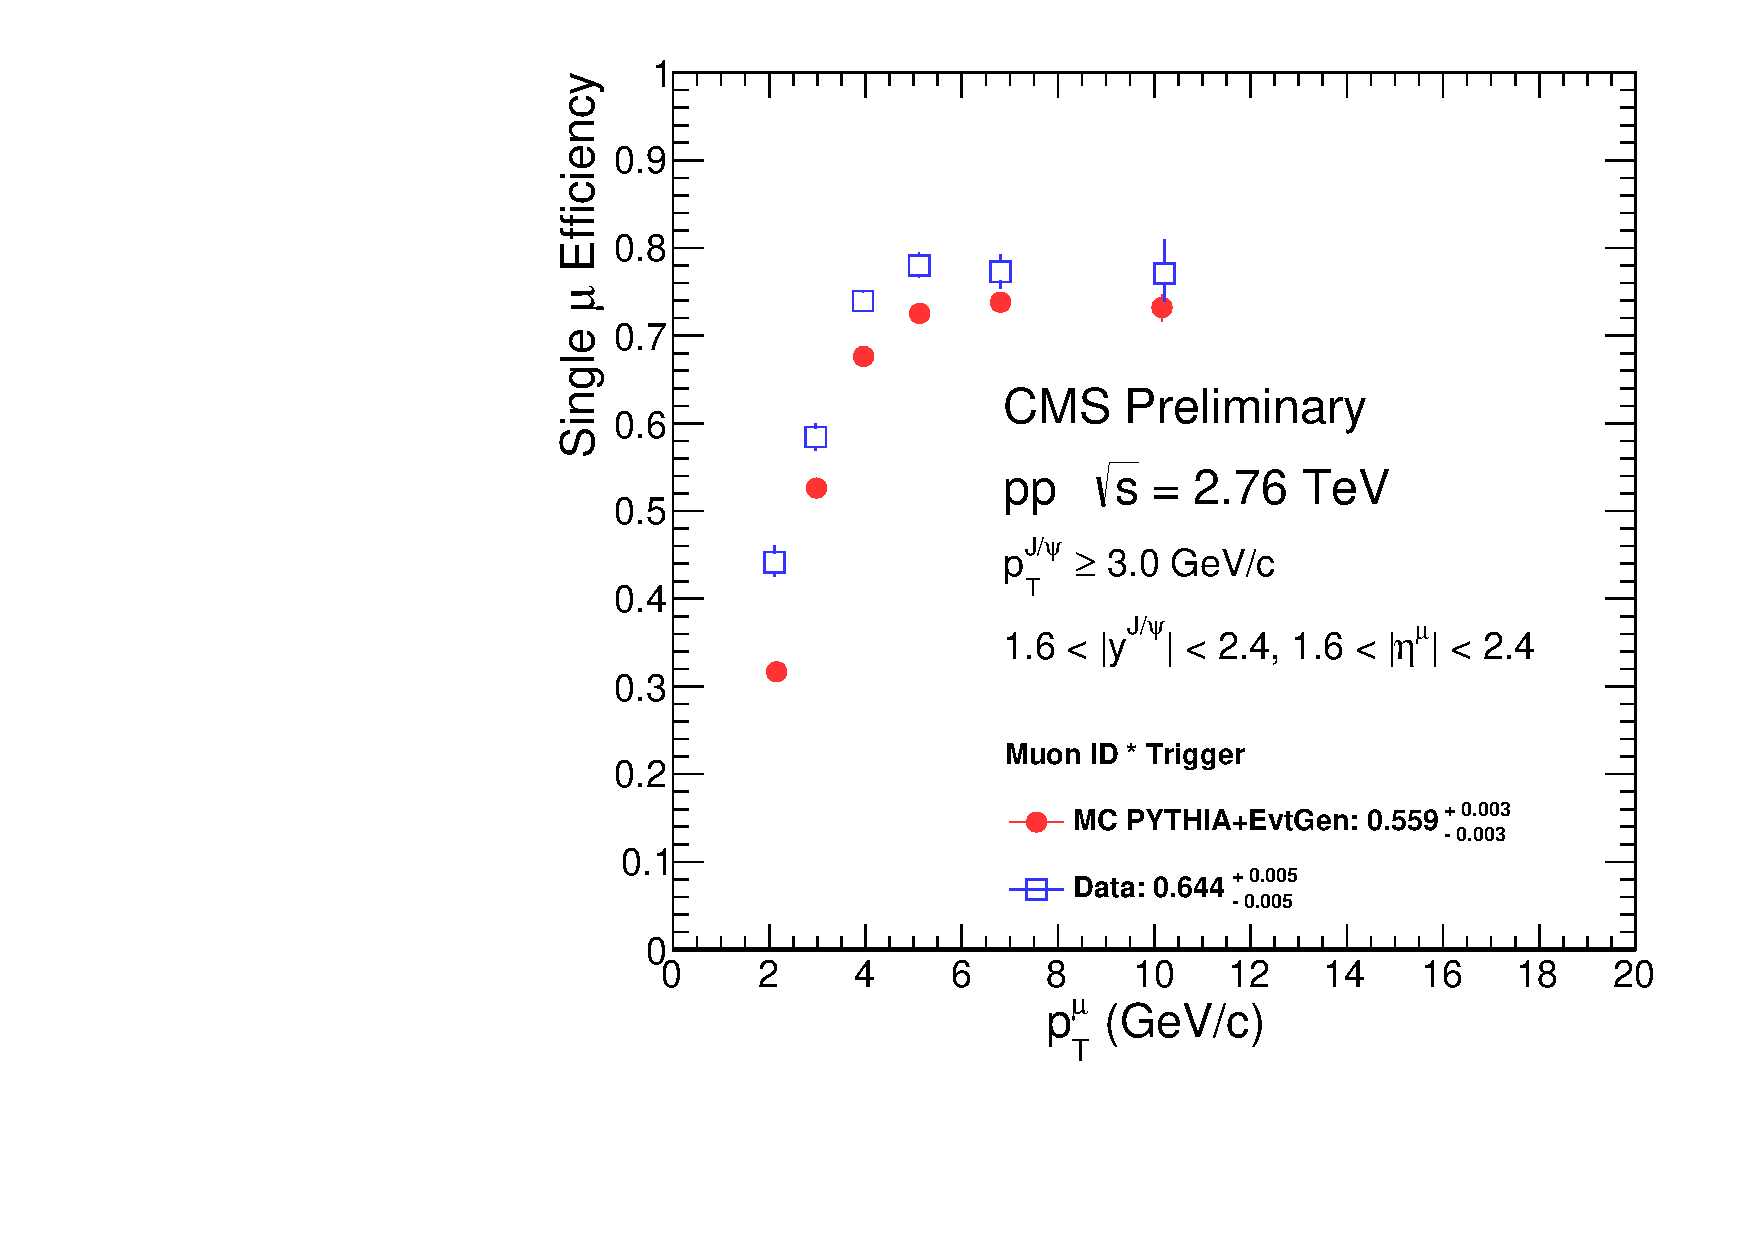
\includegraphics[width=0.45\textwidth]{Chapters/aCorrection/MuIdTrg3_Comp_pp_pt_RD_MC.pdf}
    \caption{Trigger and ID single muon efficiencies computed with the tag and
      probe method. Comparison between data \emph{(open blue squares)} and MC
      \emph{(red full circles)}.
      Top, left: efficiencies in the barrel using PbPb data and MC. Top,
      right: efficiencies in the barrel using pp data and MC.
      Bottom, left: efficiencies in the endcaps using PbPb data and MC.
      Bottom, right: efficiencies in the endcaps using pp data and MC.}
    \label{fig:trigid_eff}
  \end{center}
\end{figure}

First of all, we see a clear difference in the overall efficiencies
between endcaps and barrel pseudorapidities. This motivated the
splitting of our data in the first place, to get a consistent
correction for various detector areas. Second, there is an obvious
difference in performance between the PbPb and pp cases. Still, it is worth noting that in both cases, our
reconstruction, trigger and identification strategy is efficient down
to the lowest \pt\ muons kept in our analysis (muon \pt > 3.5 \GeVc).
Finally, and maybe most importantly, there are consistently some
relatively small differences between data and MC, which justify the
second-order corrections that we are trying to compute from single
muons.

%pp trigId_eta, pp trigId_pt
%AA trigId_eta, AA trigId_pt AA trigId_cent
\subsubsection*{Tracking efficiency in pp, PbPb collisions}
\label{subsec:def_tracking}
\begin{itemize}
\item Inner track reconstruction efficiency (including the inner to
  outer track matching efficiency) and track (inner and global) quality selection within the single muon acceptance cut defined in Section~\ref{sec:sigext_fits}:
  \begin{itemize}
  \item probe: a standalone muon (the four-momentum information is taken from the
    standalone part exclusively)
  \item passing probe: probe that is a global muon passing all track quality cuts.
  \end{itemize}

\end{itemize}

In the following Figure~\ref{fig:trk_eff_pp}, the resulting
single muon tracking efficiencies from $pp$ (data and MC) are
presented. We can see that the tracking efficiencies in data and
MC are consistent within uncertainties. As a result, it was
decided not to correct for possible discrepancies in this part of the
efficiency. The Muon Object Group (later called 'Muon POG') of CMS has
suggested us for this preliminary result to use a conservative
systematic uncertainty of 1.7\% per track, which is applied to the
final efficiency (twice, since there are two muons). For the final
version of this analysis, a thorough study of the track reconstruction
and inner to outer track matching sequences is being carried, and is not presented here.%  The
% aim of this study is to reduce discrepancies, the pp efficiencies
% being generally much closer to 1 for the tracking part.

\begin{figure}
  \begin{center}
    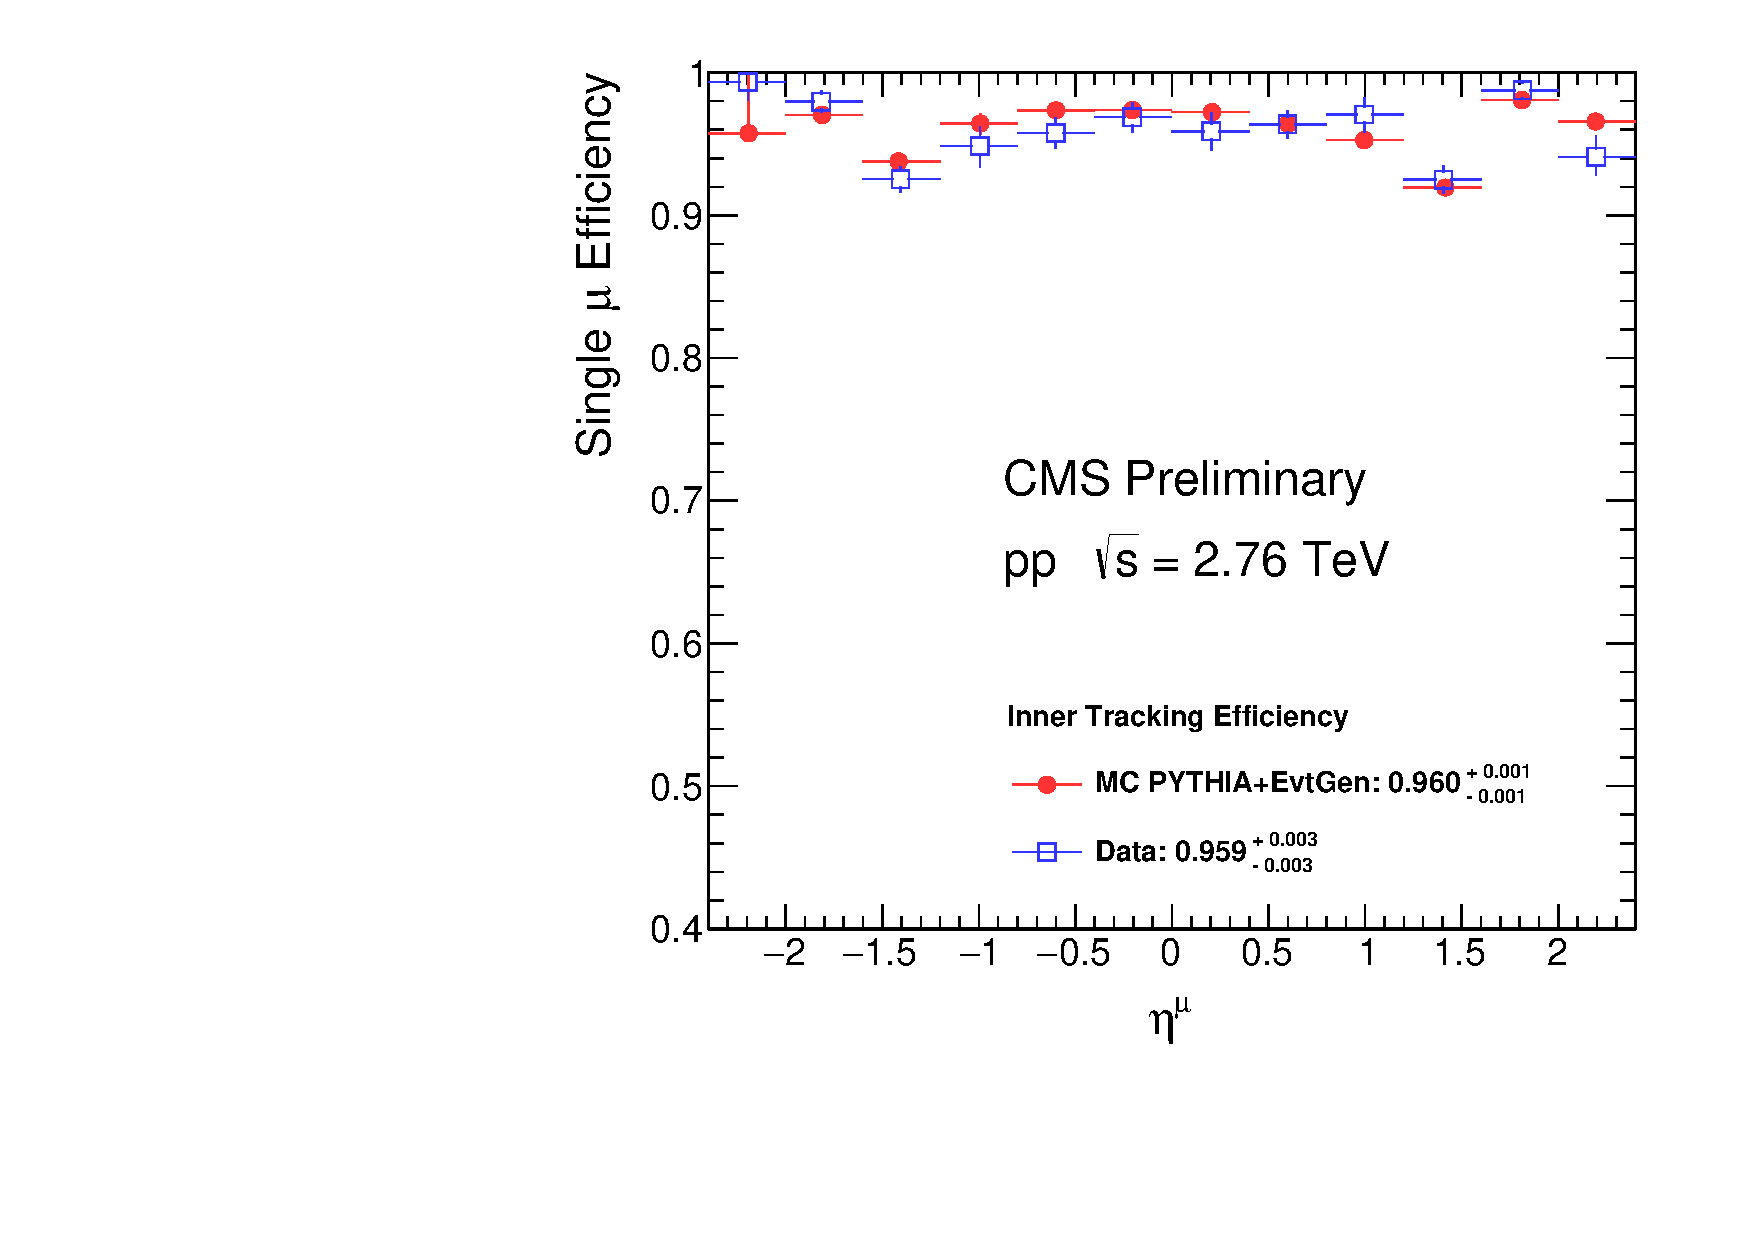
\includegraphics[width=0.45\textwidth]{Chapters/aCorrection/Trk_Comp_pp_eta_RD_MC.pdf}
    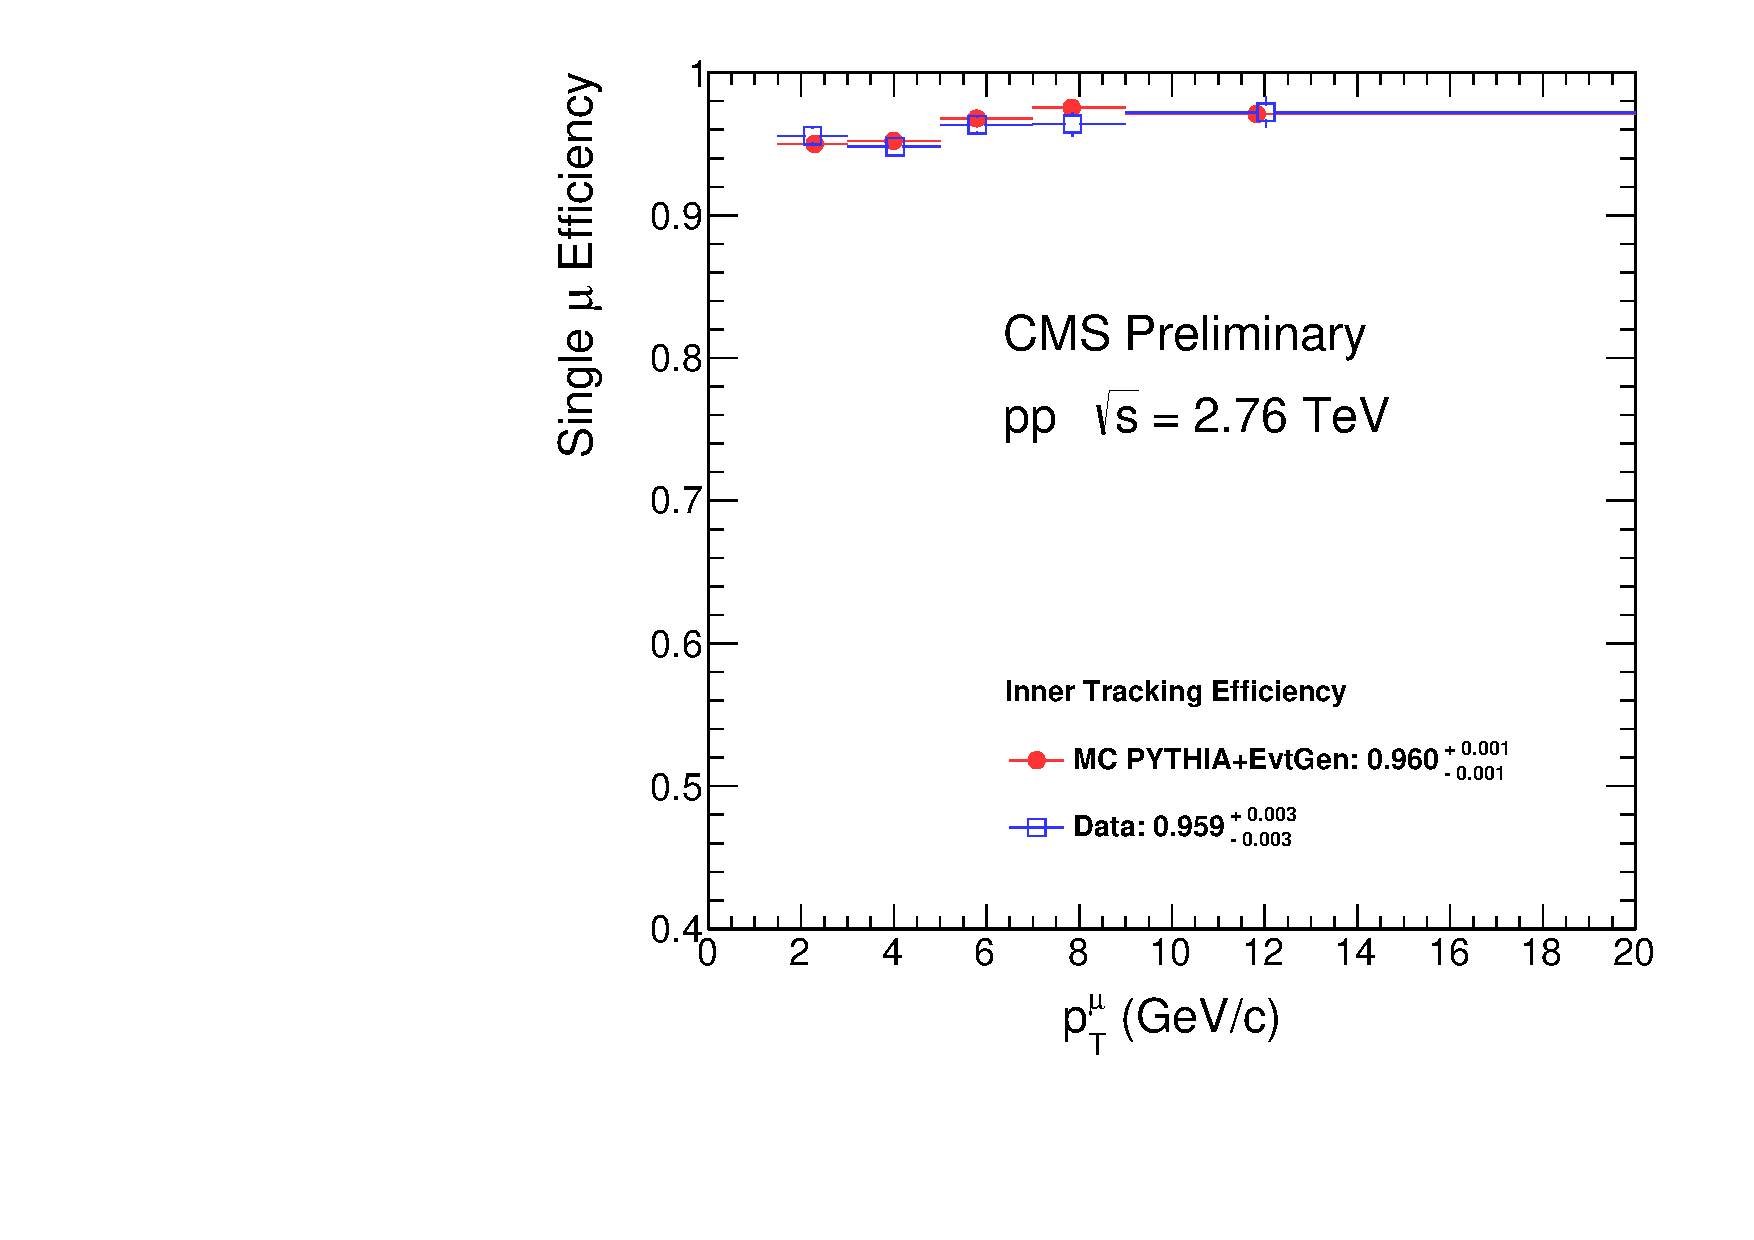
\includegraphics[width=0.45\textwidth]{Chapters/aCorrection/Trk_Comp_pp_pt_RD_MC.pdf}
%
    \caption{
      pp tracking and track matching efficiencies computed with tag and
      probe. Comparison between data \emph{(open blue squares)} and MC
      \emph{(red full circles)}.
      Left: efficiencies in pp data and MC \vs. probe pseudo-rapdity.
      Right: efficiencies in pp data and MC \vs. probe \pt.
    }
    \label{fig:trk_eff_pp}
  \end{center}
\end{figure}

Figure~\ref{fig:trk_eff_HI}, shows the resulting
single muon tracking efficiencies from PbPb are
presented. Generally speaking, the integrated data and MC efficiencies
seem to disagree. Large uncertainties appear in the $\eta$-binned plot, for the
data efficiencies, and the lowest-\pt bin does not enter our
analysis. Nonetheless, it is good to see that tracking efficiencies do not
depend on the multiplicity in the event, confirming that the tracking
works well up to the most central PbPb collisions.

%We can see that the tracking efficiencies in pp(data) and
% pp(MC) are consistent within uncertainties. As a result, it was
% decided not to correct for possible discrepancies in this part of the
% efficiency.
Upon various consultations with the Muon POG of
CMS, it was decided to opt for a conservative 5\% systematic
uncertainty per track instead of assigning a correction, for this
preliminary result, while we investigate more on the nature of this underperformance.

\begin{figure}
  \begin{center}
    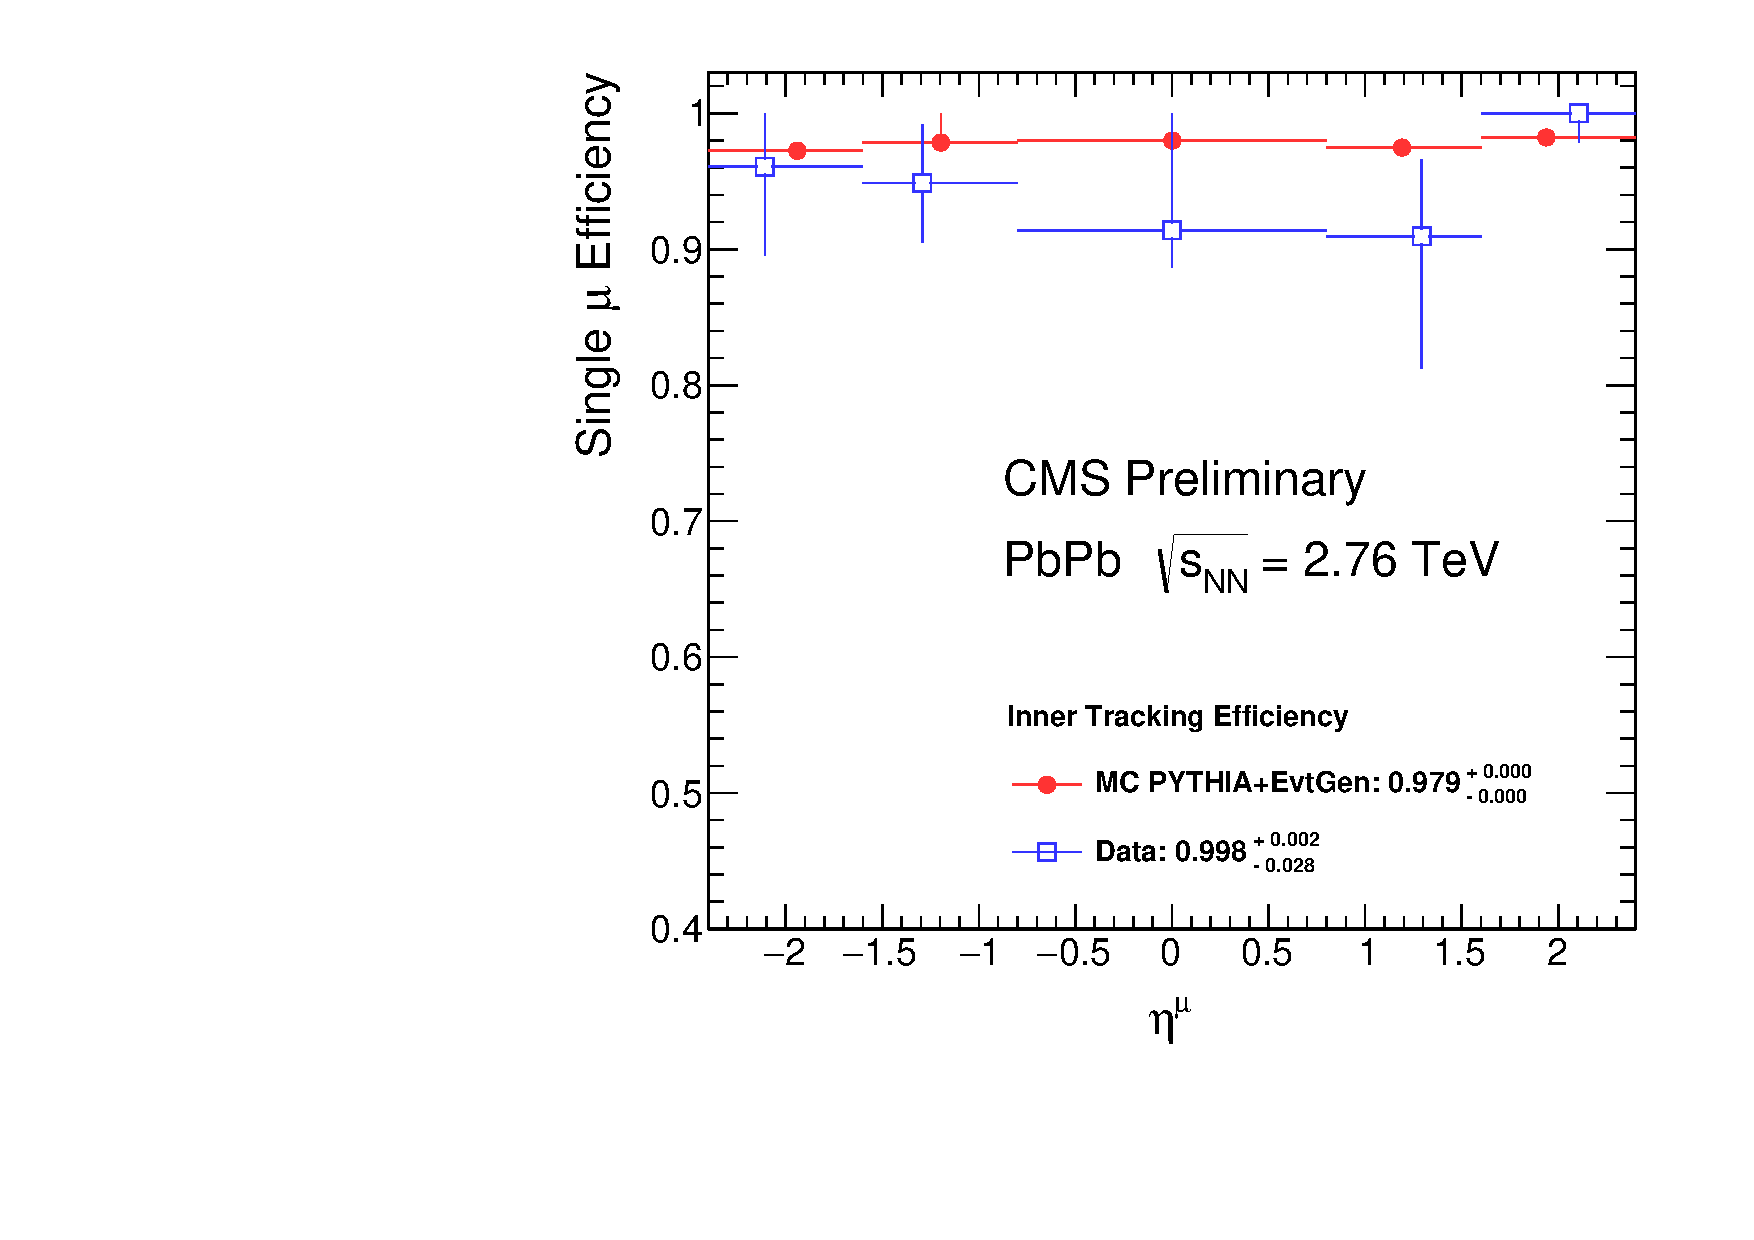
\includegraphics[width=0.45\textwidth]{Chapters/aCorrection/Trk_Comp_HI_eta_RD_MC.pdf}
    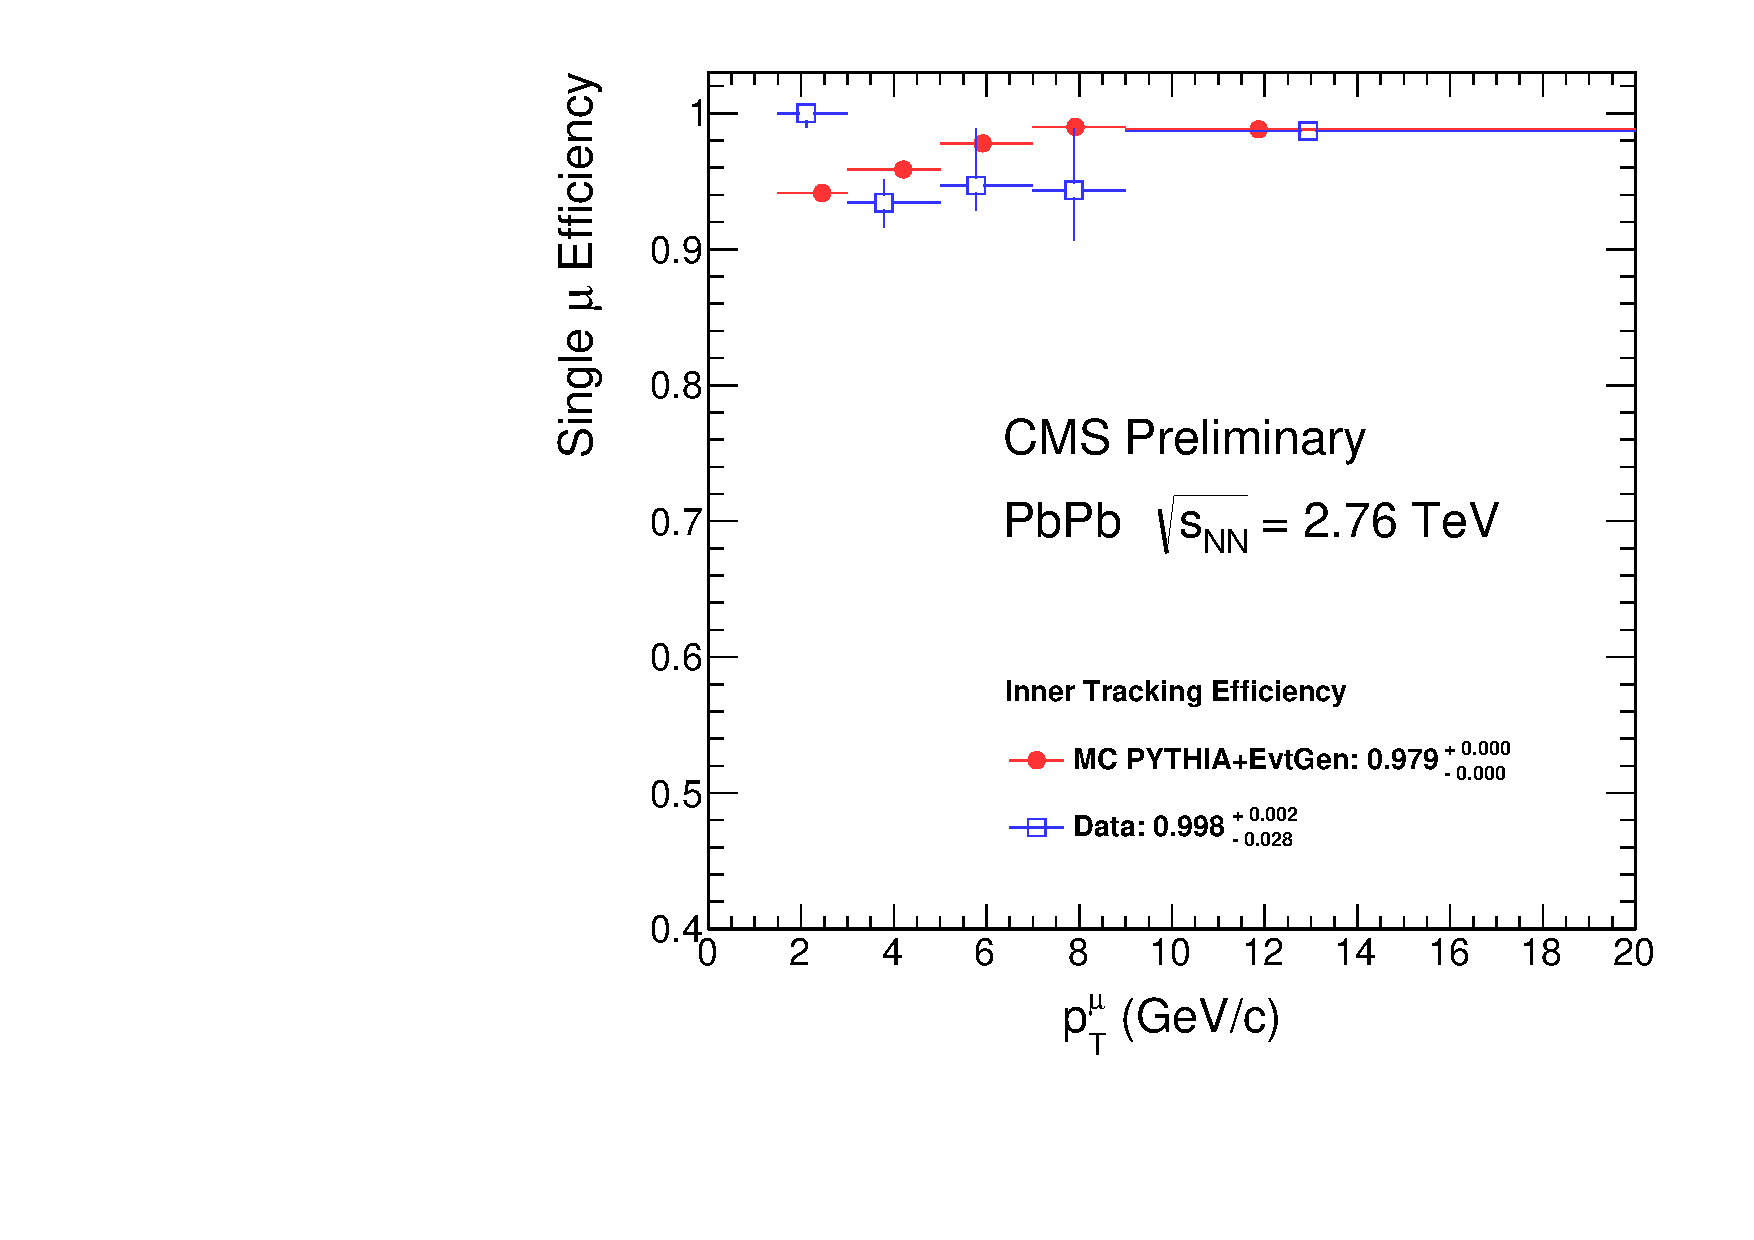
\includegraphics[width=0.45\textwidth]{Chapters/aCorrection/Trk_Comp_HI_pt_RD_MC.pdf}
    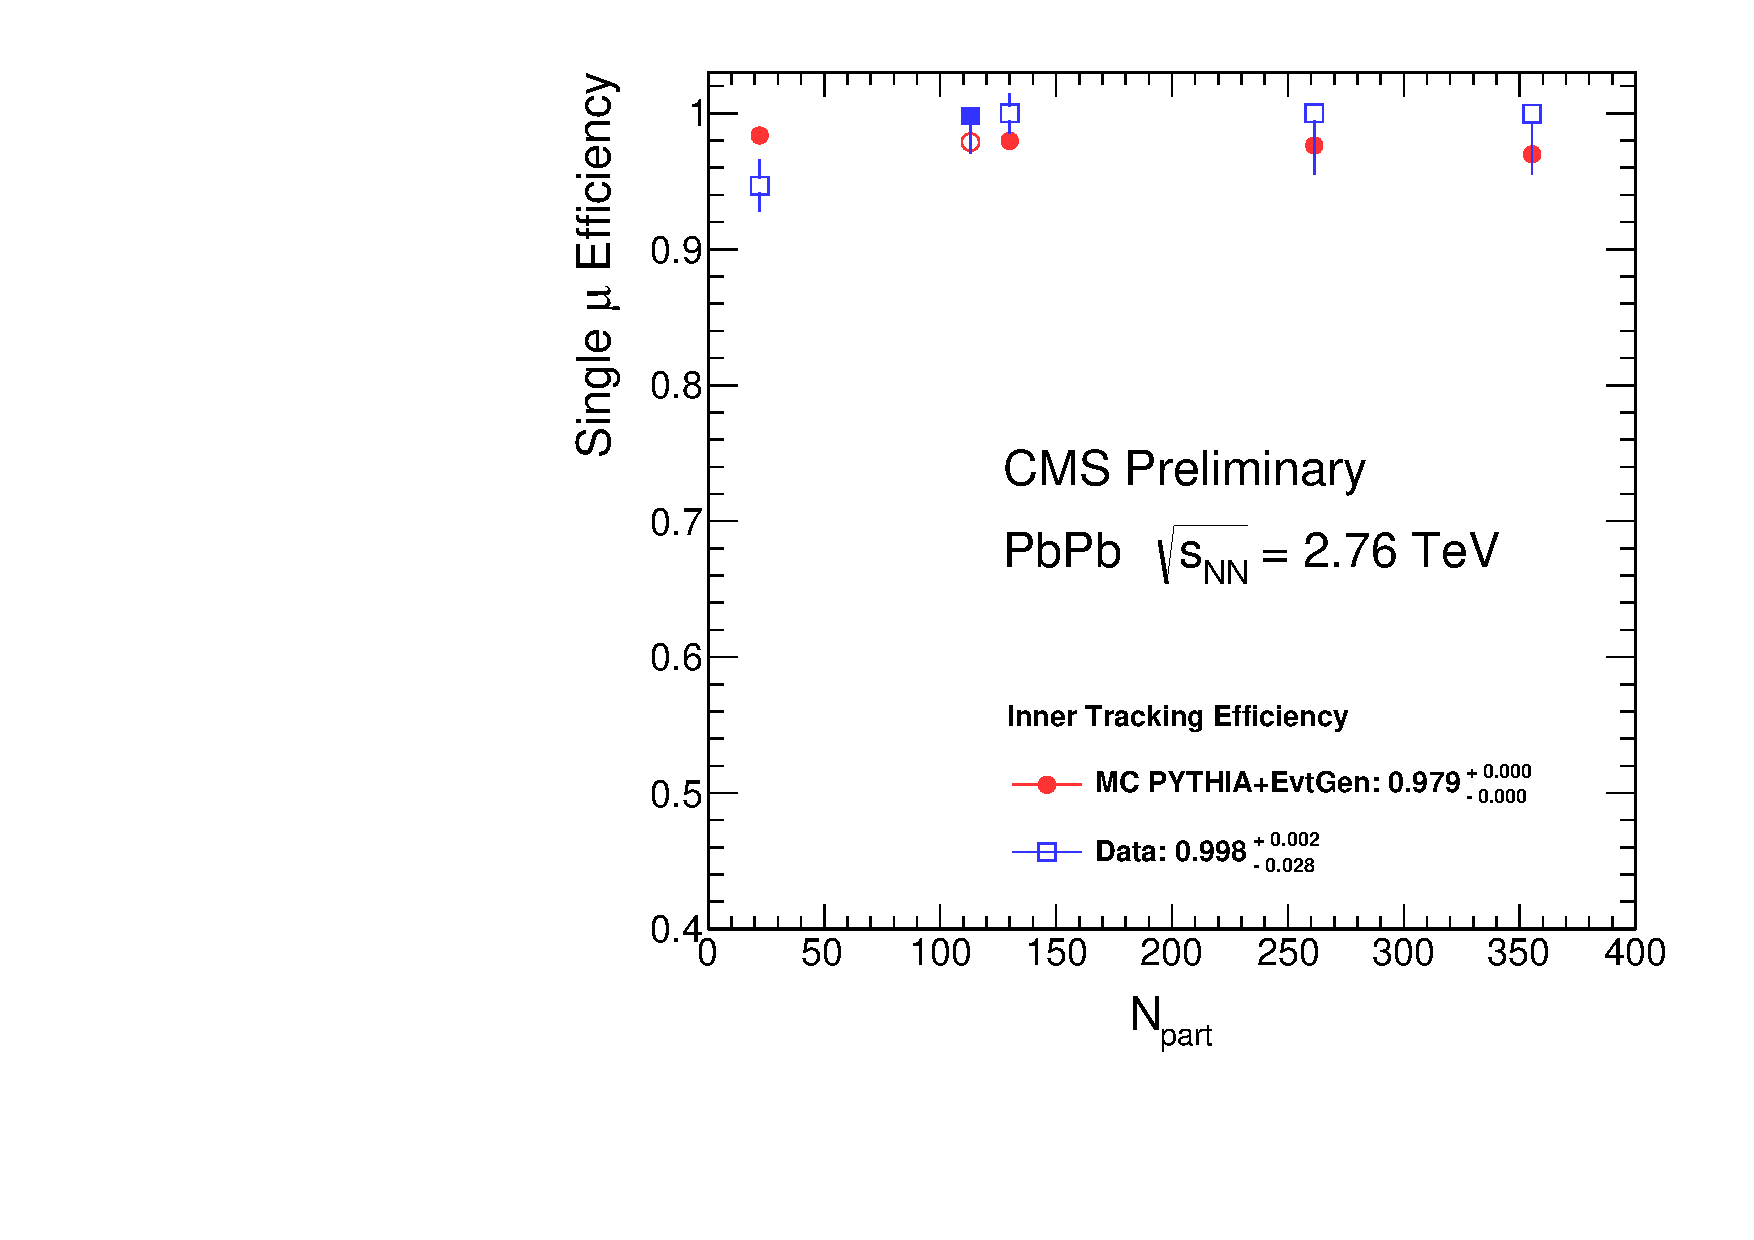
\includegraphics[width=0.45\textwidth]{Chapters/aCorrection/Trk_Comp_HI_CNT_RD_MC.pdf}
    \caption{
      PbPb Tracking and track matching efficiencies computed with tag and
      probe. Comparison between data \emph{(open blue squares)} and MC
      \emph{(red full circles)}.
      Left: efficiencies in PbPb data and MC \vs. probe pseudo-rapdity.
      Right: efficiencies in PbPb data and MC \vs. probe \pt.
      Bottom: efficiencies in PbPb data and MC \vs. probe \pt.
    }
    \label{fig:trk_eff_HI}
  \end{center}
\end{figure}

%pp trk_eta, pp trk_pt
%AA trk_eta, AA trk_pt AA trk_cent


\subsection{Correction to the dimuon efficiency}
\label{sec:tnp_dimueff}

In the previous paragraphs, I have presented the differences between
single muon efficiencies in MC and data, using the Tag and Probe
method on muons coming from \Jpsi. Now, let us try to go from the
discrepancies at single muon level to their effect on the dimuon efficiency. Since the efficiencies are
\pt-dependent, one can take the ratio \eff$^{data} / \eff^{MC}$ as a
function of the probe~\pt
\begin{equation}
\Ctnp  = \frac{\eff_{\mu}^{\rm data}(\rm trig|ID)}{{\eff_{\mu}^{\rm
      MC}(\rm trig|ID)}},
\label{eq:ctnp}
\end{equation}

where \Ctnp\ is a single-muon data-MC correction function. This
correction is only limited by the statistical accuracy of the
data sample, hence the main uncertainty will come from varying the
$\eff^{data}$ part. Figure~\ref{fig:ctnp_fits} (left) shows the single
muon efficiencies when probing the trigger+ID part, for the PbPb
forward sample (which is the part where corrections are the
largest). Both $\eff^{data}$ and $\eff^{MC}$ are fitted using an error
function, and the ratio \Ctnp\ is presented (right), with a fit to the
ratio of two error functions (red line), compared to the ratio of the
error functions fitted on the left (dashed line).

\begin{figure}[t]
  \begin{center}
    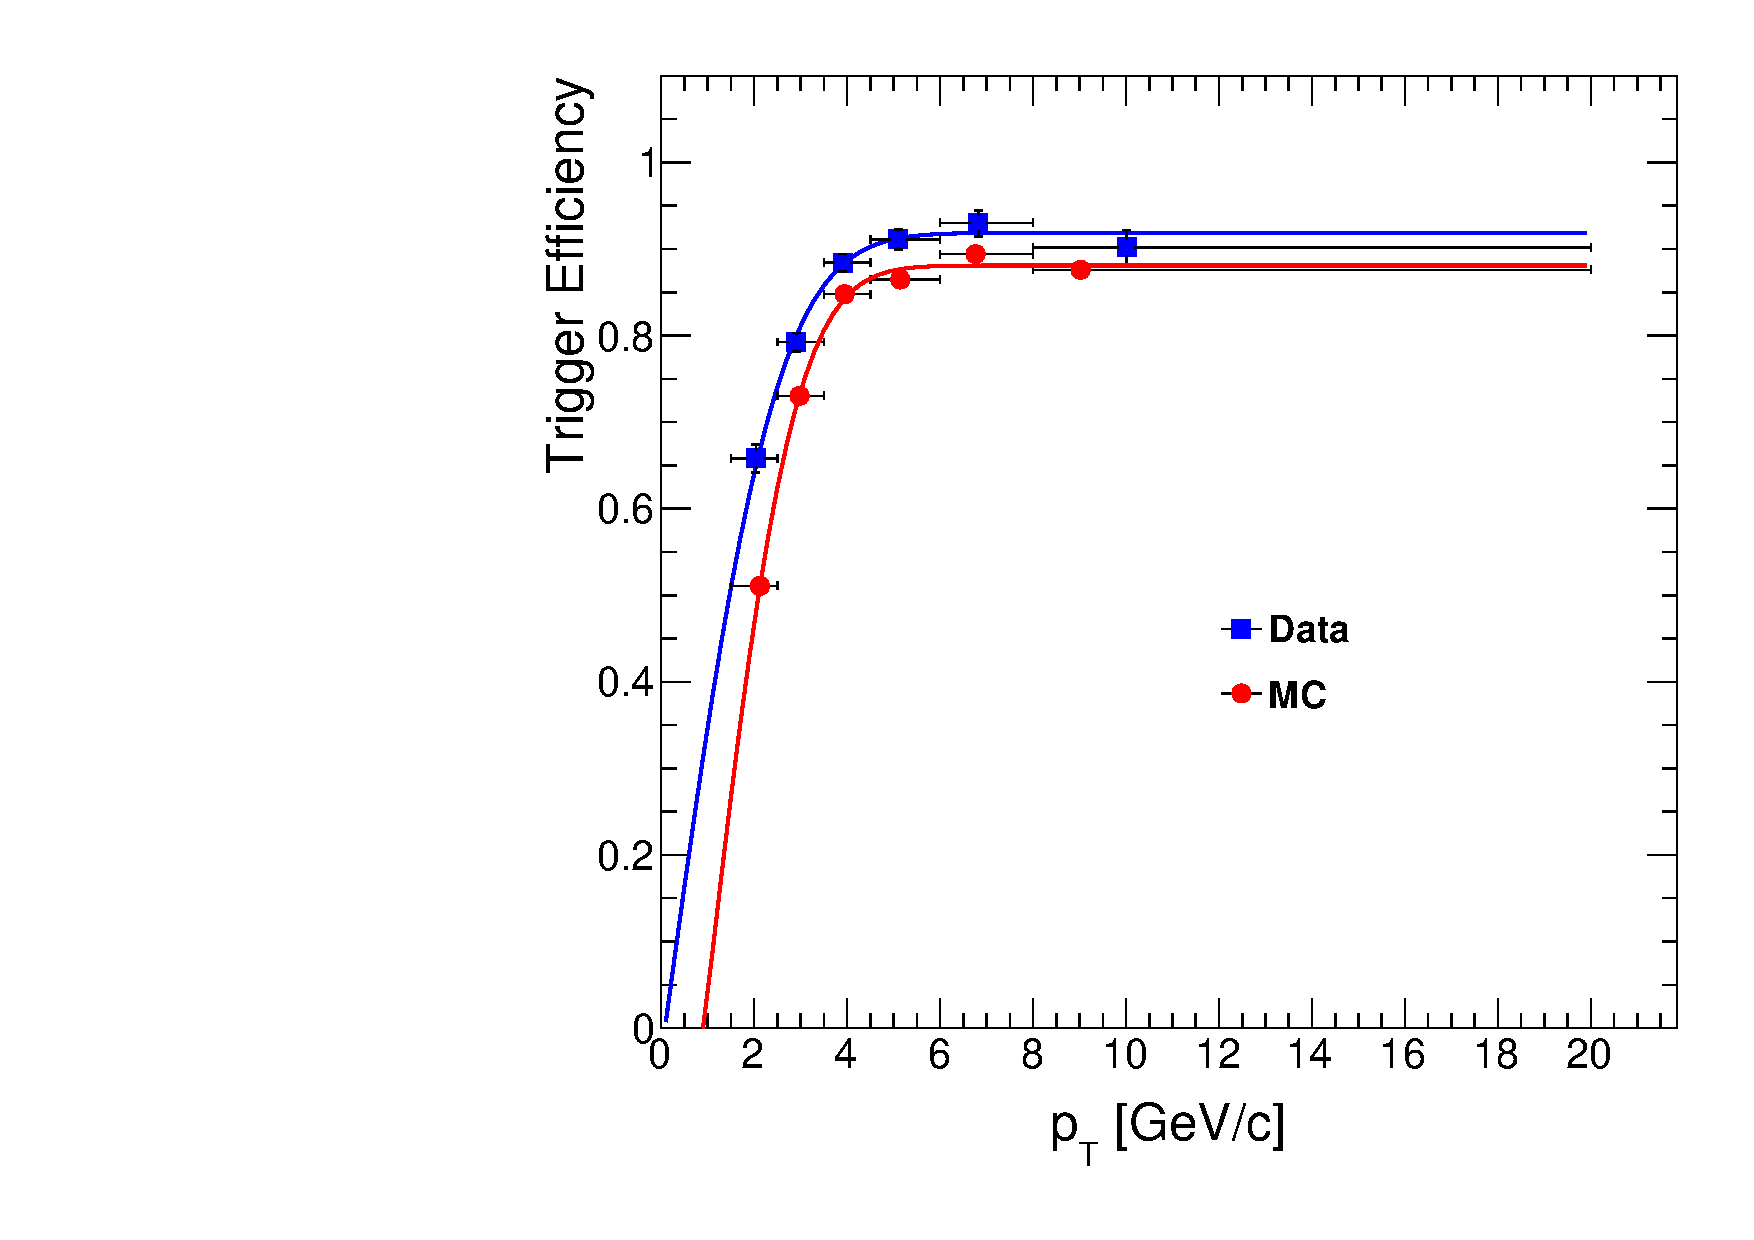
\includegraphics[width=0.4\textwidth]{Chapters/aCorrection/tnp_trig_eff_pbpb_forward.pdf}
    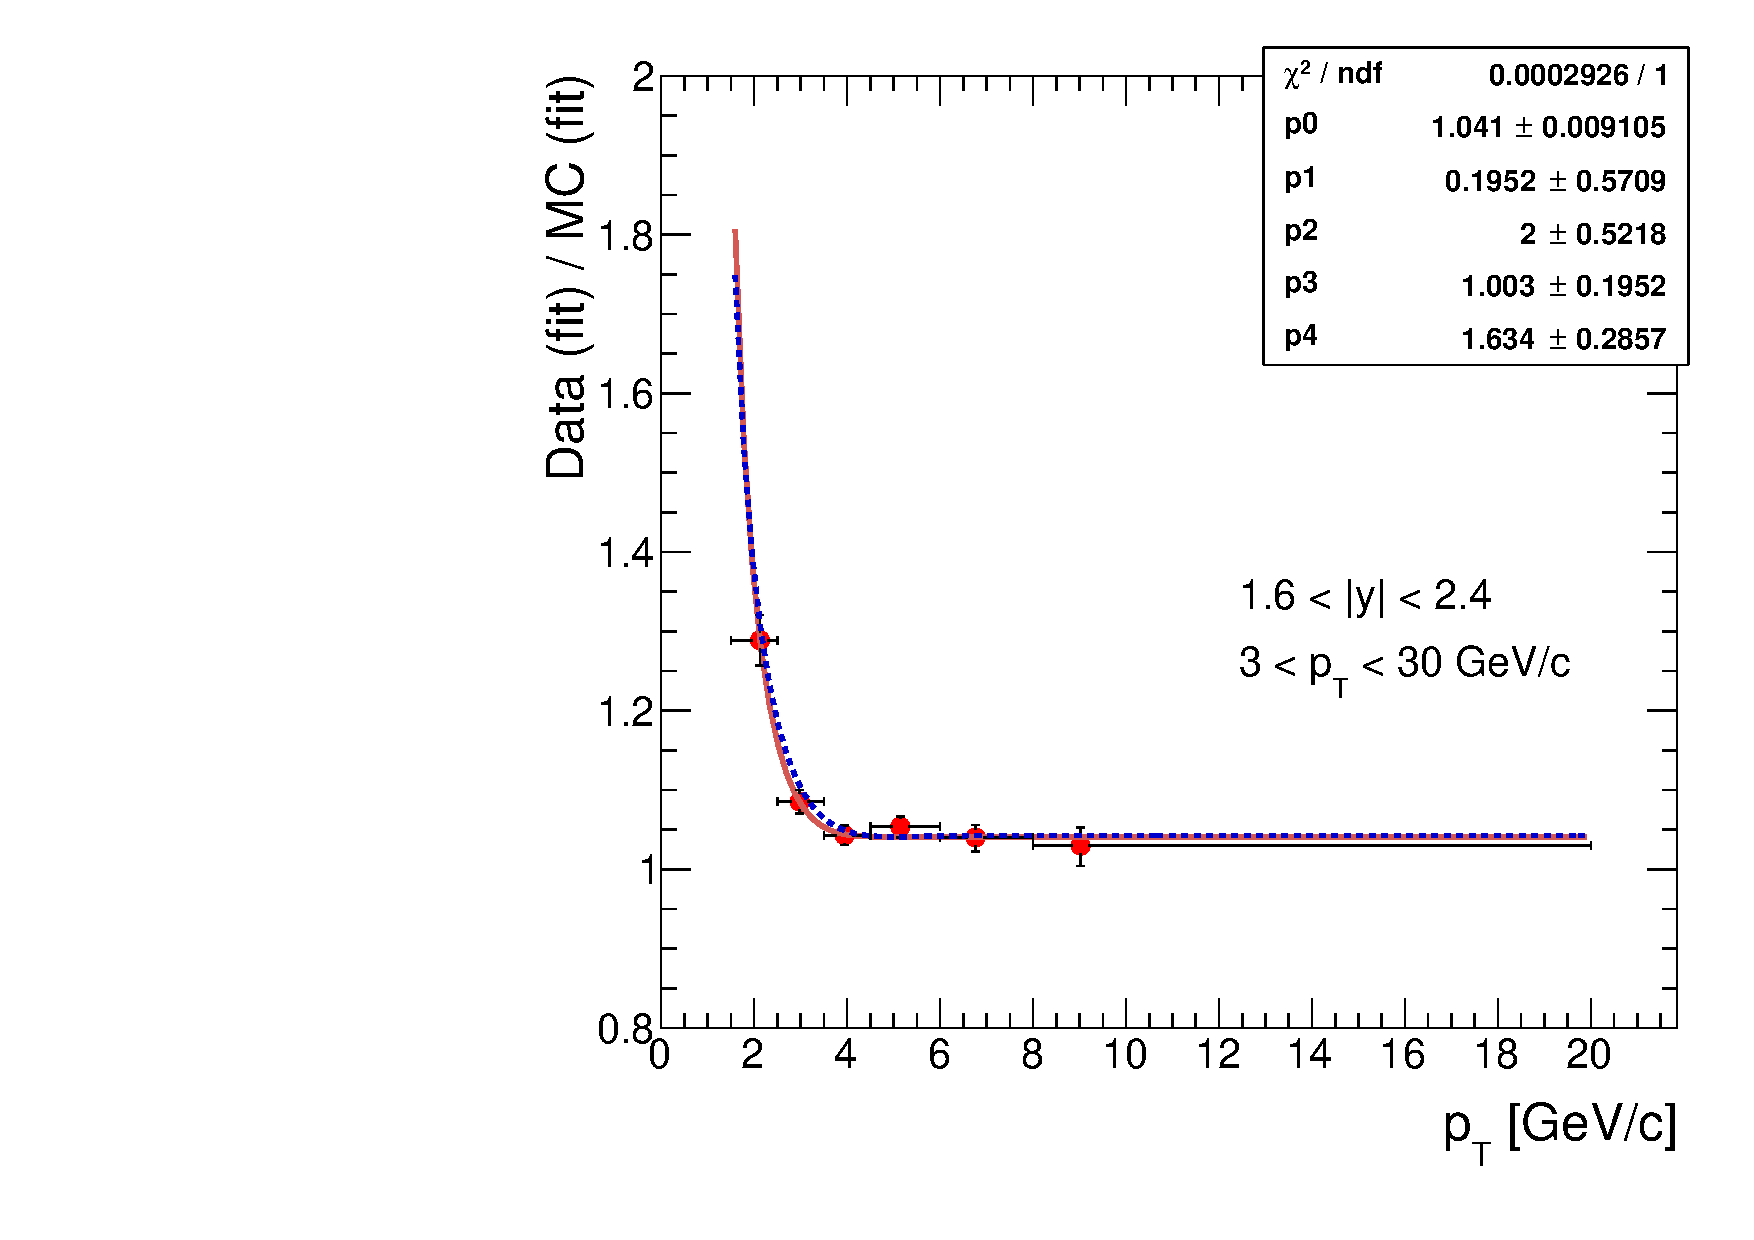
\includegraphics[width=0.4\textwidth]{Chapters/aCorrection/tnp_trig_eff_dataMC_Ratio_pbpb_forward.pdf}
    \caption{
      Left: single muon efficiencies in PbPb forward data and MC
      \vs. \pt. Both efficiencies are fitted to an error function.
      Right: single muon correction factor \Ctnp\ in PbPb forward
      data, as a function of probe-\pt. Reminder: muons below \pt = 3.5 \GeVc
      are not included in this analysis.
    }
    \label{fig:ctnp_fits}
  \end{center}
\end{figure}
By virtue of Equation~\ref{eq:ctnp}, \Ctnp\ is a continuous function of
\pt, differential (2 bins) in muon \Pgh. Figure~\ref{fig:SF} shows the \Ctnp\ functions for pp, barrel and
forward, and for PbPb, barrel and endcap regions .
\begin{figure}[h]
  \begin{center}
    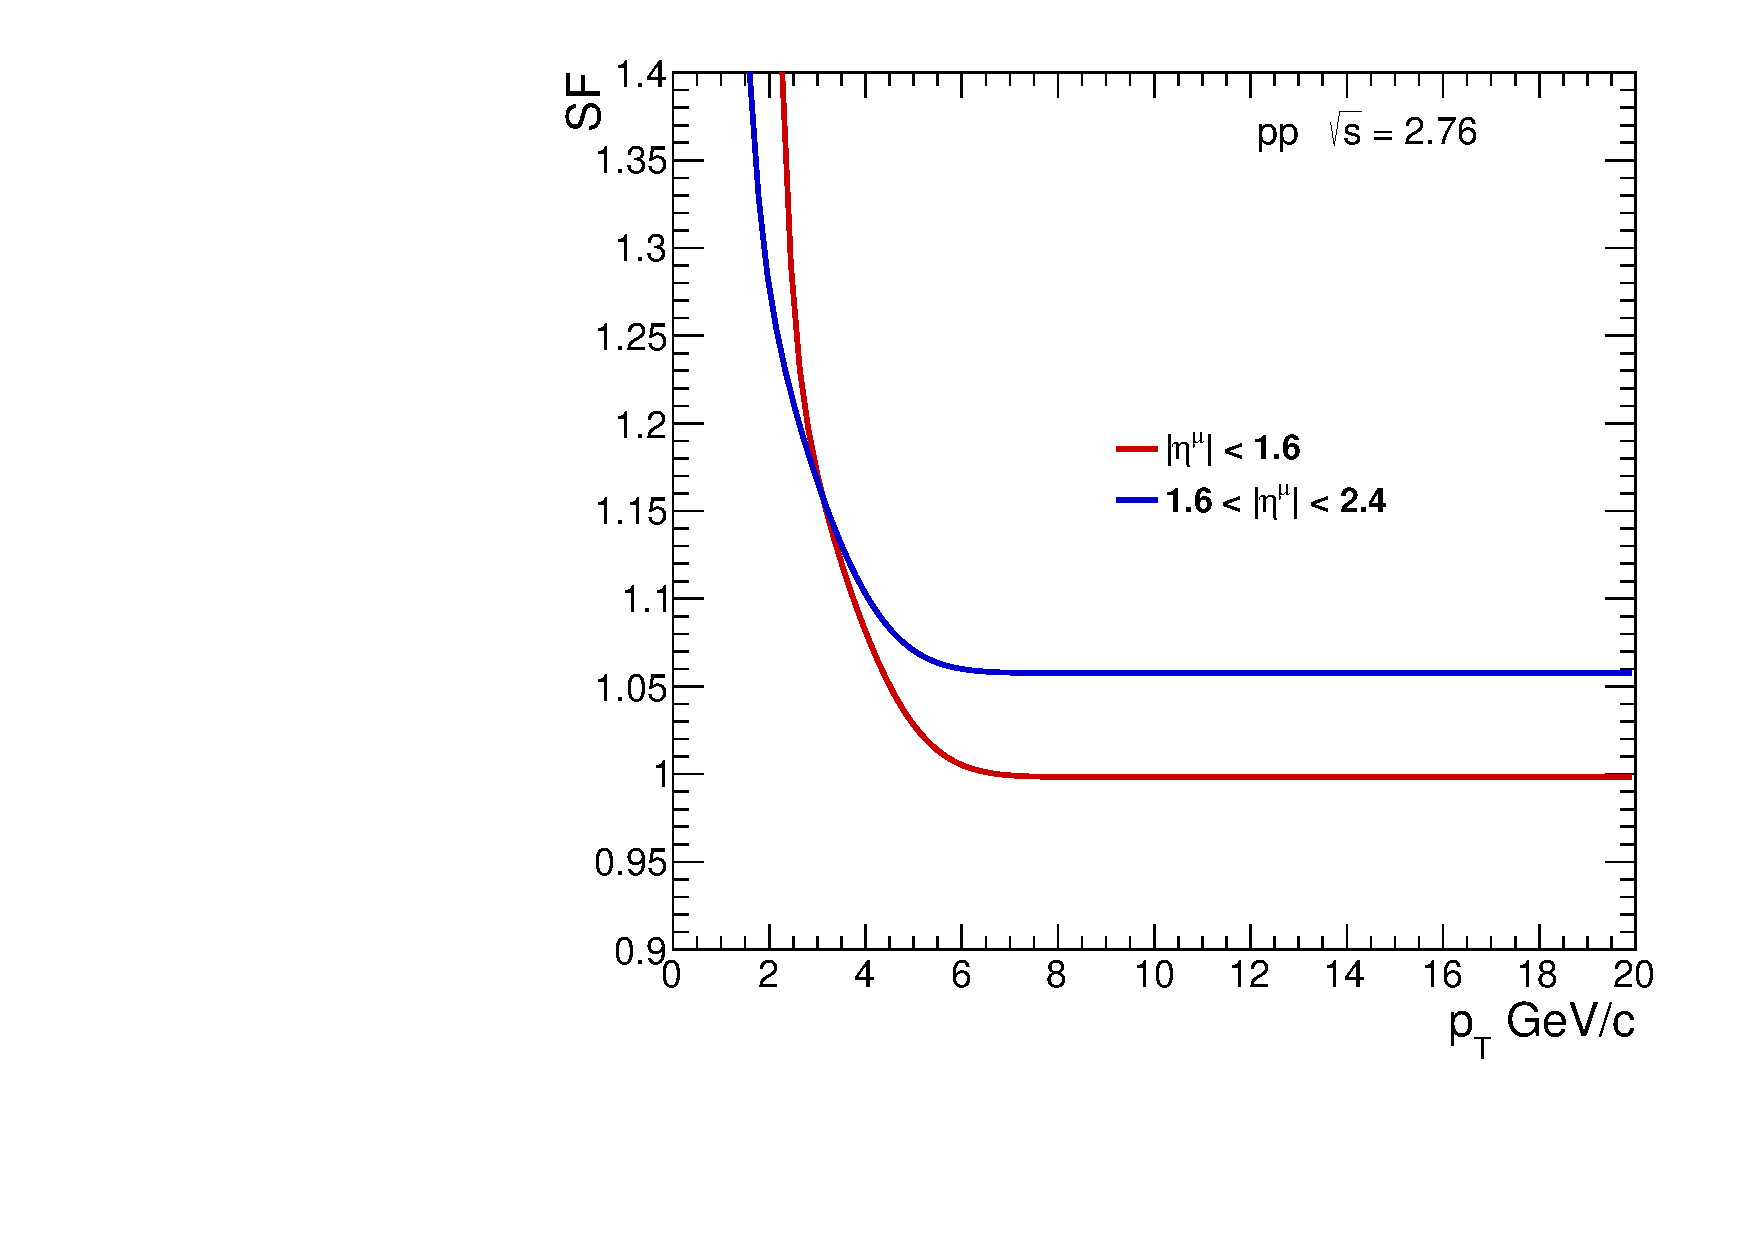
\includegraphics[width=0.4\textwidth]{Chapters/aCorrection/scale_factor_pp.pdf}
    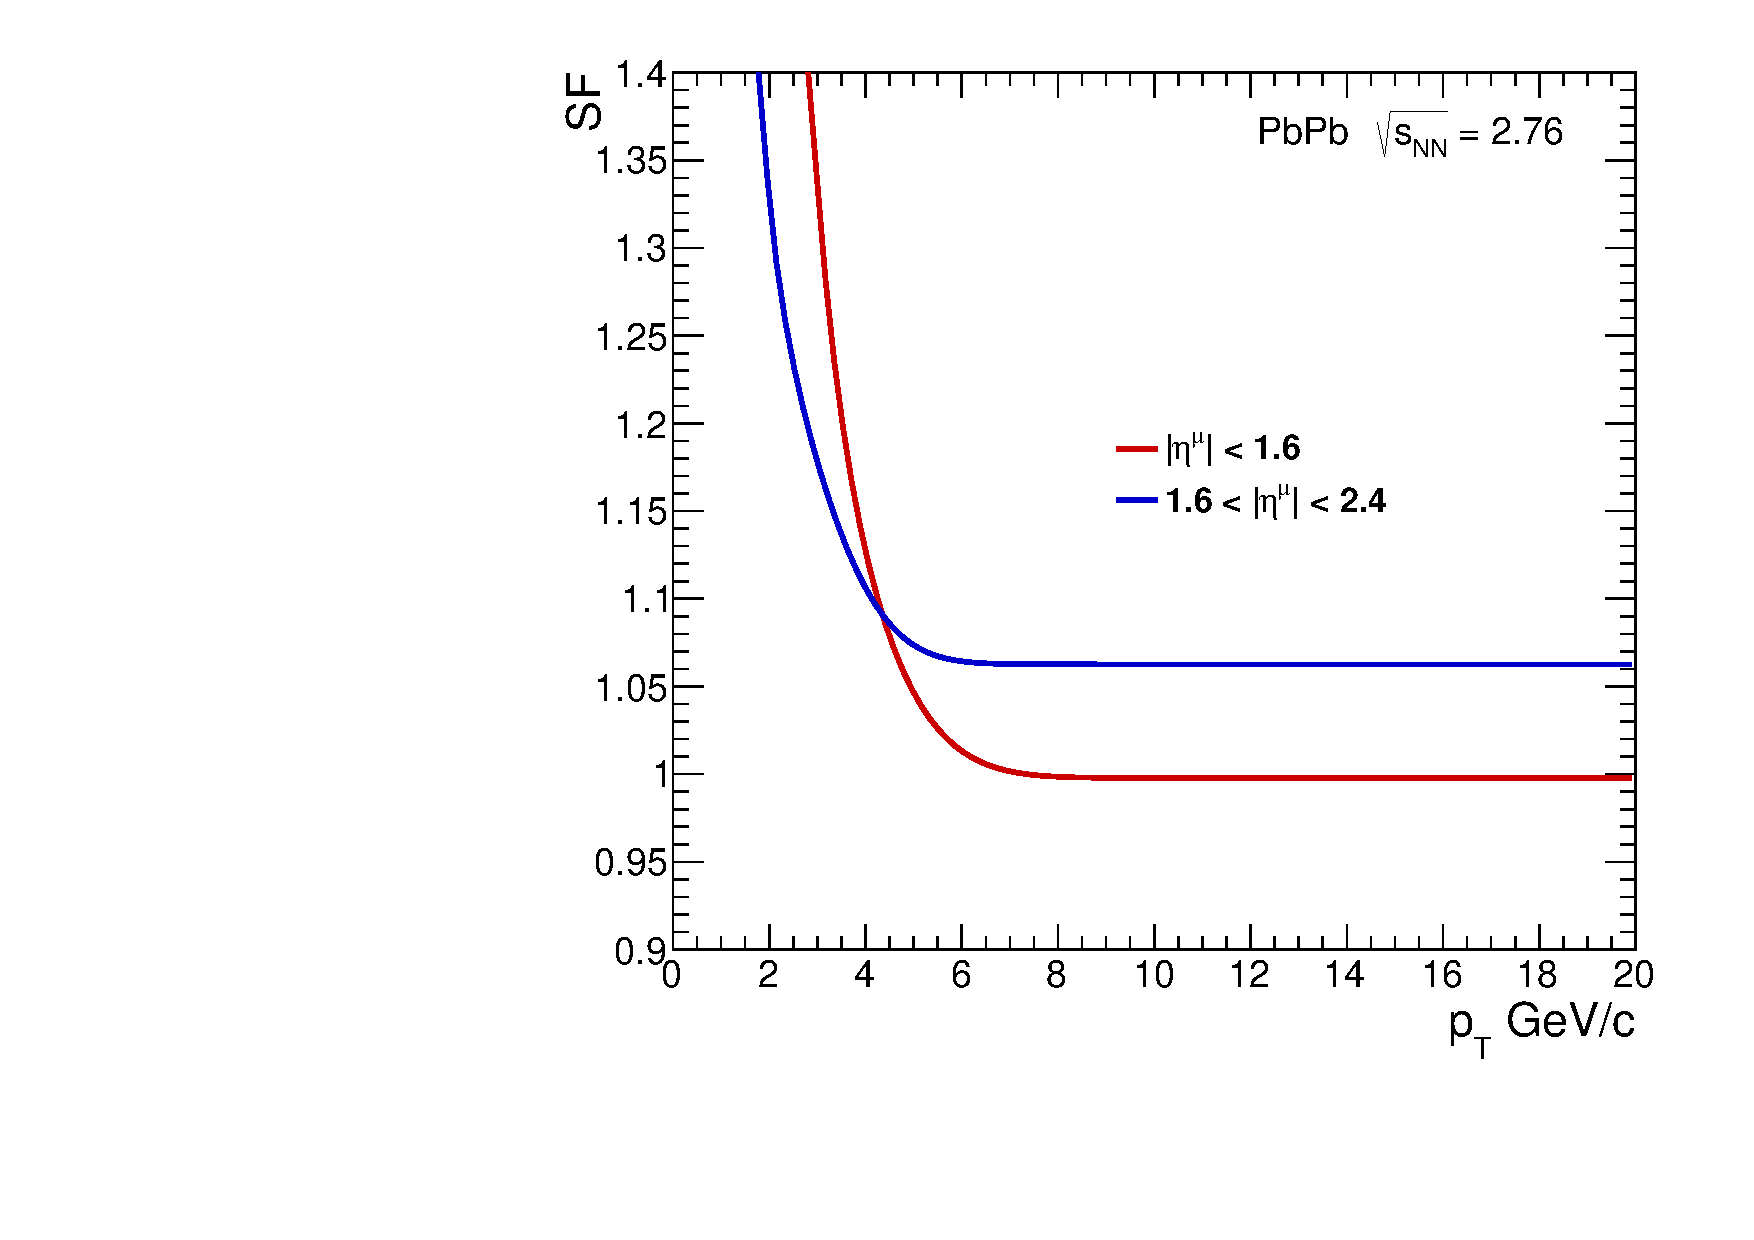
\includegraphics[width=0.4\textwidth]{Chapters/aCorrection/scale_factor_pbpb.pdf}
    \caption{
      Left: \Ctnp\ correction functions \vs. probe muon \pt, in $pp$ collisions.
      Right: \Ctnp\ correction functions \vs. probe muon \pt, in PbPb collisions.
    }
    \label{fig:SF}
  \end{center}
\end{figure}


To correct our dimuon efficiencies, each dimuon entry in the numerator of \eff\ in
Equation~\ref{eq:efficiency} is weighted by \Ctnp$_1\times$\Ctnp$_2$,
i.e. the product of \Ctnp\
computed at \pt-\Pgh\ of the first muon and \Ctnp\ computed at
\pt-\Pgh\ of the second muon. This has the effect of shifting the
dimuon efficiencies up, as can be seen in fig~\ref{fig:dimueff_SF}. It
can be noted that the efficiencies preserve the same trend after being
weighted with the \Ctnp\ corrections.

\begin{figure}
  \begin{center}
    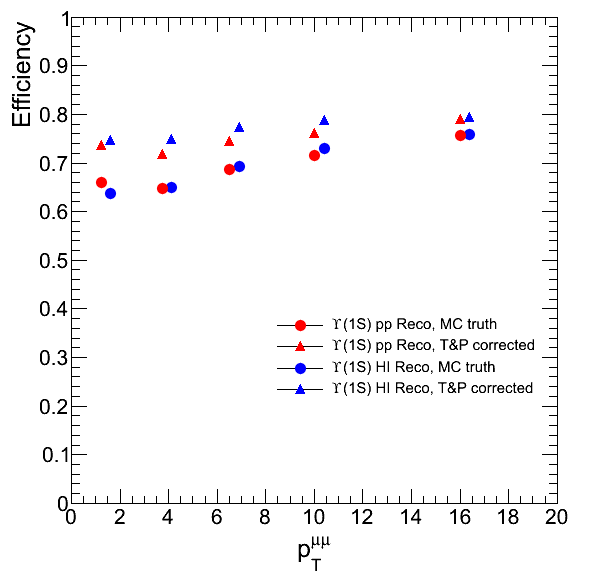
\includegraphics[width=0.49\textwidth]{Chapters/aCorrection/TnPCorrection_Pt.png}
    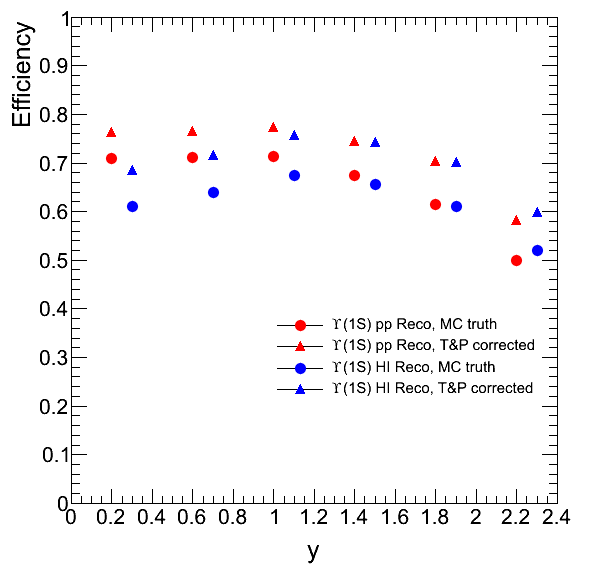
\includegraphics[width=0.49\textwidth]{Chapters/aCorrection/TnPCorrection_Rap.png}
    \caption{
      Dimuon efficiencies applied to $pp$ (red) and PbPb data
      (blue), in analysis bins of \pt (left) and \y\ (right). In both
      panels, triangles represent the efficiency correction obtained
      from simulation ('MC truth') and circles represent the
      same efficiency after applying the tag and probe corrective
      factors \Ctnp.
    }
    \label{fig:dimueff_SF}
  \end{center}
\end{figure}

% To illustrate the effect of the \Ctnp\ weighting on the dimuon
% efficiencies, the ratio \eff($\mu\mu$)$_{\rm {weighted}}$/\eff($\mu\mu$) before and after weighting is
% presented in Figure~\ref{sec:w_wo_tnp}, for pp and PbPb samples. One
% can see the effect of the weighting decrease as expected at higher
% \pt.

% \begin{figure}
%   \begin{center}
%     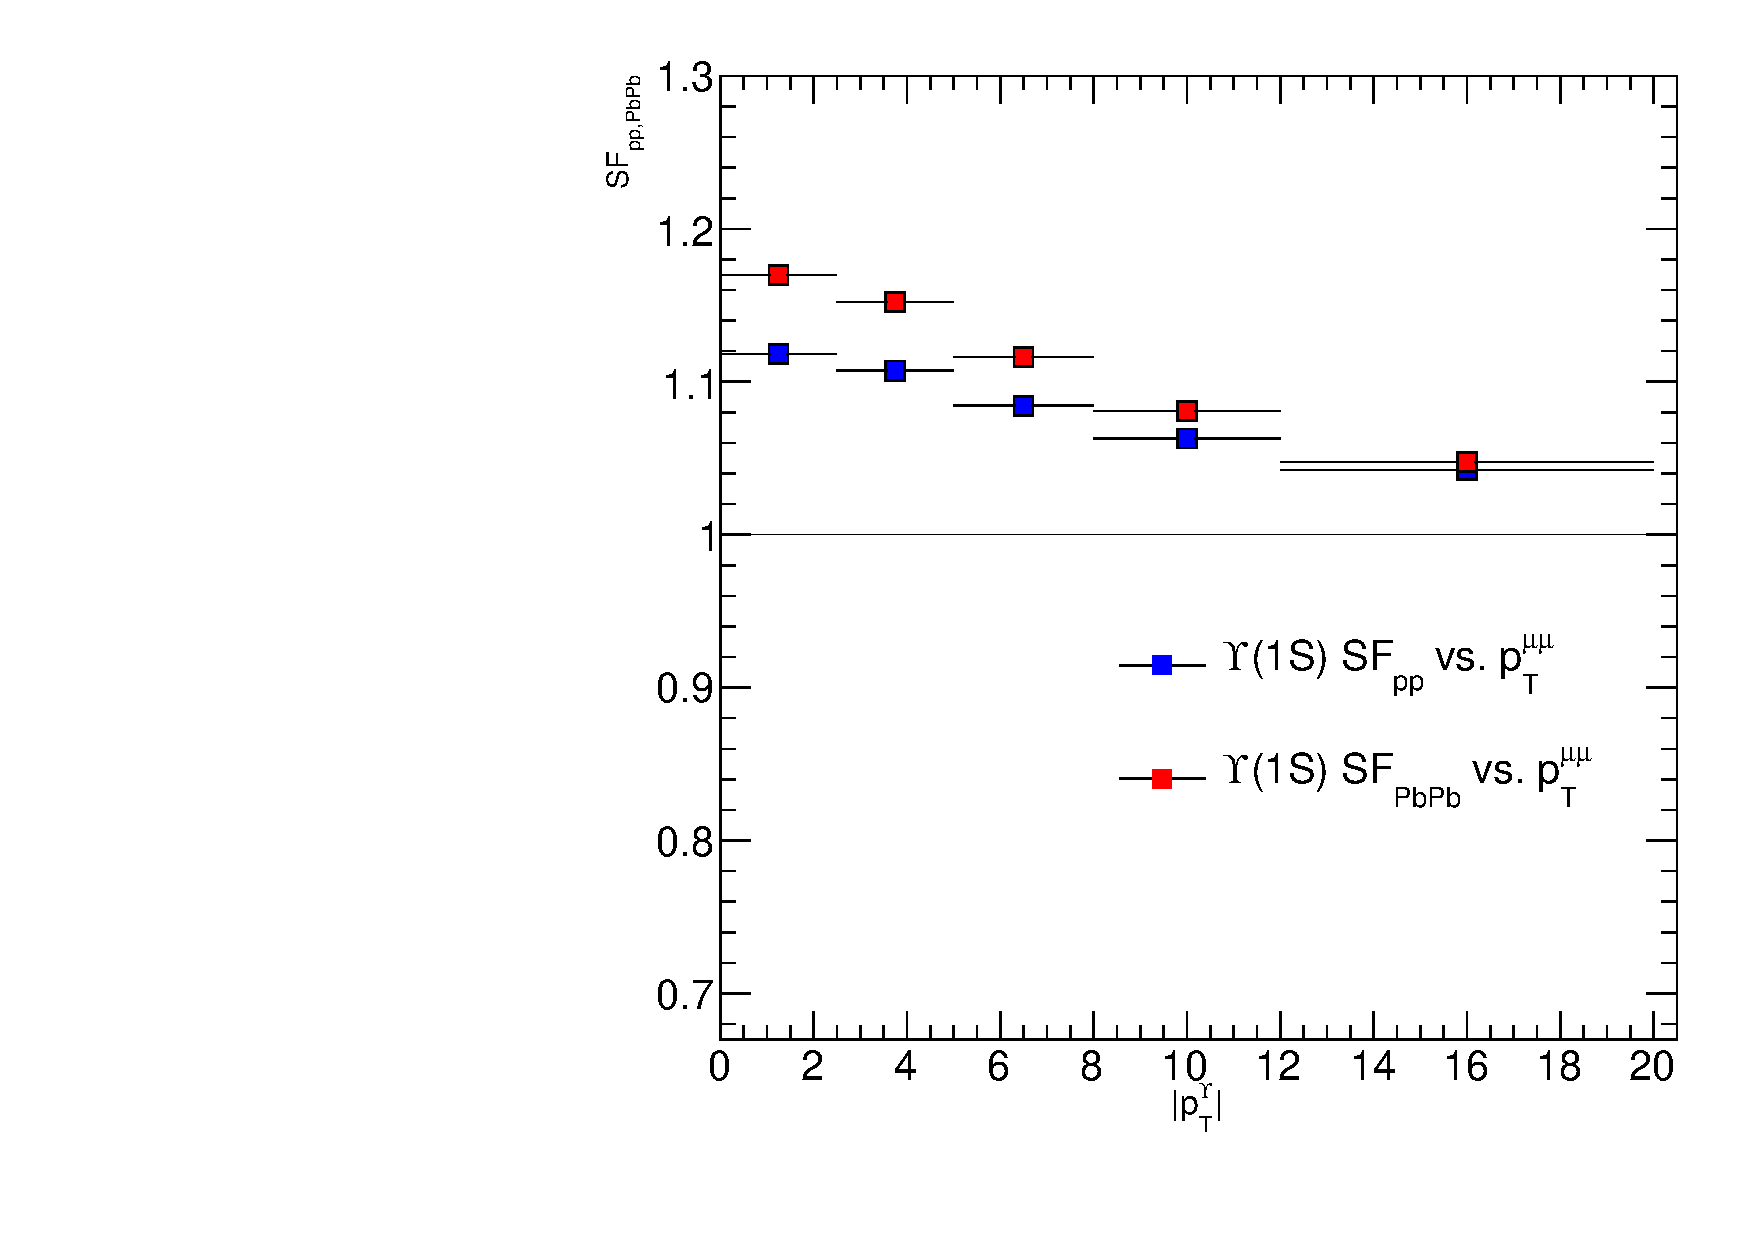
\includegraphics[width=0.6\textwidth]{Chapters/aCorrection/Tnp_SFcomp.pdf}
%     \caption{
%      Ratio \eff($\mu\mu$)$_{\rm {weighted}}$/\eff($\mu\mu$) as a
%      function of \pt.
%     }
%     \label{fig:w_wo_tnp}
%   \end{center}
% \end{figure}

% \begin{equation}
% \eff(\mu\mu)_{\rm weighted} = \frac{N^{\mu\mu}_{\RECO}}{N_{\acc}}
% \end{equation} 

% $\epsilon^{\mathrm{c}}_{\mu\mu} = \dfrac{N_{\mathrm{Reco}}\left(p^{\Upsilon}_{T},|y|^{\Upsilon},N_{coll};w(p^{\mu_{1}}_{T});w(p^{\mu_{2}}_{T})\right)}{N_{\mathrm{Acc}}}$, with $w(p^{\mu_{i}}_{T}) = \alpha\dfrac{\epsilon^{\mu^{i}}_{DATA}}{\epsilon^{\mu^{i}}_{MC}} $%= \alpha\dfrac{\dfrac{\left(x-\mu^{i}\right)}}{\sigma}}{...}$ % {\verbatim{TMath::Erf}(x-\mu^{i})_{DATA}}{\epsilon^{\mu^{i}}_{MC}}
% The significances $\sigma_{pp,AA}$ are computed for three regions of the detector. \\ Care has been taken
% $\sigma = \dfrac{S_{MC}}{\sqrt{S_{MC}+B_{L;R}}}$
\subsection{Systematic uncertainties}
\label{sec:tnp_syst}

Since the Tag and Probe method is based on simulations and data, the
reliability of the result is largely dependent on the statistics
available in data. In our case study, the PbPb collisions yield a
limited statistical precision on forward pseudorapidity muons. 

Another source of uncertainty comes from the Tag and Probe 
settings. Let me take a concrete example: in the efficiency of track
reconstruction, the tag (global muon with a good quality track) is
matched to a standalone muon (the probe). This probe passes the
selection if it is also a global muon, i.e. if it is matched to a good
quality track. In this case, it is difficult to assess the probability
that another track very close in pseudorapidity passed the matching to
the standalone in place of the actual muon track. This is especially
important in a high multiplicity environment such as heavy ion
collisions, and can yield a wrong, larger tracking efficiency. 

To evaluate a systematic accounting for this, the $\eff^{data}$
is recomputed for tag-probe pairs where the probe \pt\ requirement is
tighter (probe \pt > 5 \GeVc). To get an idea of the statistical uncertainty on the \Ctnp\ weighting procedure,
the $\eff^{data}_{\pt > 5}$ and $\eff^{data}_{\pt > 3.5}$ are taken as seeds for
100 random generations following asymmetric Gaussian
distributions, for each probe \pt setting. The varied efficiencies are refitted with an error
function, which leads to 200 variations on the \Ctnp. The resulting
variations on \Ctnp\ are presented for the pp efficiencies in
Figure~\ref{fig:tnpVar_pp}, and for the PbPb efficiencies in
Figure~\ref{fig:tnpVar_PbPb}.


\begin{figure}
  \begin{center}
    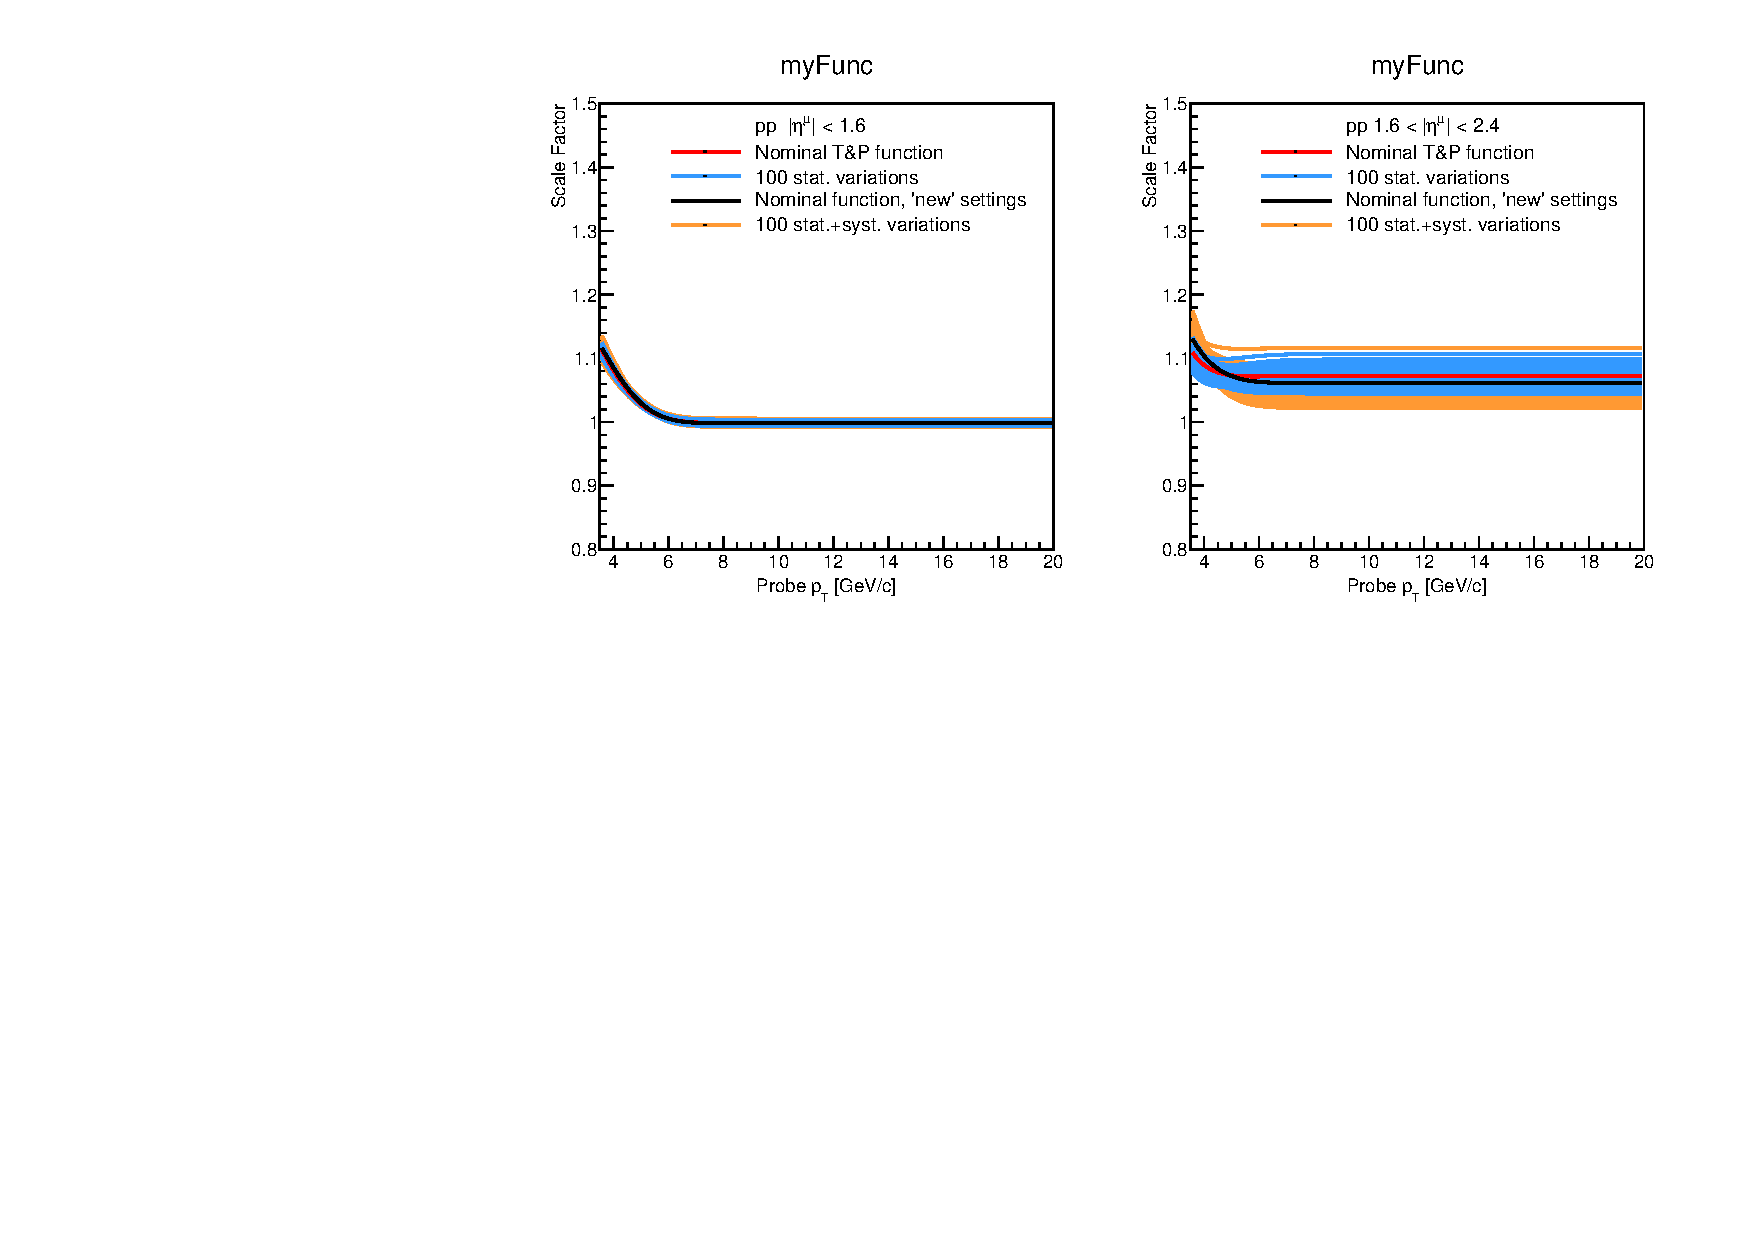
\includegraphics[width=0.9\textwidth]{Chapters/aCorrection/TNP_pp_100variations_new.pdf}
    \caption{
      100 variations of the $\eff^{data}$ part of \Ctnp ($pp$ collisions), using alternate
      tag-probe settings (orange) and using standard settings
      (blue). The blue curves make up for a statistical uncertainty of
      the procedure, while orange curves take also a systematic
      uncertainty into account.
    }
    \label{fig:tnpVar_pp}
  \end{center}
\end{figure}

 We can see that modifying the probe \pt\ requirements does not change
 the nominal \Ctnp\ function, as can be seen in red and black curves
 of Figures~\ref{fig:tnpVar_pp} and~\ref{fig:tnpVar_PbPb}. It was also checked
that the $\eff^{MC}$ part of \Ctnp\ remains unchanged after requesting
(probe \pt > 5 \GeVc). However, the blue curves, which are the 100
variations without changing the probe requirement, yield a reduced
uncertainty compared to the orange curves, which represent a
combination of the statistical and systematic uncertainty of the Tag
and Probe method. 

\begin{figure}
  \begin{center}
    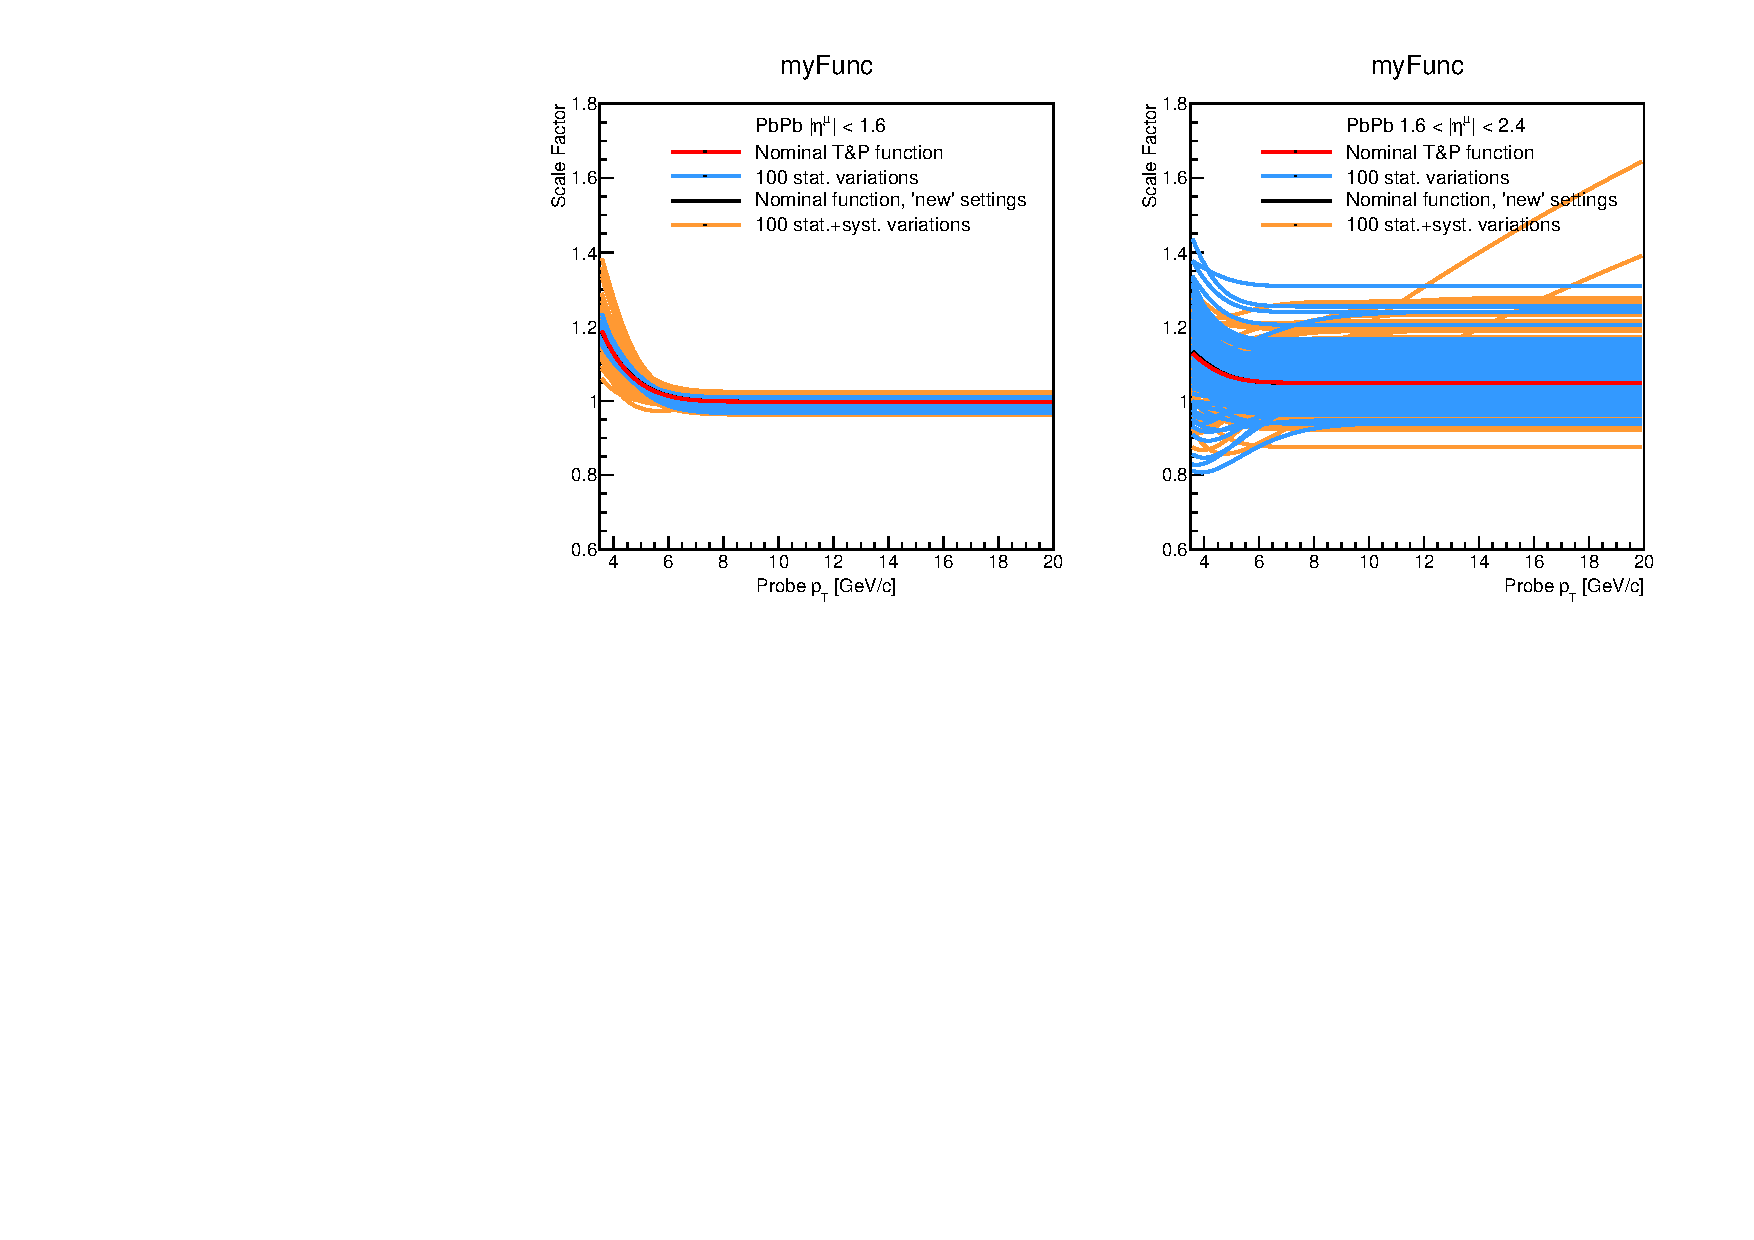
\includegraphics[width=0.9\textwidth]{Chapters/aCorrection/TNP_pbpb_100variations_newSettings_15-001.pdf}
    \caption{
      100 variations of the $\eff^{data}$ part of \Ctnp (PbPb collisions), using alternate
      tag-probe settings (orange) and using standard settings
      (blue). The blue curves make up for a statistical uncertainty of
      the procedure, while orange curves take also a systematic
      uncertainty into account.
    }
    \label{fig:tnpVar_PbPb}
  \end{center}
\end{figure}

We can also see that pp efficiencies, being defined with more
statistics than in the PbPb case, yield smaller uncertainties. In both
cases, the muons measured in the forward region of the detector need
larger corrections, as expected.



The resulting 100 \Ctnp\ variations are used to reweight the dimuon
efficiencies. In the end, the uncertainty related to this
procedure is taken, for each dimuon efficiency bin, as the RMS of the
distribution of the 100 reweighted efficiencies. 


For the preliminary result presented in this thesis, the uncertainties
regarding the tag and probe procedure have been taken relatively
conservative. At the time of finalising the document, additional
studies aiming at a better assessment of the systematic uncertainties
and the efficiencies are
underway. The largest part of the work to be completed regards the
systematic uncertainties in the tracking efficiency, and a closure
test related the procedure. These improvements are to be included in
the final publication.
\vspace{0.3cm}
\fbox{
  \parbox{0.9\textwidth}
  {\textsf{In this section, I have laid out the basics of the Tag and
      Probe method, a standard method to attribute data-driven values to the
      efficiencies, of wide-spread use to dilepton analyses, in CMS and
      other experiments. We have seen that there is a difference between our
      estimation of the efficiencies using the MC simulations and the
      data. This contributes to the \acc\eff\ factor. The following section
      will sum up the findings on \acc\eff\ and weightings applied, to
      extract the net correction applied to the raw yields.}}
}



\section{Summary}
\subsection{Summary of \texorpdfstring{\PgU(nS)}{Y(nS)} corrections}
\label{sec:aCorr_summary}
In the previous section, the following corrections and systematic
uncertainties were presented:
\begin{itemize}
\item For each \PgU\ state in $pp$ and PbPb data:
  \begin{itemize}
  \item[-] \acc\eff(\Pgm\Pgm), the dimuon acceptance and efficiency,
    differential in \pt, \y (or \Npart) of the \PgU\ state,
  \item[-] \Ctnp$_1\times$\Ctnp$_2$, acting as an event-by-event
    weight to candidates entering in the
    numerator of \acc\eff, changing \acc\eff(\Pgm\Pgm) in
    \acc\eff(\Pgm\Pgm)$_{w}$,
  \item[-] systematic uncertainties on assumed spectra (and centrality
    determination in PbPb), computed for each \pt, \y (\Npart) bin of
    \acc\eff,
  \item[-] systematic and statistical uncertainties on the
    Tag and Probe method, acting directly as an uncertainty on the
    \acc\eff(\Pgm\Pgm)$_{w}$ correction.
  \end{itemize}
This is summarised in Figure~\ref{fig:aet_final}.
\item Common to all states, the tracking efficiency, taken as a global
  systematic uncertainty:
  \begin{itemize}
  \item[-] 1.7\% for each muon track in pp,
  \item[-] 5\% for each muon track in PbPb.
  \end{itemize}
  This will appear as a global uncertainty band in \RAA, in Section~\ref{subsec:raa}.
\end{itemize}

\label{sec:aet_summary}
Figure~\ref{fig:aet_final} shows the total \acc\eff$_{\rm weighted}$
dimuon correction for all \PgU\ states, \vs. the dimuon rapidity. Both
 plots show that \PgUa\ is reconstructed more
efficiently than \PgUb: this is due to the kinematic cuts applied to
the \PgUa, increasing the acceptance fraction for the \PgUa.%  On
% the left hand side we can see however that the \PgUc\ is still more
% efficiently reconstructed than the ground state. This is attributed to
% the higher mass of \PgUc, 10.355 GeV/$c^{2}$, which in turn makes the
% acceptance and efficiency larger for this particles than for the
% others. 

\begin{figure}
  \begin{center}
    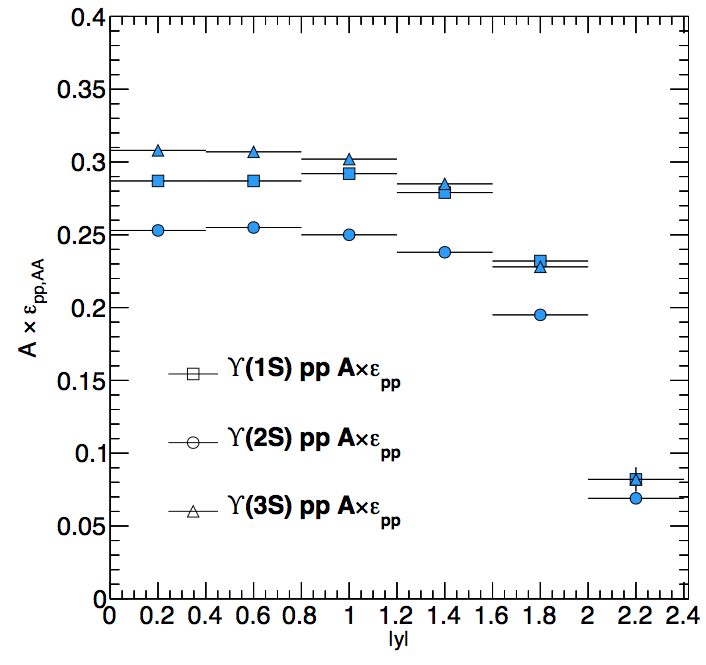
\includegraphics[width=0.45\textwidth]{Chapters/aCorrection/pp_aet.png}
    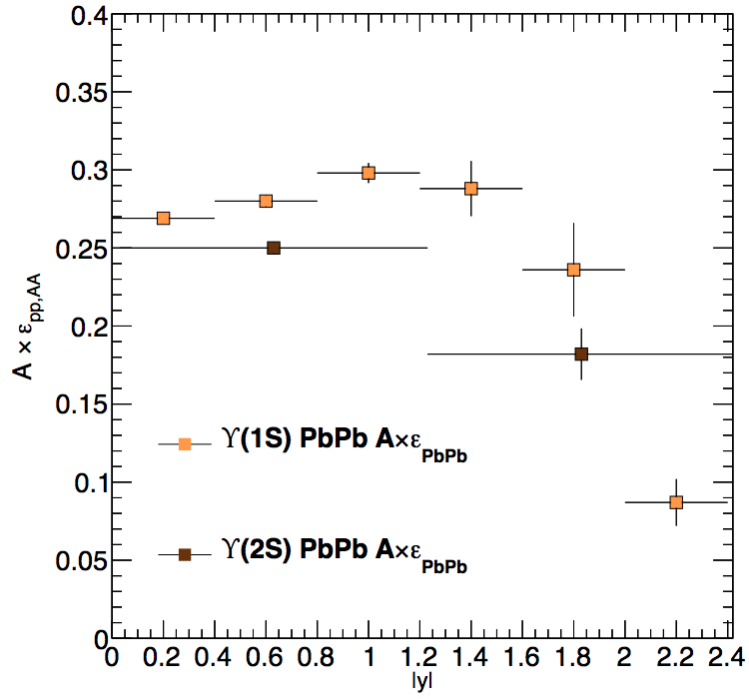
\includegraphics[width=0.45\textwidth]{Chapters/aCorrection/AA_aet.png}
    \caption{
      Total correction factor \acc\eff$_{w}$ applied to
      \PgU\ states, with uncertainties. 
      Left: correction for pp yields. Right: correction for PbPb yields.
    }
    \label{fig:aet_final}
  \end{center}
\end{figure}

One can also note the increasing uncertainty at large rapidities. This
is due to both Tag and Probe and the shape uncertainties, having more
effect in PbPb at high rapidities as shown in
Table~\ref{totalacceff_pbpb}. 
\subsection{Tabulated results}
The tabulated version of \acc\eff$_{w}$ corrections is presented in
Table~\ref{finalacceff_pp} for \PgU\ states in $pp$ collisions, and in
Table~\ref{finalacceff_pbpb} for \PgU\ states in PbPb collisions. Since the statistical
uncertainty in \acc\ and \eff\ is very small and only due to the size of
our simulations (not dependent of the measurement, but on the number
of generated events), I add it in quadrature all the sources of
systematic uncertainties, at the exception of the tracking
uncertainties which are global and do not appear here. As a
consequence, the results are shown in the format \acc\eff$_w$~$\pm~\sigma$, where $\sigma$ is the quadratic sum of all statistical and
systematic uncertainties covered in Sections~\ref{sec:acceff_syst} and
\ref{sec:tnp_syst}. 



\begin{table}
\begin{center}
\begin{tabular}{|c|c|c|c|}
\hline
\pt [\GeVc]& \acc\eff$_w$[1S](\pt)      & |\y|     &      \acc\eff$_w$[1S](\y) \\

\hline                                       
0-2.5             &0.339 $\pm$ 0.008   & 0-0.4   &0.300 $\pm$ 0.003 \\
2.5-5             &0.214 $\pm$ 0.004   & 0.4-0.8 &0.299 $\pm$ 0.003 \\
5-8               &0.207 $\pm$ 0.006   & 0.8-1.2 &0.303 $\pm$ 0.002 \\
8-12              &0.284 $\pm$ 0.008   & 1.2-1.6 &0.289 $\pm$ 0.003 \\
12-20             &0.404 $\pm$ 0.011   & 1.6-2   &0.238 $\pm$ 0.003 \\
\cline{1-2}
\textbf{0-100}    &\textbf{0.262 $\pm$ 0.002}  & 2-2.4   & 0.085 $\pm$ 0.002 \\             
\hline                           
\end{tabular}
\begin{tabular}{|c|c|c|c|}
\hline
\pt [\GeVc]& \acc\eff$_w$[2S](\pt)      & |\y|     &      \acc\eff$_w$[2S](\y) \\

\hline                                       
0-2.5             &0.293 $\pm$ 0.007  & 0-0.4   &0.253 $\pm$ 0.004\\
2.5-5             &0.171 $\pm$ 0.004  & 0.4-0.8 &0.255 $\pm$ 0.004\\
5-8               &0.172 $\pm$ 0.005  & 0.8-1.2 &0.250 $\pm$ 0.003\\
8-12              &0.246 $\pm$ 0.008  & 1.2-1.6 &0.238 $\pm$ 0.004\\
12-20             &0.379 $\pm$ 0.011  & 1.6-2   &0.195 $\pm$ 0.003\\
\cline{1-2}
\textbf{0-100}    &\textbf{0.218 $\pm$ 0.001}  & 2-2.4   &0.069 $\pm$ 0.002\\             
\hline                           
\end{tabular}
\begin{tabular}{|c|c|c|c|}
\hline
\pt [\GeVc]& \acc\eff$_w$[3S](\pt)      & |\y|     &      \acc\eff$_w$[3S](\y) \\
\hline                                       
0-2.5             &0.361 $\pm$ 0.009 & 0-0.4   &0.308 $\pm$ 0.003\\
2.5-5             &0.214 $\pm$ 0.005 & 0.4-0.8 &0.307 $\pm$ 0.003\\
5-8               &0.199 $\pm$ 0.005 & 0.8-1.2 &0.302 $\pm$ 0.003\\
8-12              &0.267 $\pm$ 0.008 & 1.2-1.6 &0.285 $\pm$ 0.003\\
12-20             &0.389 $\pm$ 0.011 & 1.6-2   &0.228 $\pm$ 0.003\\
\cline{1-2}
\textbf{0-100}    &\textbf{0.263 $\pm$ 0.001} & 2-2.4   &0.082 $\pm$ 0.002\\             
\hline                           
\end{tabular}
\caption{Final \acc\eff$_w$ for all \PgU\ states in the pp
  case. All uncertainties have been summed in quadrature, except
  tracking (not shown here). Integrated results displayed
  in bold font.}
\label{finalacceff_pp}
\end{center}
\end{table}
%%%%%%% table for pbpb
\begin{table}[t]
\begin{center}
\begin{tabular}{|c|c|c|c|}
\hline
\pt [\GeVc]& \acc\eff$_w$[1S](\pt)      & |\y|     &      \acc\eff$_w$[1S](\y) \\
\hline                                       
0-2.5             &0.315 $\pm$ 0.022 & 0-0.4   & 0.269 $\pm$ 0.012 \\
2.5-5             &0.202 $\pm$ 0.013 & 0.4-0.8 & 0.280 $\pm$ 0.012 \\
5-8               &0.202 $\pm$ 0.012 & 0.8-1.2 & 0.298 $\pm$ 0.014 \\
8-12              &0.288 $\pm$ 0.016 & 1.2-1.6 & 0.289 $\pm$ 0.019 \\
12-20             &0.406 $\pm$ 0.020 & 1.6-2   & 0.237 $\pm$ 0.024 \\
\cline{1-2}
\textbf{0-100}    &\textbf{0.252 $\pm$ 0.014} & 2-2.4   & 0.087 $\pm$ 0.011 \\             
\hline \hline             
\end{tabular}
\begin{tabular}{|c|c|}
\hline
Centrality & \acc\eff$_w$[1S](Cent.)$_{\rm PbPb}$ \\
\hline
0\%-5\%   & 0.241 $\pm$ 0.010 \\
5\%-10\%  & 0.249 $\pm$ 0.012 \\
10\%-20\% & 0.253 $\pm$ 0.011 \\
20\%-30\% & 0.257 $\pm$ 0.011 \\
30\%-40\% & 0.258 $\pm$ 0.011 \\
40\%-50\% & 0.259 $\pm$ 0.011 \\
50\%-70\% & 0.262 $\pm$ 0.011 \\
70\%-100\%& 0.261 $\pm$ 0.011 \\
\hline                        
\end{tabular}
\begin{tabular}{|c|c|c|c|}
\hline
\pt [\GeVc]& \acc\eff$_w$[2S](\pt)      & |\y|     &      \acc\eff$_w$[2S](\y) \\
\hline                                       
0-5               &0.203 $\pm$ 0.009 & 0-1.2   & 0.250 $\pm$ 0.005 \\
5-12              &0.202 $\pm$ 0.010 & 1.2-2.4 & 0.182 $\pm$ 0.016 \\
12-20             &0.402 $\pm$ 0.021 & -  & - \\
\cline{1-2}
\textbf{0-100}             &\textbf{0.221 $\pm$ 0.009} & -  & - \\             
\hline        

\end{tabular}
\begin{tabular}{|c|c|}
\hline
Centrality & \acc\eff$_w$[2S](Cent.)$_{\rm PbPb}$ \\
\hline
0\%-10\%  & 0.213 $\pm$ 0.010\\
10\%-30\% & 0.220 $\pm$ 0.010\\
30\%-50\% & 0.224 $\pm$ 0.010\\
50\%-100\%& 0.226 $\pm$ 0.010\\

\hline                           
\end{tabular}
\caption{Final \acc\eff$_w$ for \PgUa,\PgUb\ states in the PbPb
  case. All uncertainties have been summed in quadrature, except
  tracking (not shown here). Integrated results displayed
  in bold font.}
\label{finalacceff_pbpb}
\end{center}
\end{table}



